% Options for packages loaded elsewhere
% Options for packages loaded elsewhere
\PassOptionsToPackage{unicode}{hyperref}
\PassOptionsToPackage{hyphens}{url}
\PassOptionsToPackage{dvipsnames,svgnames,x11names}{xcolor}
%
\documentclass[
  11pt,
  letterpaper,
  DIV=11,
  numbers=noendperiod]{scrartcl}
\usepackage{xcolor}
\usepackage[margin=2.5cm]{geometry}
\usepackage{amsmath,amssymb}
\setcounter{secnumdepth}{5}
\usepackage{iftex}
\ifPDFTeX
  \usepackage[T1]{fontenc}
  \usepackage[utf8]{inputenc}
  \usepackage{textcomp} % provide euro and other symbols
\else % if luatex or xetex
  \usepackage{unicode-math} % this also loads fontspec
  \defaultfontfeatures{Scale=MatchLowercase}
  \defaultfontfeatures[\rmfamily]{Ligatures=TeX,Scale=1}
\fi
\usepackage{lmodern}
\ifPDFTeX\else
  % xetex/luatex font selection
  \setmainfont[]{Times New Roman}
\fi
% Use upquote if available, for straight quotes in verbatim environments
\IfFileExists{upquote.sty}{\usepackage{upquote}}{}
\IfFileExists{microtype.sty}{% use microtype if available
  \usepackage[]{microtype}
  \UseMicrotypeSet[protrusion]{basicmath} % disable protrusion for tt fonts
}{}
\usepackage{setspace}
\makeatletter
\@ifundefined{KOMAClassName}{% if non-KOMA class
  \IfFileExists{parskip.sty}{%
    \usepackage{parskip}
  }{% else
    \setlength{\parindent}{0pt}
    \setlength{\parskip}{6pt plus 2pt minus 1pt}}
}{% if KOMA class
  \KOMAoptions{parskip=half}}
\makeatother
% Make \paragraph and \subparagraph free-standing
\makeatletter
\ifx\paragraph\undefined\else
  \let\oldparagraph\paragraph
  \renewcommand{\paragraph}{
    \@ifstar
      \xxxParagraphStar
      \xxxParagraphNoStar
  }
  \newcommand{\xxxParagraphStar}[1]{\oldparagraph*{#1}\mbox{}}
  \newcommand{\xxxParagraphNoStar}[1]{\oldparagraph{#1}\mbox{}}
\fi
\ifx\subparagraph\undefined\else
  \let\oldsubparagraph\subparagraph
  \renewcommand{\subparagraph}{
    \@ifstar
      \xxxSubParagraphStar
      \xxxSubParagraphNoStar
  }
  \newcommand{\xxxSubParagraphStar}[1]{\oldsubparagraph*{#1}\mbox{}}
  \newcommand{\xxxSubParagraphNoStar}[1]{\oldsubparagraph{#1}\mbox{}}
\fi
\makeatother


\usepackage{longtable,booktabs,array}
\usepackage{calc} % for calculating minipage widths
% Correct order of tables after \paragraph or \subparagraph
\usepackage{etoolbox}
\makeatletter
\patchcmd\longtable{\par}{\if@noskipsec\mbox{}\fi\par}{}{}
\makeatother
% Allow footnotes in longtable head/foot
\IfFileExists{footnotehyper.sty}{\usepackage{footnotehyper}}{\usepackage{footnote}}
\makesavenoteenv{longtable}
\usepackage{graphicx}
\makeatletter
\newsavebox\pandoc@box
\newcommand*\pandocbounded[1]{% scales image to fit in text height/width
  \sbox\pandoc@box{#1}%
  \Gscale@div\@tempa{\textheight}{\dimexpr\ht\pandoc@box+\dp\pandoc@box\relax}%
  \Gscale@div\@tempb{\linewidth}{\wd\pandoc@box}%
  \ifdim\@tempb\p@<\@tempa\p@\let\@tempa\@tempb\fi% select the smaller of both
  \ifdim\@tempa\p@<\p@\scalebox{\@tempa}{\usebox\pandoc@box}%
  \else\usebox{\pandoc@box}%
  \fi%
}
% Set default figure placement to htbp
\def\fps@figure{htbp}
\makeatother





\setlength{\emergencystretch}{3em} % prevent overfull lines

\providecommand{\tightlist}{%
  \setlength{\itemsep}{0pt}\setlength{\parskip}{0pt}}



 


\usepackage{booktabs}
\usepackage{longtable}
\usepackage{array}
\usepackage{multirow}
\usepackage{wrapfig}
\usepackage{float}
\usepackage{colortbl}
\usepackage{pdflscape}
\usepackage{tabularx}
\usepackage{xltabular}
\usepackage{threeparttable}
\usepackage{threeparttablex}
\usepackage[normalem]{ulem}
\usepackage{makecell}
\usepackage{xcolor}
\usepackage{xcolor}
\newcommand{\ins}[1]{\textcolor{red}{[#1]}}
\newcommand{\conf}[1]{\textcolor{red}{[CONFIRM: #1]}}
\usepackage{booktabs}
\usepackage{longtable}
\usepackage{array}
\KOMAoption{captions}{tableheading}
\makeatletter
\@ifpackageloaded{caption}{}{\usepackage{caption}}
\AtBeginDocument{%
\ifdefined\contentsname
  \renewcommand*\contentsname{Table of contents}
\else
  \newcommand\contentsname{Table of contents}
\fi
\ifdefined\listfigurename
  \renewcommand*\listfigurename{List of Figures}
\else
  \newcommand\listfigurename{List of Figures}
\fi
\ifdefined\listtablename
  \renewcommand*\listtablename{List of Tables}
\else
  \newcommand\listtablename{List of Tables}
\fi
\ifdefined\figurename
  \renewcommand*\figurename{Figure}
\else
  \newcommand\figurename{Figure}
\fi
\ifdefined\tablename
  \renewcommand*\tablename{Table}
\else
  \newcommand\tablename{Table}
\fi
}
\@ifpackageloaded{float}{}{\usepackage{float}}
\floatstyle{ruled}
\@ifundefined{c@chapter}{\newfloat{codelisting}{h}{lop}}{\newfloat{codelisting}{h}{lop}[chapter]}
\floatname{codelisting}{Listing}
\newcommand*\listoflistings{\listof{codelisting}{List of Listings}}
\makeatother
\makeatletter
\makeatother
\makeatletter
\@ifpackageloaded{caption}{}{\usepackage{caption}}
\@ifpackageloaded{subcaption}{}{\usepackage{subcaption}}
\makeatother
\usepackage{bookmark}
\IfFileExists{xurl.sty}{\usepackage{xurl}}{} % add URL line breaks if available
\urlstyle{same}
\hypersetup{
  colorlinks=true,
  linkcolor={blue},
  filecolor={Maroon},
  citecolor={Blue},
  urlcolor={Blue},
  pdfcreator={LaTeX via pandoc}}


\title{\ins{TITLE}}
\author{\ins{Authors and affiliations}}
\date{2026-11-20}
\begin{document}
\maketitle


\setstretch{1.5}
\section*{Abstract}\label{abstract}
\addcontentsline{toc}{section}{Abstract}

Toothed whales are the most diverse group of top predators in the
Southern Ocean, yet where and when they occur in Antarctic waters,
particularly in winter, remains poorly known. Many of these species
forage hundreds of metres below the surface, where Antarctic Circumpolar
Current, Bellingshausen Sea and Weddell Sea waters meet around the
Antarctic Peninsula. Habitat studies, however, have relied mostly on
surface conditions and on summer ship-based surveys. How odontocete
occurrence relates to sea ice and to conditions at foraging depth has
therefore not been tested. Here we show, using year-round passive
acoustic recordings at three sites in the South Shetland Islands
(2014--2016), that sea ice and anomalous ocean conditions at the surface
and at depth structure odontocete occurrence. Sperm Whales and Killer
Whales were detected under more than 50\% sea-ice cover, whereas
long-finned pilot whales were never detected above 34\% cover and two
beaked whale signal types (BW29 and BW37) never above 13\%. After the
seasonal cycle was removed, warmer-than-usual surface water was
associated with pilot whale presence at all three sites. Beaked whale
and sperm whale presence was linked to surface fronts, and to mid-water
eddy activity and deep-layer temperature anomalies, depending on site.
Responses differed among sites that sample distinct water masses,
indicating that habitat associations are local rather than species-wide.
As sea ice retreats and warm Circumpolar Deep Water increasingly reaches
the Antarctic Peninsula shelf, subsurface conditions may shape
odontocete distribution as much as surface conditions do. Ocean
reanalyses validated against in-situ profiles offer a way to include
them in habitat models.
\conf{wording of the habitat sentences after the final run}

\section{Introduction}\label{introduction}

\ins{Introduction to be written}

\section{Methods}\label{methods}

\subsection{Study area}\label{sec-study}

Passive acoustic data were collected at three sites along the northern
shelf slope of the South Shetland Islands, Antarctica: Elephant Island
(EI; 60°53.214′S, 55°57.238′W; 762 m depth), King George Island (KGI;
61°27.469′S, 57°56.515′W; 768 m), and Clarence Island (CI; 61°15.112′S,
53°29.006′W; 1033 m) (Figure~\ref{fig-map}).

The South Shetland Islands lie at the confluence of water masses from
the Drake Passage, the Bellingshausen Sea, and the Weddell Sea
(Figure~\ref{fig-map}). To the north, the Southern Antarctic Circumpolar
Current Front and the Southern Boundary of the Antarctic Circumpolar
Current (ACC) follow the continental slope (Orsi et al.~1995), and the
Southern Boundary passes close to the EI and KGI sites. Upper
Circumpolar Deep Water from the ACC intrudes onto the northern South
Shetland shelf as modified Circumpolar Deep Water (mCDW), particularly
west of the Shackleton Transverse Ridge, whereas shelf waters are
exported offshore north of Elephant Island, just downstream of the EI
site (Zhou et al.~2013, Damini et al.~2025). South of the islands, the
Bransfield Current flows northeastward along the southern slope of the
South Shetland Islands, carrying relatively warm and fresh Transitional
Zonal Water with Bellingshausen Sea influence (TBW; Sangrà et al.~2011,
2017, Veny et al.~2022), with part of the flow recirculating
southwestward along the northern side of the islands (Dotto et al.~2021,
Damini et al.~2025). Colder and saltier Transitional Zonal Water with
Weddell Sea influence (TWW) enters Bransfield Strait from the east via
the Antarctic Coastal Current and the Antarctic Slope Front around the
tip of the Antarctic Peninsula (Heywood et al.~2004, Thompson et
al.~2009) and is separated from TBW by the Peninsula Front (Sangrà et
al.~2011, Veny et al.~2024). East of Elephant Island, the Antarctic
Slope Front bifurcates over the South Scotia Ridge near the CI site,
forming a westward branch and a quasi-stationary eddy (Thompson et
al.~2009). The three sites therefore sample contrasting oceanographic
regimes: EI near the shelf-water export pathway at the Shackleton Gap,
KGI on the northern South Shetland slope beneath the Southern Boundary
of the ACC, and CI under stronger Weddell Sea influence
\conf{characterization of each site}.

High-frequency Acoustic Recording Packages (HARPs; Wiggins \& Hildebrand
2007) were deployed sequentially at the three sites, sampling at 200
kHz. Recordings spanned 5 March -- 17 July 2014 at EI (134.5 days), 10
February 2015 -- 29 January 2016 at KGI (353.6 days), and 3 February --
2 December 2016 at CI (302.2 days) (Table \ref{tab:deploy}). The EI and
KGI recorders were duty-cycled (5 min on every 6 min and 10 min on every
13.33 min, respectively), whereas the CI recorder recorded continuously.

Bathymetry for the study-area map (Figure~\ref{fig-map}) was obtained
from the Global Multi-Resolution Topography synthesis (GMRT v4.4.1; Ryan
et al.~2009; accessed 11 May 2026 via GMRT MapTool) and contoured at
500-m intervals. Regional circulation (Figure~\ref{fig-map}) was
illustrated with long-term (2009--2021) mean surface currents from the
Copernicus Marine Service global ocean physics reanalysis
(GLOBAL\_MULTIYEAR\_PHY\_001\_030, dataset version 202311, monthly means
at 0.5 m; accessed 17 November 2026) and the positions of the Southern
Antarctic Circumpolar Current Front and the Southern Boundary of the
Antarctic Circumpolar Current from Orsi et al.~(1995).

\begin{table}[!h]
\centering
\caption{\label{tab:deploy}HARP deployments.}
\centering
\fontsize{9}{11}\selectfont
\begin{tabular}[t]{lllrllrl}
\toprule
Site & Latitude & Longitude & Depth (m) & Start (UTC) & End (UTC) & Duration (d) & Duty cycle\\
\midrule
EI & 60°53.214′S & 55°57.238′W & 762 & 2014-03-05 00:00 & 2014-07-17 12:03 & 134.5 & 5 of 6 min\\
KGI & 61°27.469′S & 57°56.515′W & 768 & 2015-02-10 00:00 & 2016-01-29 13:15 & 353.6 & 10 of 13.33 min\\
CI & 61°15.112′S & 53°29.006′W & 1033 & 2016-02-03 23:59 & 2016-12-02 05:15 & 302.2 & Continuous\\
\bottomrule
\end{tabular}
\end{table}

\begin{figure}[htbp]

\centering{

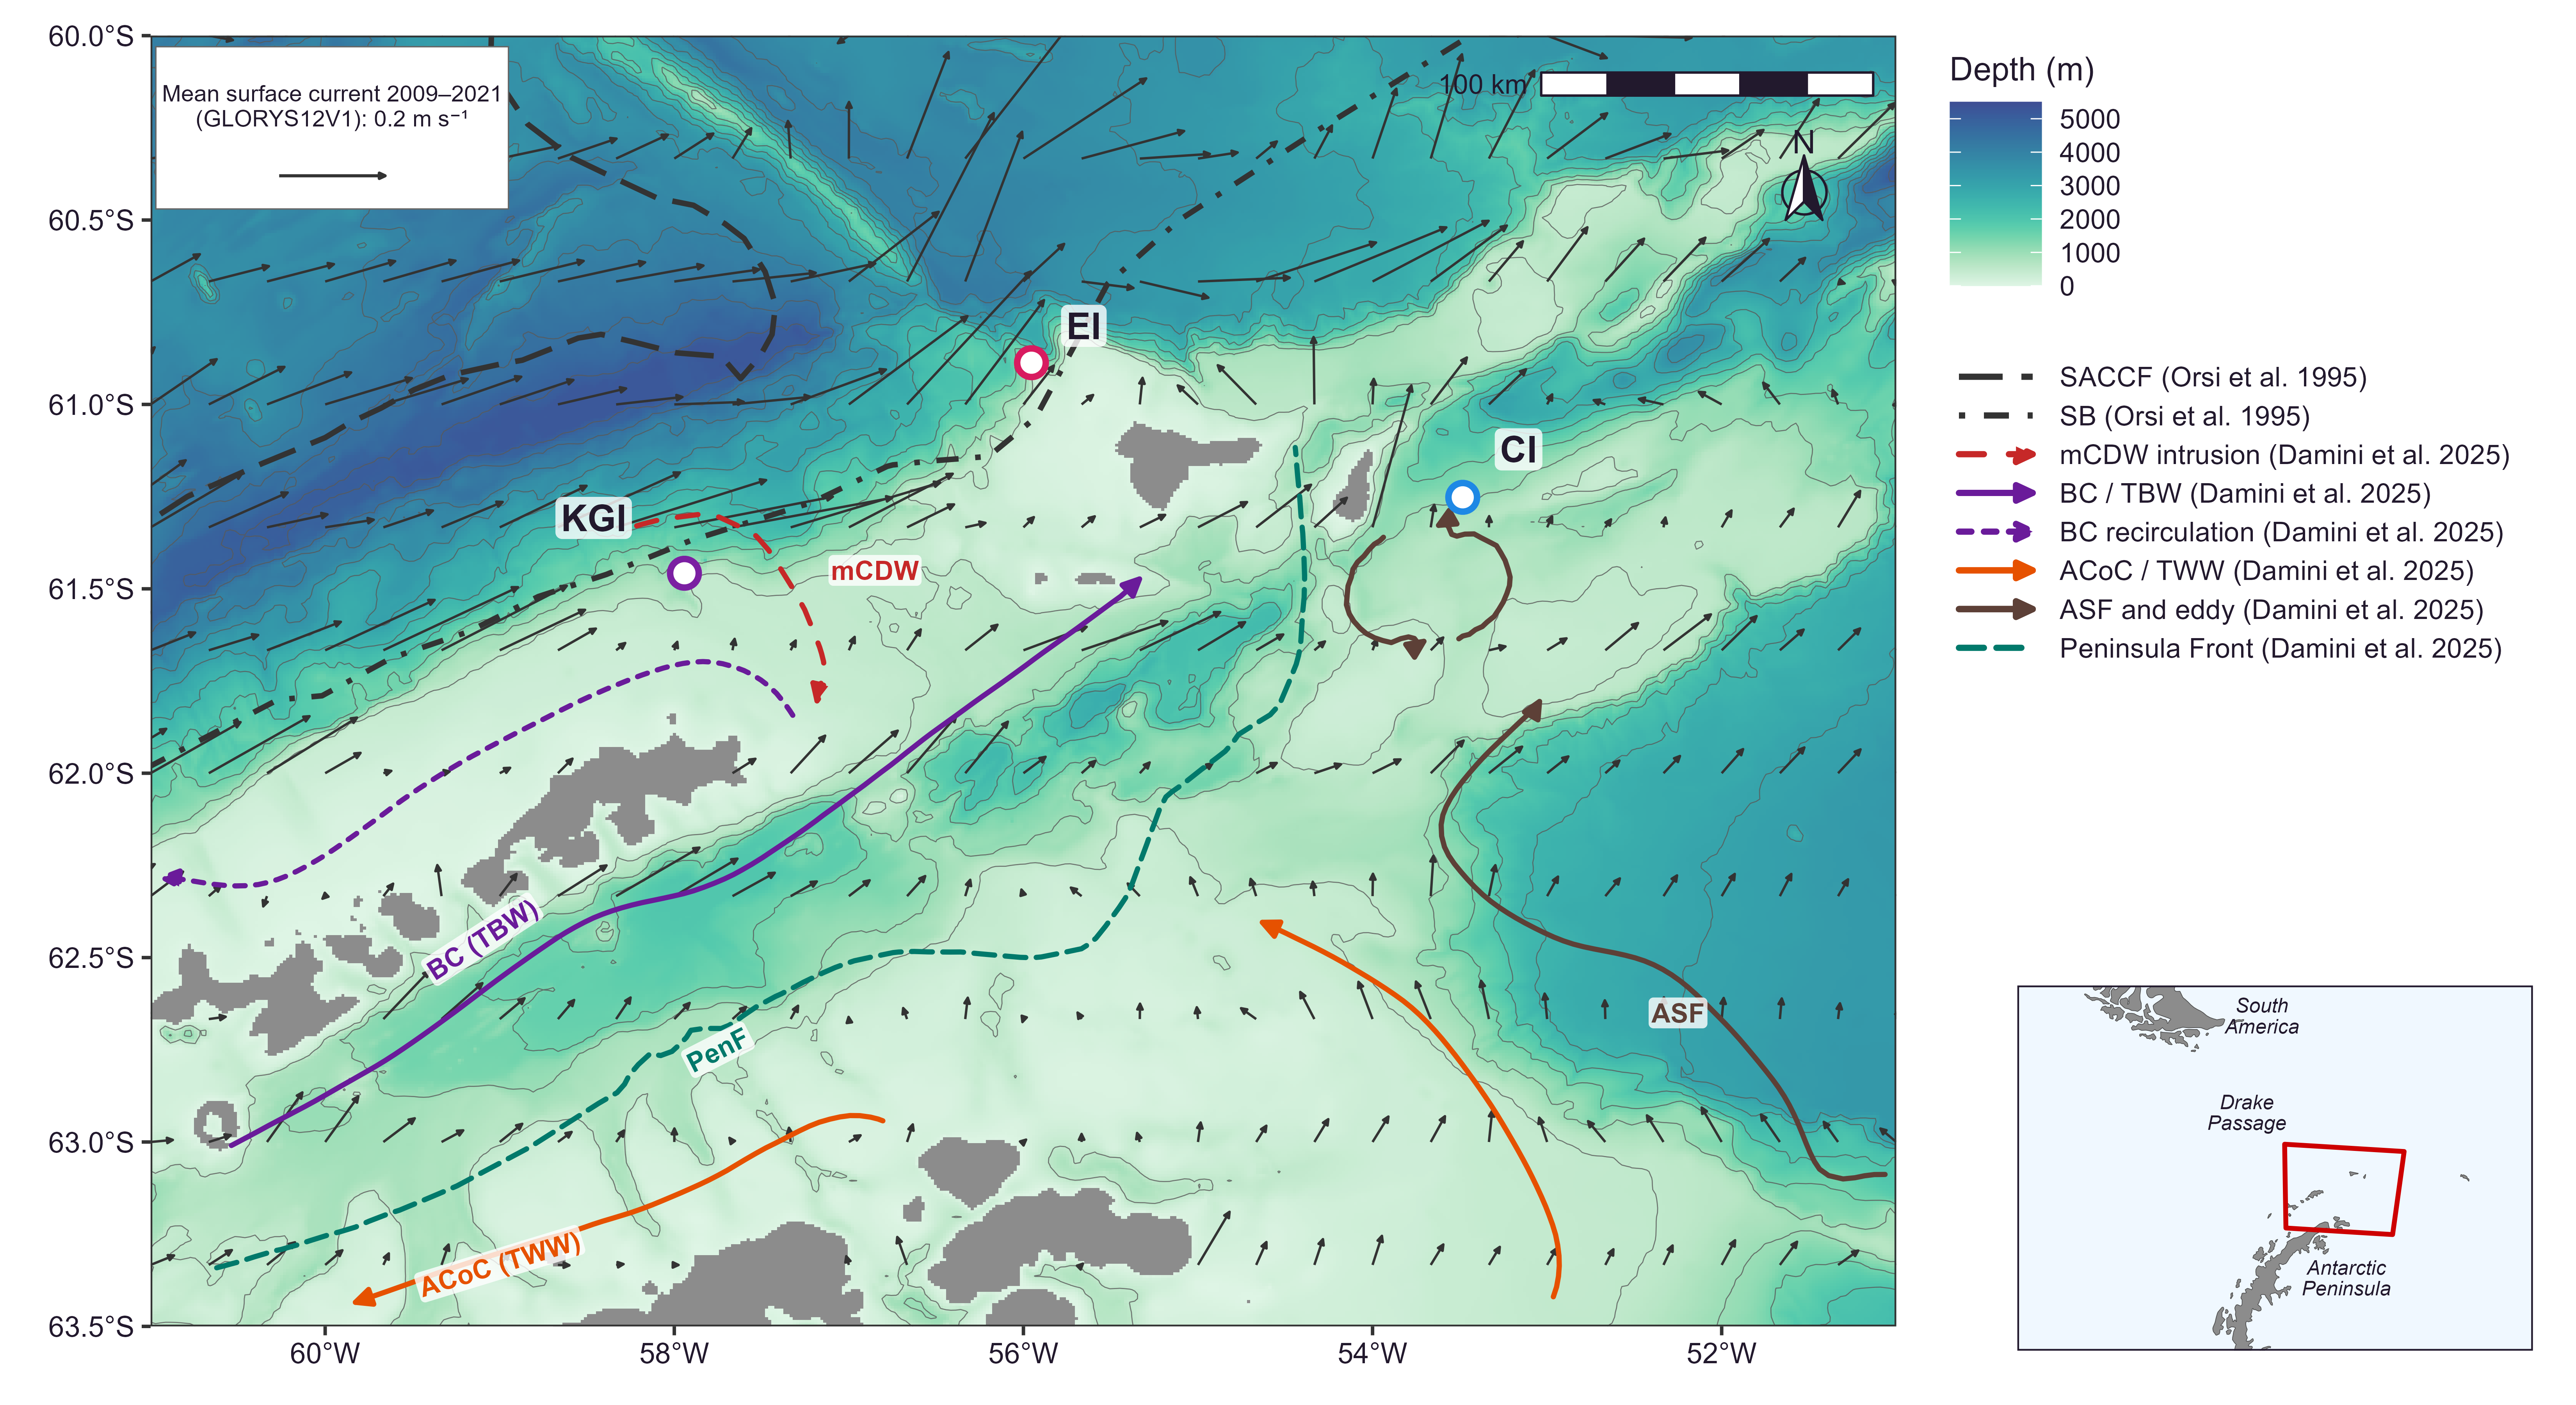
\includegraphics[width=1\linewidth,height=\textheight,keepaspectratio]{../outputs/01_study_area/study_area_currents_map_schematic.png}

}

\caption{\label{fig-map}Study area and regional circulation around the
South Shetland Islands, Antarctica. Circles mark the High-frequency
Acoustic Recording Package (HARP) sites at Elephant Island (EI; 2014),
King George Island (KGI; 2015--2016), and Clarence Island (CI; 2016),
shown on GMRT bathymetry (v4.4.1; Ryan et al.~2009) with 500-m isobaths.
Black arrows show mean surface currents for 2009--2021 from the
Copernicus Marine Service global ocean physics reanalysis (GLORYS12V1).
Black dashed and dot-dashed lines mark the Southern Antarctic
Circumpolar Current Front (SACCF) and the Southern Boundary of the
Antarctic Circumpolar Current (SB), respectively (Orsi et al.~1995).
Colored lines show schematic pathways digitized from Damini et
al.~(2025): intrusion of modified Circumpolar Deep Water (mCDW); the
Bransfield Current (BC), carrying Transitional Zonal Water with
Bellingshausen Sea influence (TBW), and its recirculation; the Antarctic
Coastal Current (ACoC), carrying Transitional Zonal Water with Weddell
Sea influence (TWW); the Antarctic Slope Front (ASF) and associated
eddy; and the Peninsula Front (PenF). The inset shows the location of
the study area (red box) relative to the Antarctic Peninsula and South
America.}

\end{figure}%

\subsection{Water-column structure}\label{sec-water}

To describe the water column at each site, daily potential temperature
and practical salinity were taken from the Copernicus Marine Service
global ocean physics reanalysis (GLOBAL\_MULTIYEAR\_PHY\_001\_030,
dataset version 202311; 1/12°, daily means), and daily dissolved oxygen
was taken from the companion global biogeochemistry hindcast
(GLOBAL\_MULTIYEAR\_BGC\_001\_029, dataset version 202406; 1/4°, daily
means), both accessed 17--18 November 2026 (Section~\ref{sec-env}). Each
variable was averaged over all ocean grid cells within a ±20 km box
centered on each site, at every model level from the surface (0.5 m) to
1000 m. Because the shelf slope runs through each box, only part of the
box reaches the deeper levels, so deep means represent only the cells
deep enough to contain those levels. Oxygen was unavailable below the
deepest water in the coarser biogeochemistry box (773 m at KGI, 1046 m
at CI).

We divided the upper 1000 m into three layers, used both to describe the
water column and to define the habitat predictors
(Section~\ref{sec-stats}): a surface layer (0--100 m), a mid-water layer
(100--500 m), and a deep layer (500--1000 m). The boundaries were
derived from the reanalysis using depth-constrained clustering of
temperature--salinity anomalies and water-mass features of the mean
profiles (Supplement S1; Figure~\ref{fig-layers}).

Daily profiles were linearly interpolated onto a regular grid in the
square root of depth (300 levels, no extrapolation) and displayed as one
continuous depth--time section from January 2014 to December 2016
(Figure~\ref{fig-sections}). Each period used the box of the site that
was recording, or about to record, in that period: EI for 2014, KGI for
January 2015 -- January 2016, and CI for February -- December 2016.
Sea-ice concentration from the same reanalysis and box
(Section~\ref{sec-ice}) was shown above the sections. Layer-mean
temperature, salinity, oxygen and eddy kinetic energy were summarized as
the mean ± SD over each site's recording period (Table S\ins{INSERT}).
Temperature--salinity diagrams for each site's recording period were
plotted with contours of potential density anomaly (\(\sigma_\theta\))
calculated at zero pressure using the UNESCO EOS-80 equation of state
(oce R package 1.8-3; Kelley \& Richards 2024) (Figure~\ref{fig-ts}).

\begin{figure}[htbp]

\centering{

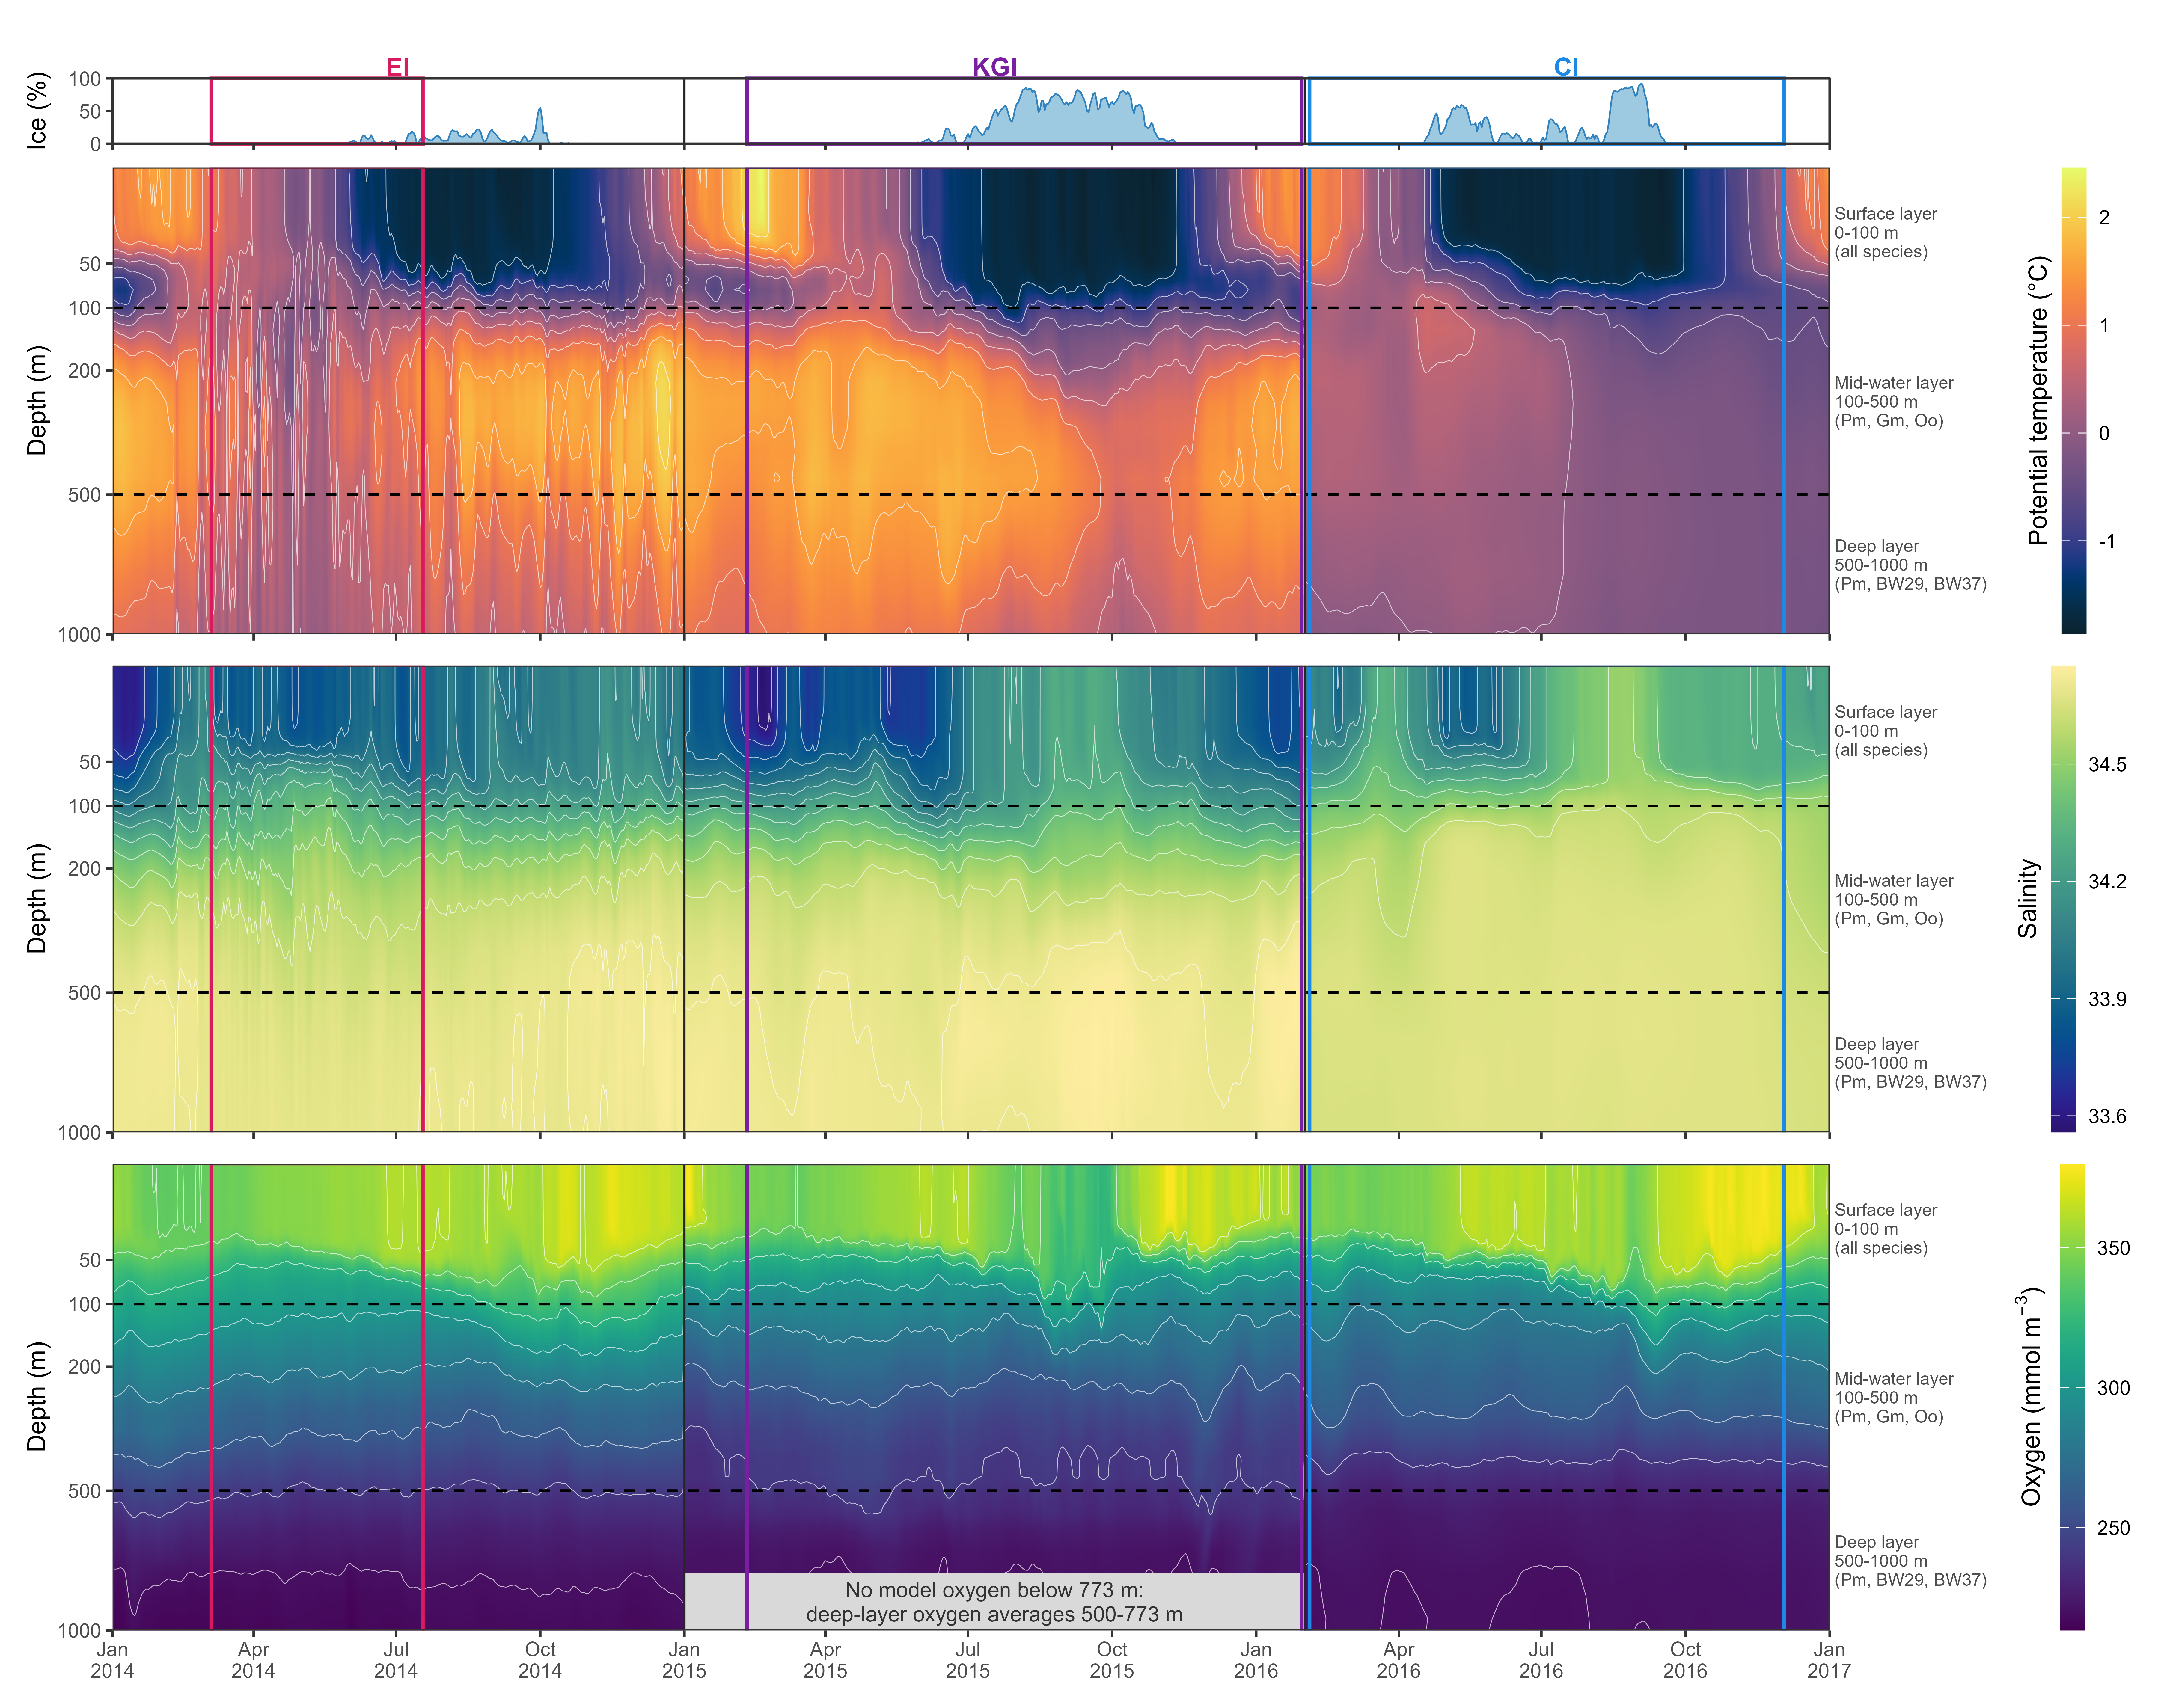
\includegraphics[width=1\linewidth,height=\textheight,keepaspectratio]{../outputs/02_deep_oceanography/ts_sections.png}

}

\caption{\label{fig-sections}Daily water-column conditions from January
2014 to December 2016 in the upper 1000 m. The record is assembled from
the ±20 km box around EI (2014), KGI (January 2015 -- January 2016), and
CI (February -- December 2016). Thin vertical black lines mark where the
source site changes, and colored outlines mark each site's recording
period. Top: sea-ice concentration (\%). Lower panels: potential
temperature (°C), salinity, and dissolved oxygen (mmol m\(^{-3}\)) from
the Copernicus Marine Service global physics reanalysis (temperature,
salinity; 1/12°) and biogeochemistry hindcast (oxygen; 1/4°), plotted on
a square-root depth axis with white contours (0.5 °C, 0.1, and 20 mmol
m\(^{-3}\), respectively). Dashed lines mark the boundaries of the
surface (0--100 m), mid-water (100--500 m) and deep (500--1000 m)
layers; right-hand labels give the species whose foraging depths fall in
each layer (Pm, sperm whale; Gm, long-finned pilot whale; Oo, killer
whale; BW29, southern bottlenose whale; BW37, BW37 beaked whale). Grey
areas mark depths with no model water in the box; at KGI, oxygen is
unavailable below 773 m, so the deep-layer oxygen mean there covers
500--773 m.}

\end{figure}%

\subsection{Sea ice}\label{sec-ice}

Daily sea-ice concentration was obtained from the Copernicus Marine
Service global ocean physics reanalysis
(GLOBAL\_MULTIYEAR\_PHY\_001\_030, dataset version 202311; 1/12°
horizontal resolution; accessed 17--18 November 2026) and averaged over
a box extending ±20 km from each HARP (approximately 40 × 40 km). The
product reports open-water ocean cells as missing rather than zero.
These cells were therefore set to zero before averaging, so the daily
box mean is the fraction of the whole box covered by ice, not the mean
concentration of the ice-covered cells only.

Acoustic occurrence was first described across sea-ice conditions as the
percentage of time bins with detections in four sea-ice concentration
classes (0--5, 5--15, 15--50 and \textgreater50\%;
Figure~\ref{fig-iceocc}). Sea ice was then used in two ways in the
models. First, for each species and site, acoustic presence was modeled
against sea-ice concentration using all recording bins
(Section~\ref{sec-stats}), to describe how occurrence varied with the
seasonal advance and retreat of the ice. Second, the habitat models
(Section~\ref{sec-stats}) were meant to test the influence of other
environmental conditions only when each species could plausibly be
present. They were therefore restricted, for each species, to time bins
whose mean sea-ice concentration was no greater than the highest
bin-mean concentration at which that species was detected, pooled across
sites. The cutoffs were 88.9\% for killer whales, 84.5\% for sperm
whales, 33.4\% for long-finned pilot whales, and 12.6\% for southern
bottlenose whales and 12.6\% for BW37 beaked whales (Table
\ref{tab:icecut}). By construction, no bins with detections were
excluded. The restriction removed no bins at EI. It removed 1 of 152
two-day bins for killer whales at CI, 12 of 76 (CI) and 25 of 89 (KGI)
four-day bins for long-finned pilot whales, and 24 of 76 (CI) and 33 of
89 (KGI) four-day bins for each beaked whale. Sea-ice concentration was
therefore not a candidate predictor in the habitat models.

\subsection{Acoustic detection}\label{sec-detect}

For beaked whales, sperm whales (\emph{Physeter macrocephalus}), and
long-finned pilot whales (\emph{Globicephala melas}), echolocation
signals were first detected with an expert system using a two-step
approach (Roch et al.~2011) and then verified by an expert analyst. For
beaked whales at EI, a previously published dataset of echolocation
signals was used (Baumann-Pickering et al.~2015); the same data
processing methods were replicated for beaked whales at KGI and CI, and
for sperm whale and long-finned pilot whale signals at all sites. Killer
whale (\emph{Orcinus orca}) signals were identified by an expert analyst
through manual review of long-term spectral averages (LTSAs)
\conf{method and LTSA settings}. Beaked whale echolocation pulses were
classified into southern bottlenose whale (\emph{Hyperoodon planifrons};
BW29) and the BW37 and BW58 signal types. Previous work has hypothesized
that the BW37 and BW58 echolocation pulses could be produced by Gray's
(\emph{Mesoplodon grayi}) and strap-toothed (\emph{M. layardii}) beaked
whales, respectively (Trickey et al.~2015, Baumann-Pickering et
al.~2015, Barlow et al.~2021); Shepherd's beaked whale (\emph{Tasmacetus
shepherdi}) has also been proposed as a candidate for these unidentified
signals (Barlow et al.~2021). Further research is still needed to
confirm the species producing these echolocation pulses.

Only echolocation clicks were used to define presence; sperm whale slow
clicks (n = 44 events) and killer whale high-frequency modulated signals
(n = 3 events) were excluded. Verified detections were summarized into
5-min bins, and a bin was considered positive for a species if any
detection overlapped it. Daily acoustic presence was quantified as the
number of minutes in positive bins per day (positive bins × 5 min).
Daily recording effort was calculated as the time within each
deployment's recording period, accounting for partial first and last
days and for the duty cycle at EI and KGI.

To assess whether duty cycling reduced detectability, the continuously
recorded CI data were subsampled to the EI (5 min on every 6 min) and
KGI (10 min on every 13.33 min) duty cycles at 100 random phase offsets,
and the proportion of detection events, positive 5-min bins, and
presence days retained was calculated for each species (Table
\ref{tab:duty}; Figure~\ref{fig-duty}). Subsampling retained ≥ 89.6\% of
positive 5-min bins and ≥ 89.6\% of presence days on average for all
species under either duty cycle (lowest: sperm whales under the KGI duty
cycle; ≥ 96.5\% of presence days for all other species), despite
recording only 83.3\% (EI) and 75.0\% (KGI) of the time. Because losses
were far smaller than proportional to recording time, presence was not
scaled by recording effort.

\subsection{Environmental data}\label{sec-env}

Environmental conditions at each site were characterized with daily
output from the Copernicus Marine Service global ocean physics
reanalysis (GLOBAL\_MULTIYEAR\_PHY\_001\_030, GLORYS12V1, dataset
version 202311; 1/12° horizontal resolution, 50 vertical levels) and
global biogeochemistry hindcast (GLOBAL\_MULTIYEAR\_BGC\_001\_029,
dataset version 202406; 1/4° resolution), both accessed 17--18 November
2026 \ins{REF product DOIs}. From the physics reanalysis, we used
potential temperature, zonal and meridional velocity, mixed layer depth,
and sea-ice concentration (Section~\ref{sec-ice}). Mixed layer depth is
defined in this product as the depth at which density exceeds its value
at 10 m by the amount equivalent to a 0.2 °C temperature decrease under
local surface conditions. From the biogeochemistry hindcast, we used
chlorophyll-\emph{a}. Following \ins{COMPANION PAPER}, fronts and
surface mesoscale stirring were described with backward-in-time
finite-size Lyapunov exponents (FSLEs) and the orientations of the
associated finite-size Lyapunov vectors (FSLVs) (d'Ovidio et al.~2004),
from the AVISO+ FSLE product computed from DUACS delayed-time
multi-satellite absolute geostrophic velocities (version DT2024; 1/25°,
daily; accessed 17--18 November 2026) \ins{REF AVISO+}.

Each variable was averaged daily over all ocean grid cells within ±20 km
of each recorder (approximately 40 × 40 km). This area is larger than
the distances over which the target species' echolocation clicks can be
detected by a HARP: up to about 4 km for beaked whales (Zimmer et
al.~2008, Hildebrand et al.~2015), \ins{range, with reference} for
killer whales and long-finned pilot whales, and up to about 20 km for
sperm whales, which at these latitudes are adult males \ins{REF}. It
therefore includes the water around any detected animal. The box was
also large enough to contain several grid cells of the coarser 1/4°
biogeochemistry product (one cell spans \textasciitilde28 km in
latitude), whereas a ±10 km box would contain at most one. The ±20 km
box contained 32--45 physics cells (EI 32, KGI 36, CI 45) and 3--6
biogeochemistry cells (EI 6, KGI 3, CI 3) at the surface.

Water-column variables were averaged over the three depth layers:
surface (0--100 m), mid-water (100--500 m), and deep (500--1000 m). Each
layer mean was weighted by thickness: each model level represents the
depth interval between the midpoints to its neighbouring levels, and its
weight is the overlap of that interval with the layer. Only grid cells
with water at a level contributed, so deep-layer means represent the
parts of the box deep enough to reach them. Eddy kinetic energy (EKE)
was calculated at each model level as \(\frac{1}{2}(u'^2 + v'^2)\),
where \(u'\) and \(v'\) are the daily box-mean velocity components minus
their 10-year means at that site and level, and then averaged over the
mid-water and deep layers in the same way. Because a box mean over fewer
grid cells averages out less of the eddy variability, absolute EKE
values are not directly comparable between layers or sites (e.g., at EI,
deep-layer EKE exceeded surface EKE); within a site and layer, its
variation over time is comparable.

Mean FSLE included grid cells with an FSLE of zero, where the
particle-separation threshold was not reached within the integration
time; these zeros are valid values, not missing data. FSLV orientation
is axial (orientations 180° apart describe the same front), so it was
averaged by doubling the angles, taking the circular mean, and halving
the result, using only the cells with nonzero FSLE (on average 87--95\%
of the box per day). To represent the delayed response of odontocete
prey to phytoplankton production, surface chlorophyll-\emph{a} was
averaged over the 30-day window ending 3 months before each day.

All variables were extracted for each site's deployment years ± 5 years
(EI 2009--2019, KGI 2010--2021, CI 2011--2021). This 10-year record
provided the climatologies used to deseason predictors
(Section~\ref{sec-stats}) and the reference mean flow for EKE, and it
allowed lagged chlorophyll-\emph{a} to be calculated for the first
months of each deployment. No predictor had missing values on any
recording day.

\subsubsection{Model comparison and validation}\label{sec-valid}

To assess how much the water-column predictors depended on the choice of
ocean model, and how well they reproduced observations, the Copernicus
reanalysis was compared with an independent ocean model and with
satellite and in-situ observations. HYCOM GOFS 3.1 (GLBv0.08; 1/12° ×
1/25°, 40 depth levels) \ins{REF} daily temperature and salinity were
obtained for each site's recording period, using the 3-hourly time step
closest to 12:00 UTC. No single HYCOM experiment spans 2014--2016, so
the reanalysis (experiment 53.X) was used for 2014 and the analysis
experiments 56.3 and 57.2 thereafter. Daily sea surface temperature from
the Aqua MODIS sensor (4 km, daytime, quality-masked; NOAA CoastWatch
ERDDAP dataset erdMH1sstd1dayR20190SQ) \ins{REF} was used where at least
20\% of the box's ocean pixels were valid. All products were averaged
over the same ±20 km box around each site and matched by date. HYCOM was
interpolated to the Copernicus model levels, and agreement was
summarized as the mean difference (bias), root-mean-square error (RMSE)
and Pearson correlation (\(r\)), for raw values and for anomalies from
each product's monthly means over the matched days
(Figure~\ref{fig-hycom}).

Both models were also compared with in-situ profiles from the World
Ocean Database \ins{REF} in a wider region around the sites (60--63°S,
52--60°W) from 2014 to 2016: 915 profiles from instrumented seals, Argo
floats, ship CTDs, bottle casts and expendable bathythermographs
(Figure~\ref{fig-insitu} a). Only observations and profiles that passed
the World Ocean Database quality control were used. For each profile,
both models were sampled at the nearest grid cell with water on the
profile's day (Copernicus daily mean; HYCOM time step nearest the
profile time). Observed profiles were interpolated to the Copernicus
model levels within their measured depth range, and oxygen was converted
from µmol kg\(^{-1}\) to mmol m\(^{-3}\) using in-situ density. Bias,
RMSE and \(r\) were computed at each level and for thickness-weighted
means of the three depth layers, using only profiles covering at least
80\% of a layer and only profile--level combinations available in both
models. Because both models assimilate some in-situ profiles (e.g.,
Argo), this comparison is not fully independent.

\subsection{Statistical analyses}\label{sec-stats}

Relationships between odontocete acoustic presence and environmental
conditions were modeled with generalized additive models (GAMs),
consistent with the methods described for baleen whales in
\ins{COMPANION PAPER}. Separate models were fit for each species at each
site. To reduce temporal autocorrelation, daily presence was aggregated
into consecutive multi-day bins. For each species and site, a GAM of
daily presence minutes on a smooth of days since the start of recording
was fit, and the bin length was the first lag at which the
autocorrelation of its residuals fell within the 95\% confidence bounds.
For comparability across sites, each species was assigned the longest
bin length among its sites, capped at 4 days to retain at least 30 bins
at the shortest deployment (EI, 135 days). Bins were 4 days long for all
species except killer whales (2 days); the cap applied to sperm whales,
southern bottlenose whales, and BW37, whose residual autocorrelation
lasted 6, 11, and 17 days, respectively. The response was the mean daily
presence minutes within each bin. Species--site combinations with fewer
than 10 bins containing detections were not modeled and are described
only in Section~\ref{sec-occ} (sperm whales at KGI, killer whales at EI
and KGI, and BW37 at CI). Models with 10--20 bins with detections
(long-finned pilot whales at EI, KGI, and CI, killer whales at CI,
southern bottlenose whales at KGI, and BW37 at EI) were identified as
low-sample models.

Two types of model were fit. Sea-ice models related presence to sea-ice
concentration alone, using all bins, and describe the seasonal pattern
of occurrence; because their residuals were strongly autocorrelated,
they are reported in the supplement, and occurrence across sea-ice
classes is presented descriptively in the main text
(Section~\ref{sec-ice}). Habitat models related presence to the
remaining environmental predictors, using only bins with sea-ice
concentration no greater than the highest concentration at which the
species was detected (Section~\ref{sec-ice}). Because the seasonal
pattern is described by the sea-ice models, the habitat models were
designed to test responses to conditions that were unusual for the time
of year. All habitat predictors with a seasonal cycle were therefore
expressed as anomalies from a 10-year climatology (deployment years ± 5
years): the 12 monthly means were interpolated to daily values with a
periodic cubic spline and subtracted from the daily values. EKE, FSLE
and FSLV orientation have almost no seasonal cycle (the seasonal cycle
explained ≤ 8\% of their daily variance at every site) and were used as
raw values.

Each candidate habitat predictor represents a different process (Table
\ref{tab:pred}). Water-column conditions were represented by the
temperature anomaly of each depth layer the species uses: the surface
layer (0--100 m) for all species, plus the mid-water layer (100--500 m)
for sperm and killer whales and the deep layer (500--1000 m) for sperm
whales, long-finned pilot whales, southern bottlenose whales and BW37,
according to their foraging depths (Table S\ins{INSERT}). Temperature
was the only water-mass variable because, of the variables available, it
was the one the reanalysis reproduced well in all three layers when
compared with in-situ profiles (Section~\ref{sec-valid}; \(r\) =
0.74--0.89 for layer means, versus 0.19 for mid-water salinity and ≤
0.15 for oxygen). Eddy activity was represented by EKE in the mid-water
and deep layers used by each species, and surface fronts by FSLE and
FSLV orientation. Stratification was represented by the mixed layer
depth anomaly. Productivity was represented by the anomaly of
log\(_{10}\)-transformed surface chlorophyll-\emph{a} averaged over the
30-day window ending 3 months before each day. A single lag was used for
all species: among the candidate lags, the 3-month lag was the most
consistently associated with presence in exploratory single-term models
(significant in 9 of 11 species--site models, versus 6 of 11 for a
5-month lag).

All models used a Tweedie distribution with a log link (power parameter
estimated between 1.1 and 1.9), smoothing parameters estimated by
restricted maximum likelihood (REML), and thin-plate regression splines
with a basis dimension of 4. FSLV orientation was fit with a cyclic
cubic spline joined at ±90°, because orientations differing by 180° are
equivalent (Haller 2015). For each species and site, the candidates were
screened for collinearity by sequentially removing the predictor with
the highest variance inflation factor (VIF) until all were ≤ 5 (Zuur et
al.~2010), and terms were then removed by backward selection, using
additional shrinkage of smooth terms (\texttt{select\ =\ TRUE}), until
all remaining terms were significant (\(p\) ≤ 0.05). To limit
overfitting, the number of smooth terms was restricted following the
guideline of at least 10 observations per estimated term (Peduzzi et
al.~1996, Harrell 2015) \conf{references}. Each model was allowed at
most one term per 10 bins; in low-sample models (10--20 bins with
detections), where the bins with detections rather than all bins carry
most of the information, at most two terms were allowed (i.e., about one
term per 10 bins with detections). The limit was applied during backward
selection: once all remaining terms were significant, the least
significant term continued to be removed until the model met the limit.
With shrinkage, smooth terms in the final models had a median of 1.6
effective degrees of freedom (range 0.8--2.8). A common set of
predictors was then chosen for each species (the predictors selected at
any of its sites), and the final model at each site was refit from this
set with the same backward selection.

Model fit was assessed with residual diagnostics, basis-dimension checks
and concurvity (Table \ref{tab:diagnostics}). Residual autocorrelation
was tested with a Ljung--Box test over lags 1--5 bins, computed on the
bin series with bins removed by the ice filter treated as gaps. As a
sensitivity analysis, each final model was refit with an additional
first-order autoregressive (AR(1)) process in glmmTMB (Brooks et
al.~2017), keeping the same smooth terms (FSLV orientation as
\(\sin 2\theta\) and \(\cos 2\theta\)). AR(1) was retained where it
lowered AIC by more than 2, and each term was then tested by a
likelihood-ratio test (Supplement S5). Analyses were conducted in R
4.5.1 (R Core Team 2025) with the packages mgcv 1.9.3 (Wood 2017), car
3.1.3 (Fox \& Weisberg 2019), gratia 0.11.1 (Simpson 2024) and glmmTMB
1.1.15.2 (Brooks et al.~2017).

\begin{table}[!h]
\centering
\caption{\label{tab:pred}Candidate predictors for the habitat models. Layers: surface 0--100 m (all species); mid-water 100--500 m (sperm whale, killer whale); deep 500--1000 m (sperm whale, long-finned pilot whale, southern bottlenose whale, BW37). Sea-ice concentration (Copernicus PHY) was used only in the sea-ice models and for the ice cutoff.}
\centering
\fontsize{9}{11}\selectfont
\begin{tabular}[t]{>{\raggedright\arraybackslash}p{3.3cm}>{\raggedright\arraybackslash}p{3.4cm}>{\raggedright\arraybackslash}p{2.6cm}>{\raggedright\arraybackslash}p{1.8cm}>{\raggedright\arraybackslash}p{1.3cm}>{\raggedright\arraybackslash}p{2cm}}
\toprule
Predictor & Represents & Layer & Units & Form & Source\\
\midrule
Potential temperature & Water mass & Mean of each layer used & °C & Anomaly & Copernicus PHY\\
FSLE (backward-in-time) & Surface fronts and stirring & Surface & day⁻¹ & Raw & AVISO+\\
FSLV orientation (cyclic) & Orientation of surface fronts & Surface & ° & Raw & AVISO+\\
EKE, ½(u′² + v′²) & Eddy activity at foraging depth & Mid-water and/or deep & cm² s⁻² & Raw & Copernicus PHY\\
Mixed layer depth & Stratification & Surface & m & Anomaly & Copernicus PHY\\
log10 chlorophyll-a, 30-day mean ending 3 months earlier & Delayed productivity (prey) & Surface & log10 mg m⁻³ & Anomaly & Copernicus BGC\\
\bottomrule
\end{tabular}
\end{table}

\section{Results}\label{results}

\subsection{Acoustic occurrence}\label{sec-occ}

\ins{Occurrence text to be written (@fig-weekly; detection days per species and site)}

Occurrence differed strongly across sea-ice conditions
(Figure~\ref{fig-iceocc}). \ins{Text to be written}

Three species--site combinations had too few detections to model (killer
whales at EI and KGI, 3 detection days each; BW37 at CI, 11 days; Table
\ref{tab:rare}). Killer whale detections at KGI coincided with high eddy
kinetic energy in the mid-water and deep layers (94th--97th percentile
of recording days), and one of the three detections occurred under 70\%
sea-ice cover. BW37 at CI was detected only in ice-free periods
(March--April and November), on days with above-typical deep-layer eddy
kinetic energy (83rd percentile).

\begin{figure}[htbp]

\centering{

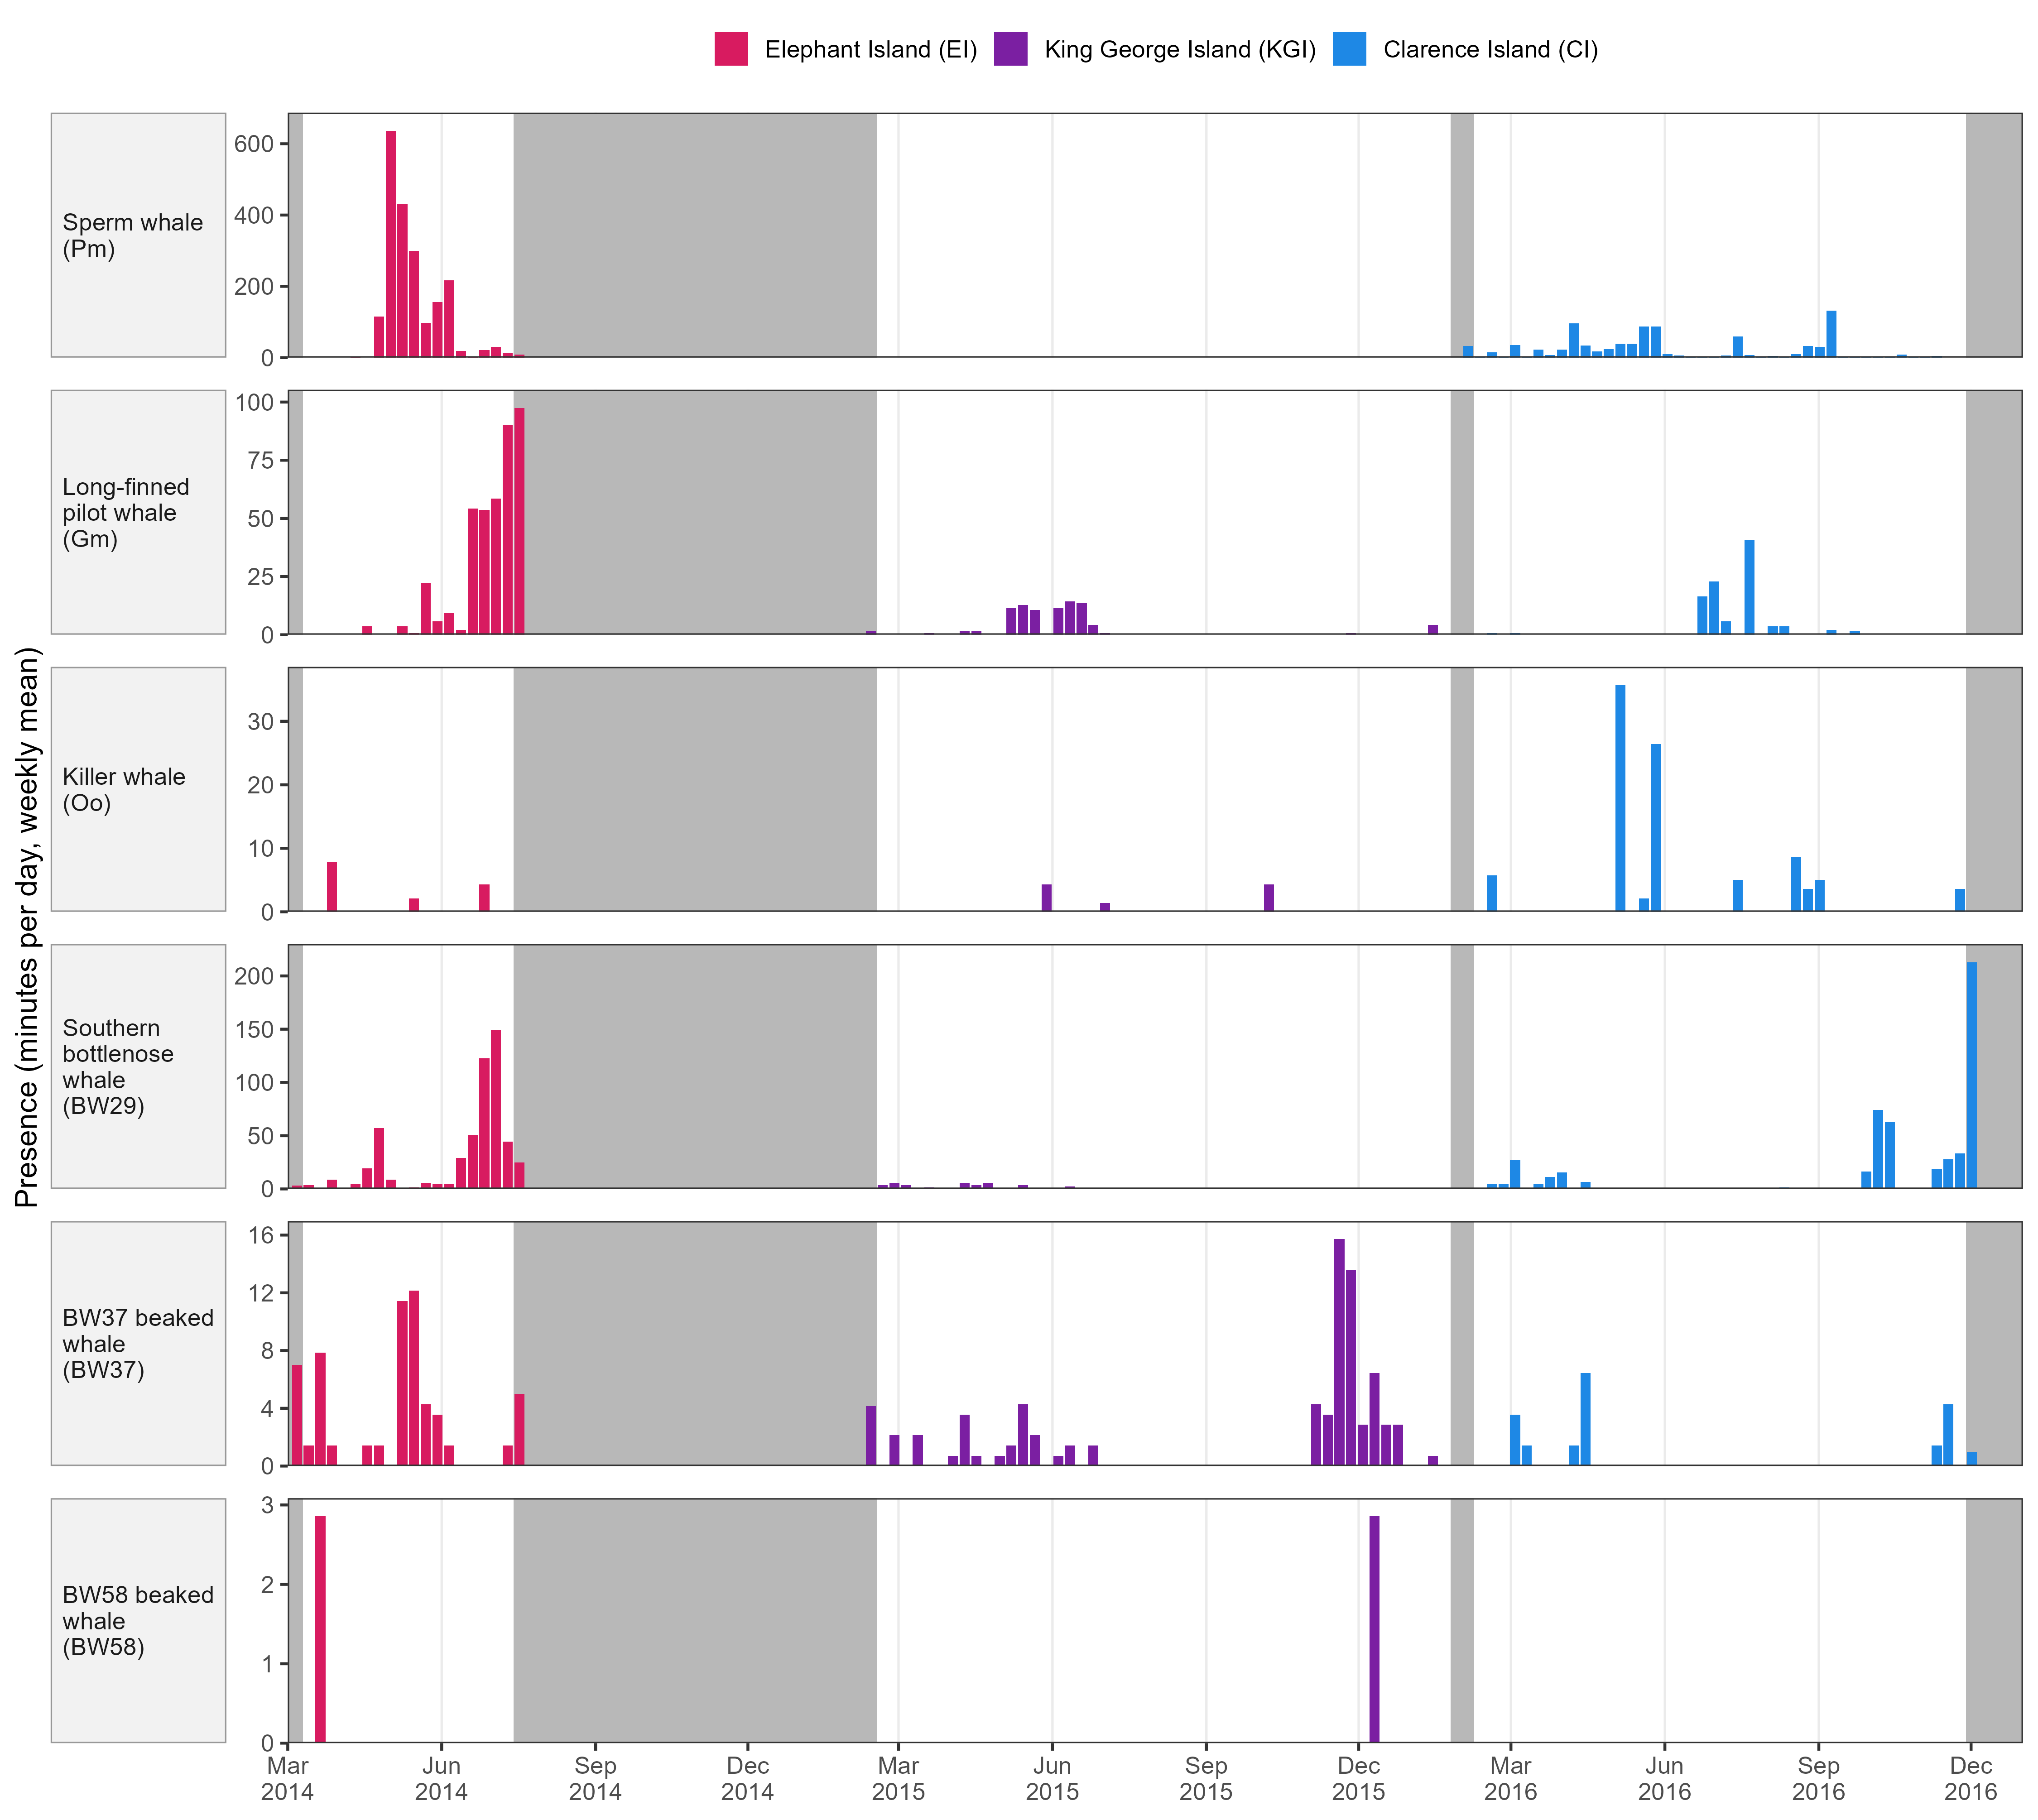
\includegraphics[width=1\linewidth,height=\textheight,keepaspectratio]{../outputs/07_results_occurrence/fig_weekly_presence.png}

}

\caption{\label{fig-weekly}Weekly acoustic presence of odontocetes at
EI, KGI and CI. \ins{Legend to be drafted}}

\end{figure}%

\begin{figure}[htbp]

\centering{

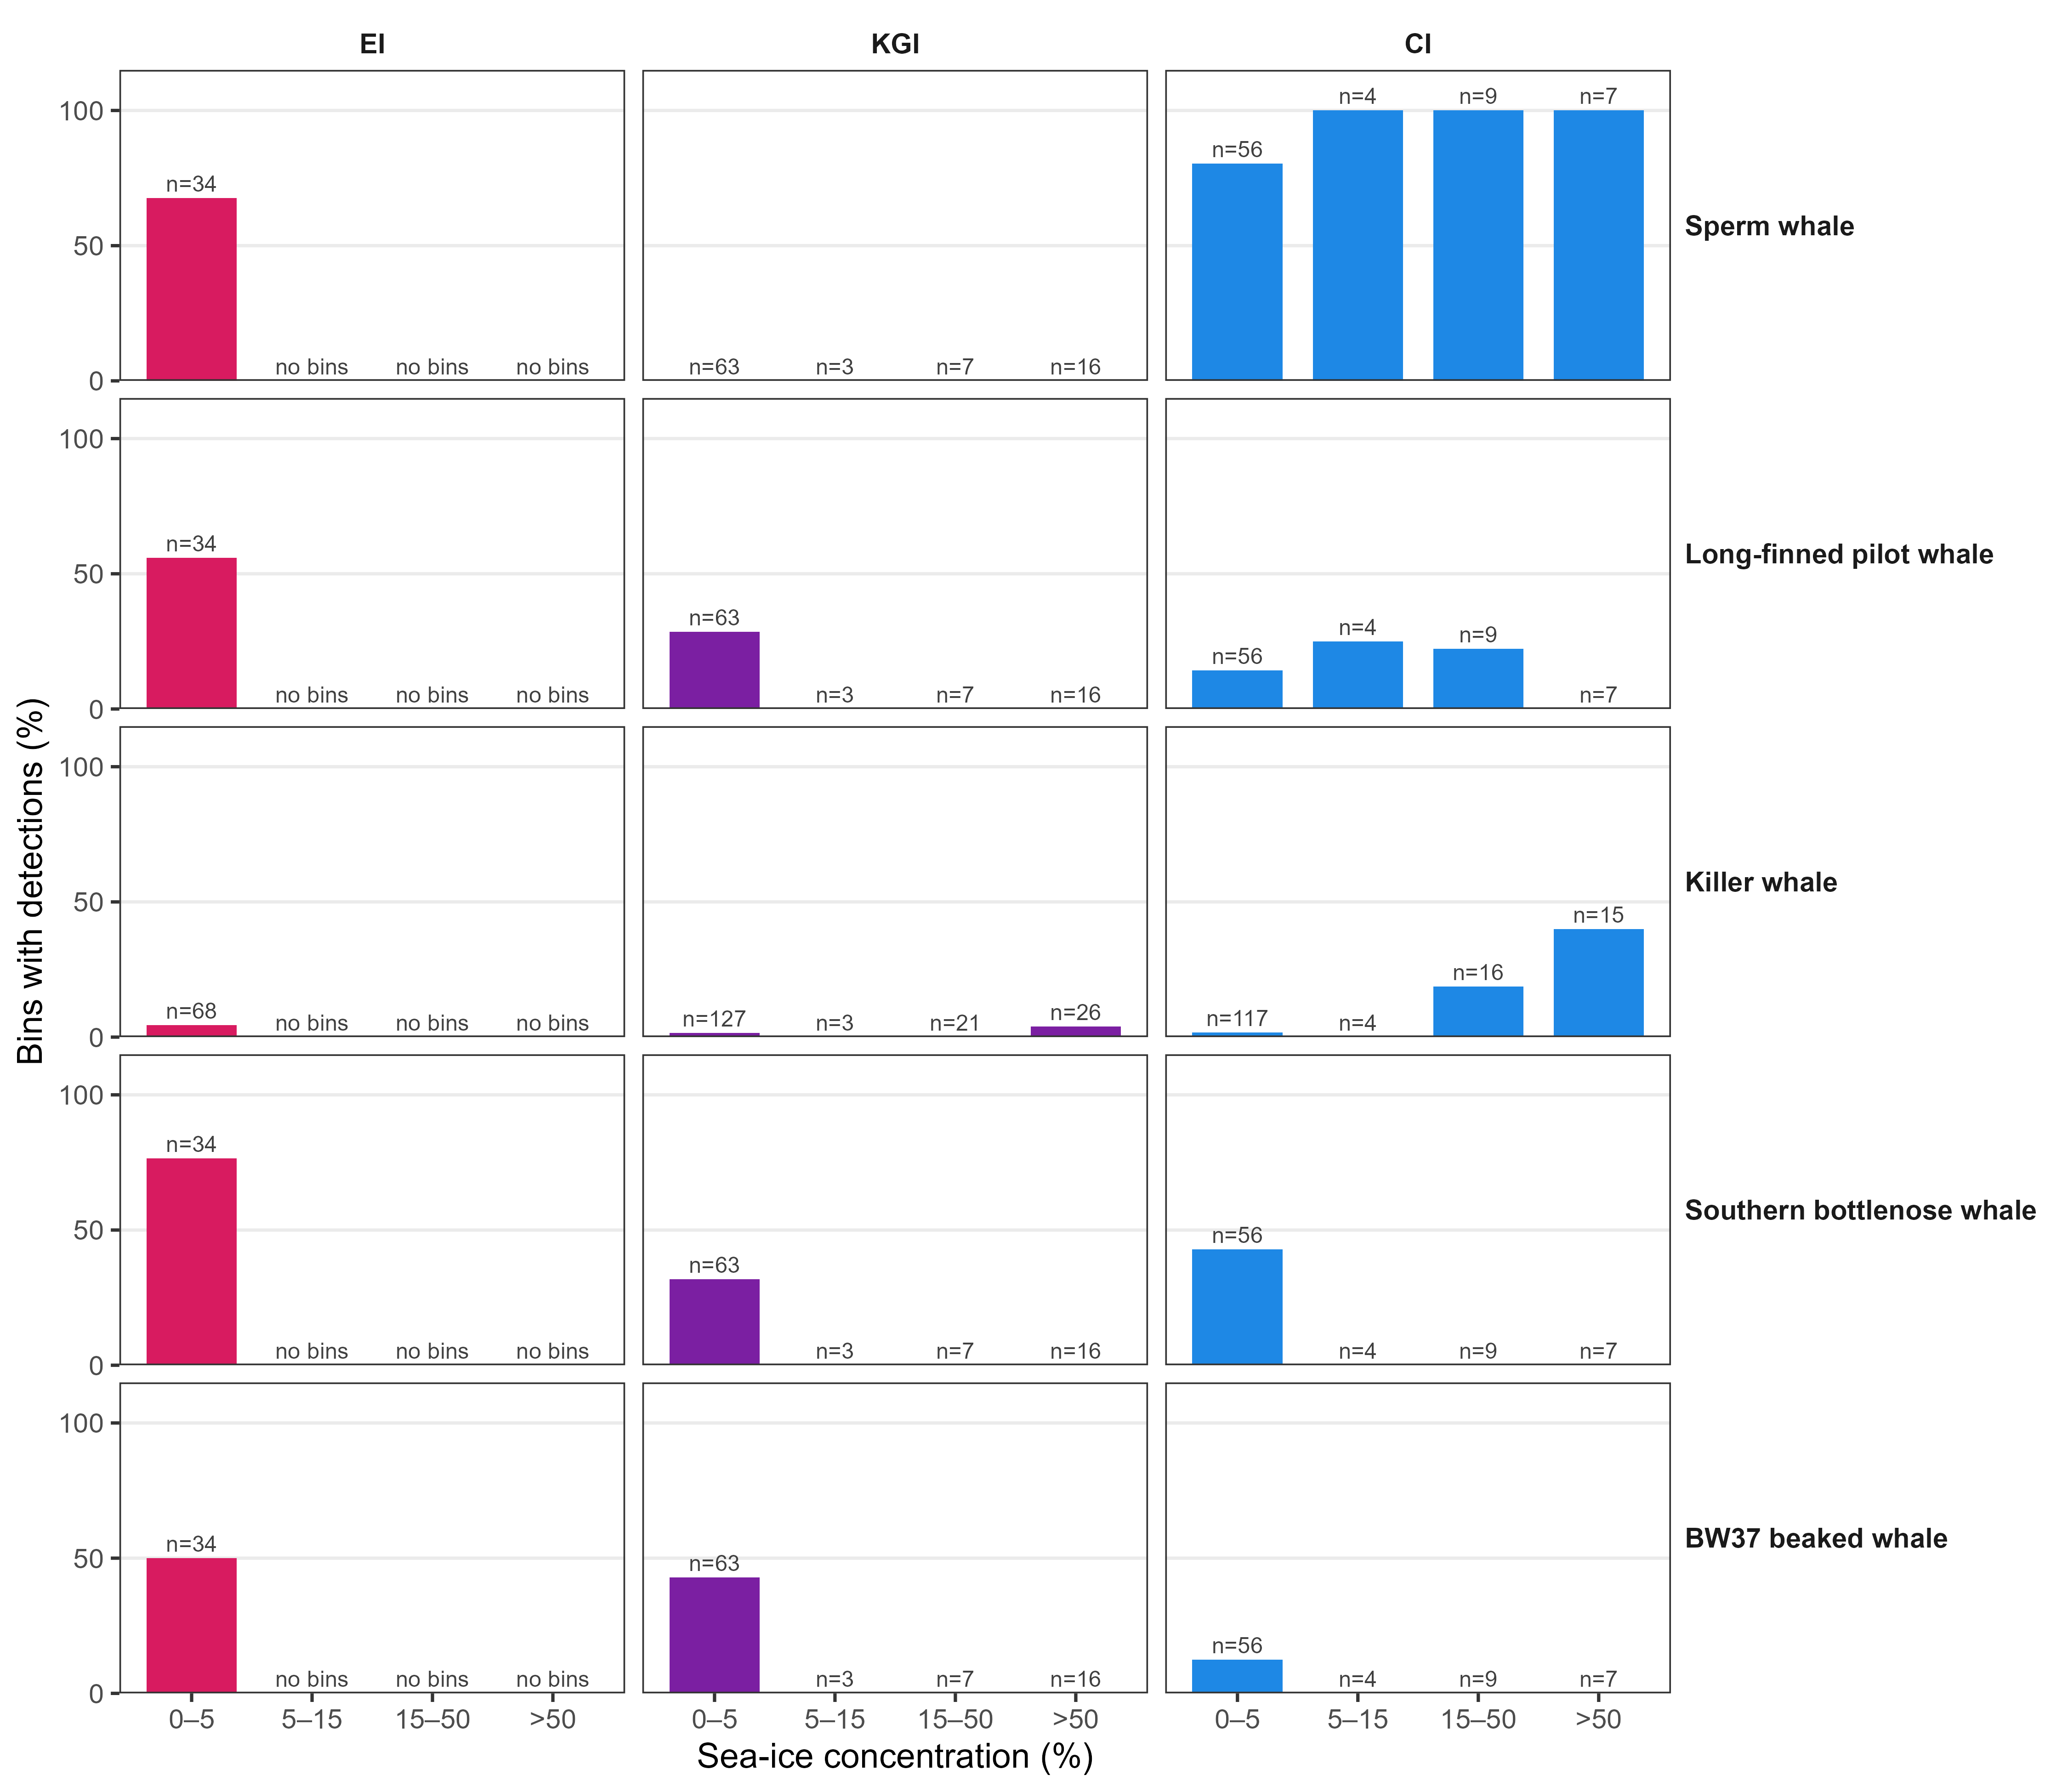
\includegraphics[width=1\linewidth,height=\textheight,keepaspectratio]{../outputs/08_results_gams/main_sea_ice_occurrence.png}

}

\caption{\label{fig-iceocc}Acoustic occurrence of odontocetes across
sea-ice conditions at Elephant Island (EI), King George Island (KGI) and
Clarence Island (CI): percentage of time bins with detections in each
sea-ice concentration class (Copernicus Marine Service reanalysis, mean
over the ±20 km box). Labels give the number of bins per class; ``no
bins'' indicates that the class did not occur during recording. Bins
were 4 days long (killer whales, 2 days).}

\end{figure}%

\subsection{Choice of ocean model}\label{choice-of-ocean-model}

The Copernicus reanalysis agreed with the independent observations at
least as well as HYCOM did, and it was used for all predictors. Against
MODIS surface temperature, Copernicus had smaller warm biases than HYCOM
at all sites (-0.01 to 0.18 °C vs 0.24 to 0.44 °C;
Figure~\ref{fig-hycom} a). At depth, the two models differed by a
near-constant offset, with HYCOM up to \textasciitilde1 °C warmer than
Copernicus at EI (Figure~\ref{fig-hycom} b). Against in-situ profiles,
Copernicus reproduced layer-mean temperature well in all three layers
(\(r\) = 0.89, 0.74 and 0.86 for the surface, mid-water and deep
layers), with smaller biases than HYCOM in the mid-water (0.20 vs 0.38
°C) and deep layers (0.02 vs 0.19 °C) and similar skill at the surface
(Figure~\ref{fig-insitu} b). In contrast, Copernicus mid-water salinity
was poorly reproduced (\(r\) = 0.19; HYCOM \(r\) = 0.52), and Copernicus
oxygen showed no positive correlation with observations below the
surface layer. Copernicus also provides sea-ice concentration, mixed
layer depth and a matching biogeochemistry hindcast from one consistent
multi-year system, whereas no single HYCOM experiment covered the study
period. Temperature was therefore used as the only water-mass variable
in the habitat models (Section~\ref{sec-stats}).

\subsection{Habitat models}\label{habitat-models}

\ins{Results text to be written (Table \ref{tab:habitat}; @fig-curves)}

\begin{figure}[htbp]

\centering{

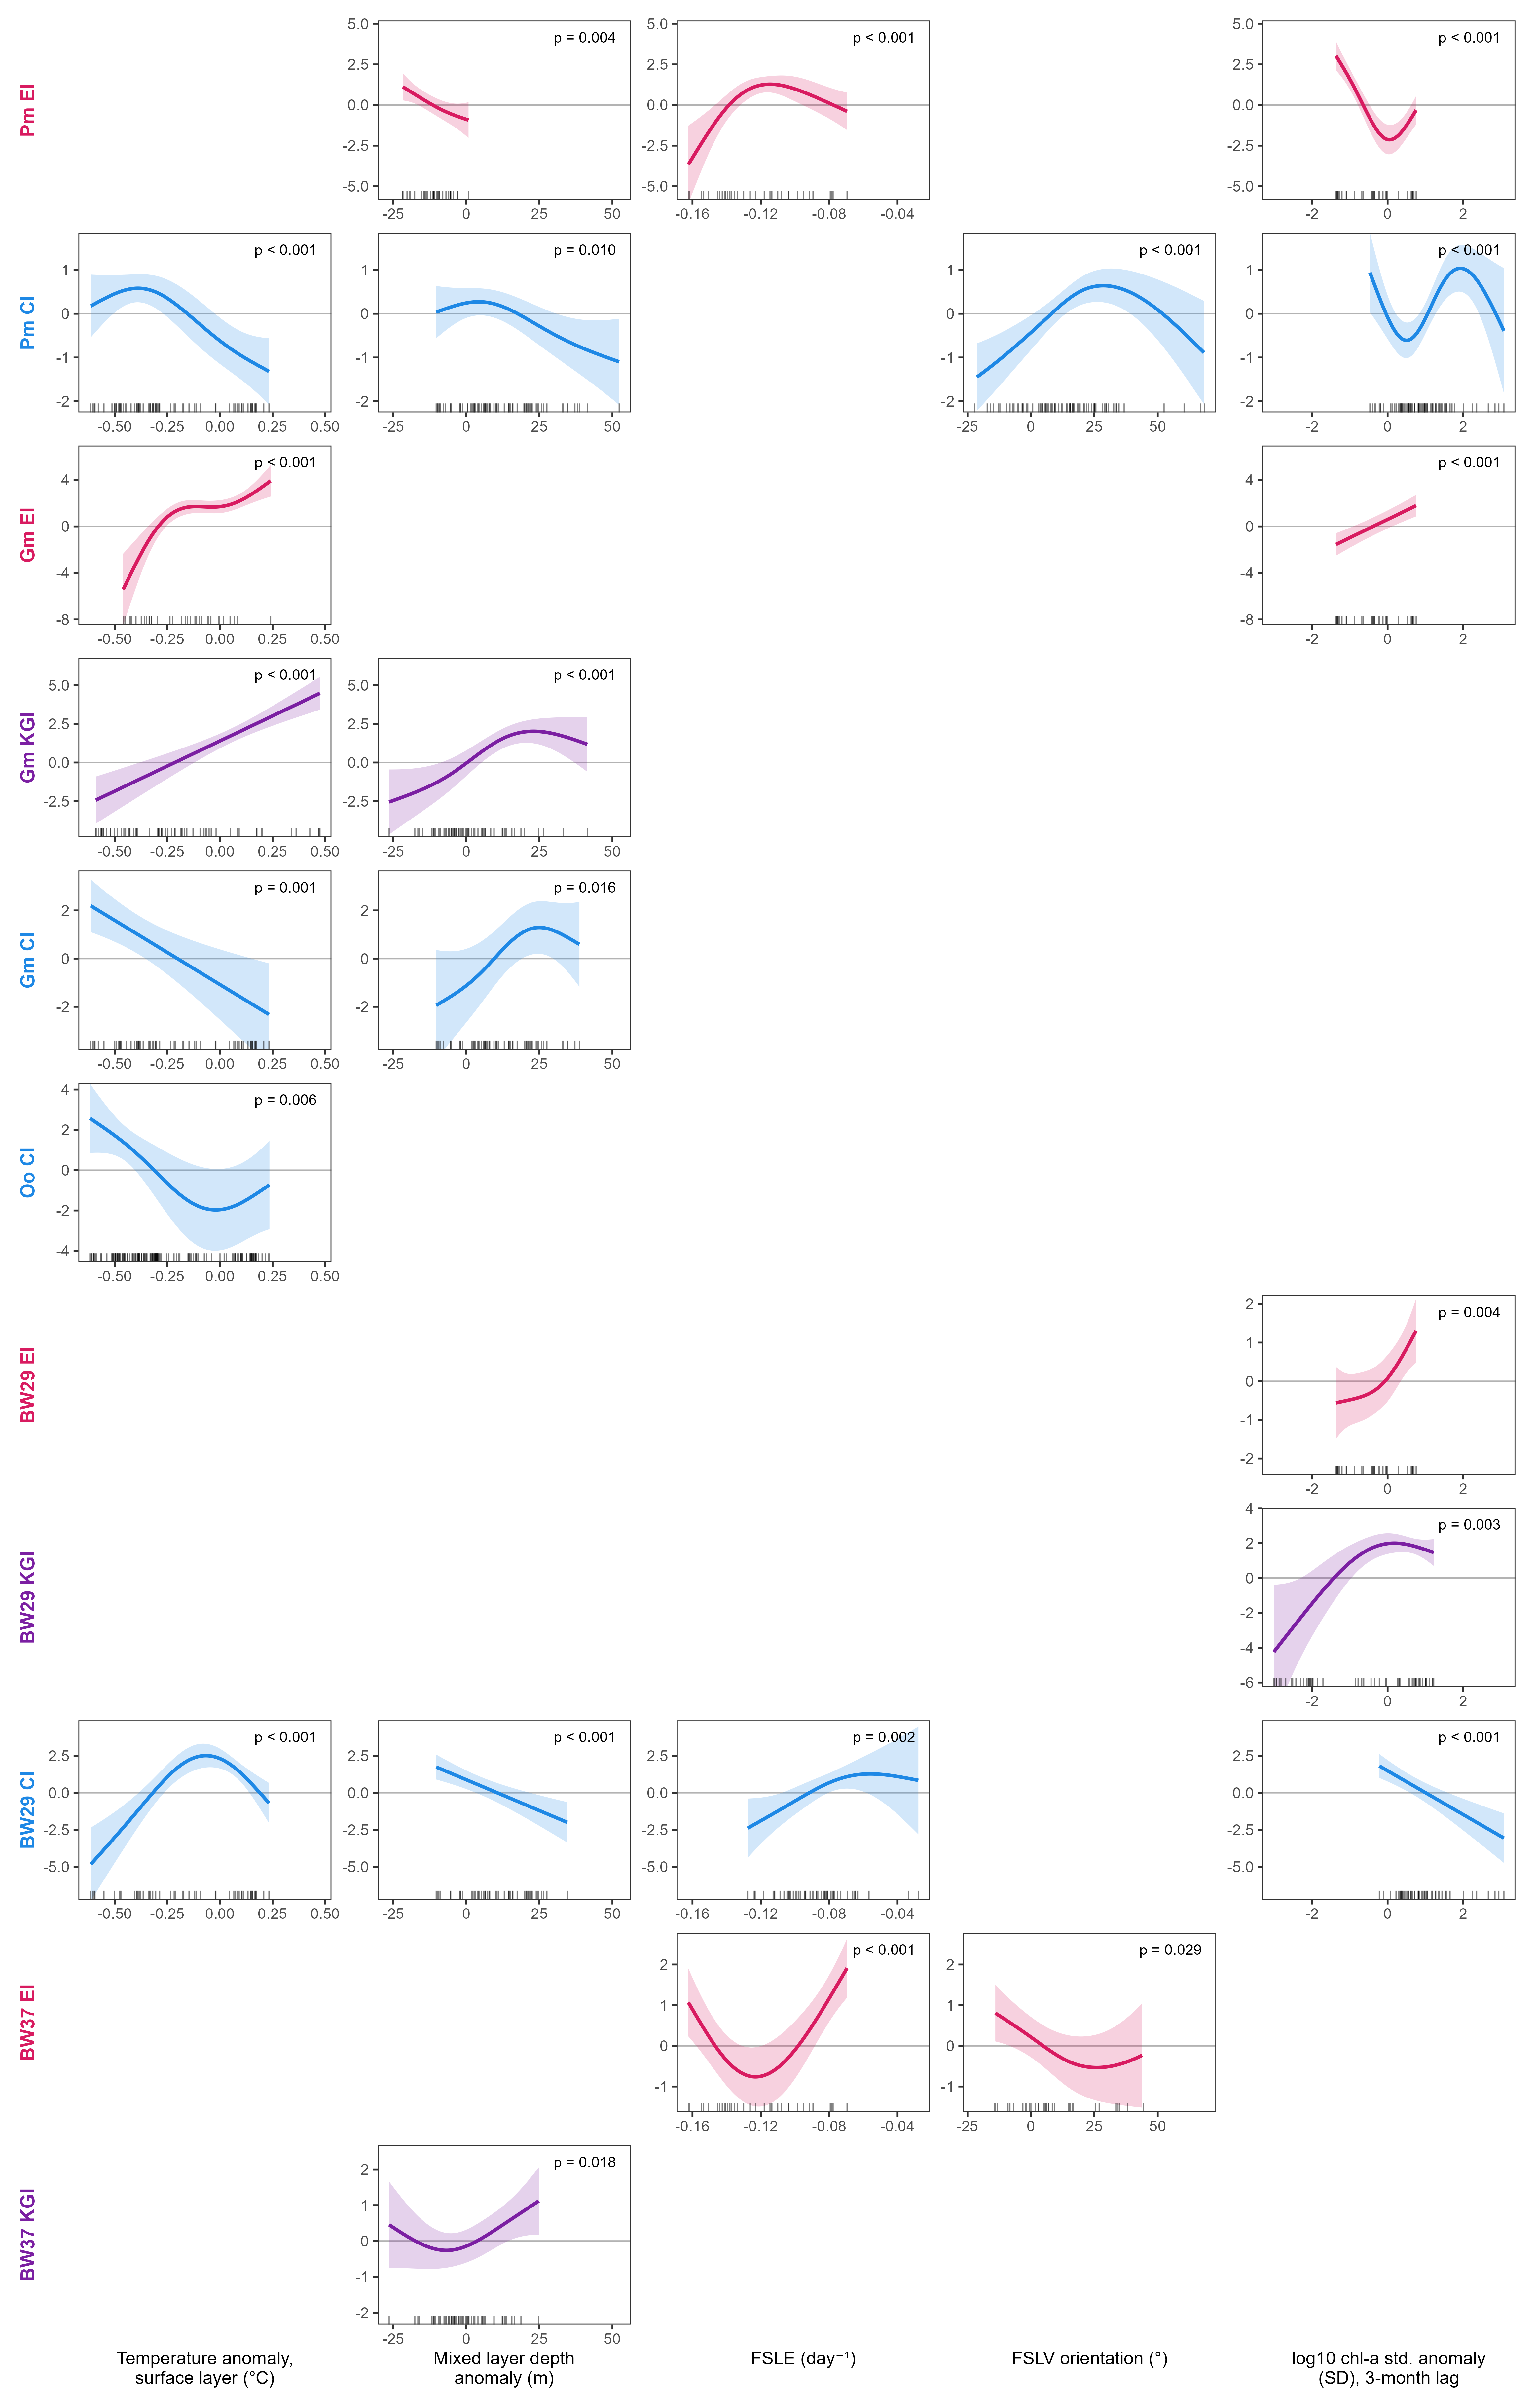
\includegraphics[width=1\linewidth,height=\textheight,keepaspectratio]{../outputs/08_results_gams/main_stage3_habitat_response_curves_grid.png}

}

\caption{\label{fig-curves}Partial effects of the significant terms in
the final habitat GAMs, by predictor and species, colored by site (EI,
KGI, CI), with 95\% confidence bands, shown over the observed range of
each predictor. \conf{legend details: line types, rugs, scale}}

\end{figure}%

\begingroup\fontsize{8}{10}\selectfont

\begin{longtable}[t]{>{\raggedright\arraybackslash}p{2.2cm}l>{\raggedright\arraybackslash}p{1.4cm}l>{\raggedright\arraybackslash}p{4cm}lll>{\raggedright\arraybackslash}p{2.6cm}}
\caption{\label{tab:habitat}Final habitat models (Tweedie GAMs) for each species and site. Predictors are anomalies from the 10-year climatology except FSLE, FSLV orientation and EKE. Term deviance explained is the decrease in deviance explained when the term is removed and the model refit, so terms need not sum to the model total. Shape describes the fitted smooth. ‡ Low-sample model (10--20 bins with detections; at most two terms). † Term not significant when residual autocorrelation was modeled with an AR(1) process, or when refit by maximum likelihood (Supplement S5). Bins were 4 days long (killer whales, 2 days).}\\
\toprule
Species & Site & Bins (det.) & Dev. (\%) & Term & edf & p & Term dev. (\%) & Shape\\
\midrule
\endfirsthead
\caption[]{Final habitat models (Tweedie GAMs) for each species and site. Predictors are anomalies from the 10-year climatology except FSLE, FSLV orientation and EKE. Term deviance explained is the decrease in deviance explained when the term is removed and the model refit, so terms need not sum to the model total. Shape describes the fitted smooth. ‡ Low-sample model (10--20 bins with detections; at most two terms). † Term not significant when residual autocorrelation was modeled with an AR(1) process, or when refit by maximum likelihood (Supplement S5). Bins were 4 days long (killer whales, 2 days). \textit{(continued)}}\\
\toprule
Species & Site & Bins (det.) & Dev. (\%) & Term & edf & p & Term dev. (\%) & Shape\\
\midrule
\endhead

\endfoot
\bottomrule
\endlastfoot
Sperm whale & EI & 34 (23) & 85.2 & FSLE & 2.30 & <0.001 & 13.1 & peaked\\
 &  &  &  & Mixed layer depth anomaly† & 1.45 & 0.004 & 8.4 & decreasing\\
 &  &  &  & Chl-a anomaly, 3-month lag† & 1.88 & <0.001 & 23.4 & U-shaped\\
Sperm whale & KGI & 89 (0) & -- & not modeled (<10 bins with detections) &  &  &  & \\
Sperm whale & CI & 76 (65) & 53.1 & FSLV orientation & 1.61 & 0.007 & 5.5 & cyclic, unimodal (peak 30°, trough -63°)\\
 &  &  &  & EKE, mid-water layer & 0.87 & 0.004 & 2.6 & decreasing\\
 &  &  &  & EKE, deep layer† & 1.58 & 0.021 & 2.5 & peaked\\
 &  &  &  & Mixed layer depth anomaly† & 1.52 & 0.029 & 4.8 & peaked\\
 &  &  &  & Temperature anomaly, surface layer & 1.79 & <0.001 & 37.2 & decreasing\\
 &  &  &  & Chl-a anomaly, 3-month lag & 1.76 & <0.001 & 10.6 & U-shaped\\
Long-finned pilot whale & EI & 34 (19)‡ & 84.8 & Temperature anomaly, surface layer & 2.78 & <0.001 & 21.1 & increasing\\
 &  &  &  & Chl-a anomaly, 3-month lag & 1.56 & <0.001 & 26.3 & increasing\\
Long-finned pilot whale & KGI & 64 (18)‡ & 31.9 & Temperature anomaly, surface layer & 1.64 & <0.001 & 31.9 & increasing\\
Long-finned pilot whale & CI & 64 (11)‡ & 48.0 & Temperature anomaly, surface layer† & 0.82 & 0.027 & 6.8 & decreasing\\
 &  &  &  & EKE, deep layer† & 1.50 & 0.010 & 15.7 & peaked\\
Killer whale & EI & 68 (3) & -- & not modeled (<10 bins with detections) &  &  &  & \\
Killer whale & KGI & 177 (3) & -- & not modeled (<10 bins with detections) &  &  &  & \\
Killer whale & CI & 151 (11)‡ & 21.1 & Chl-a anomaly, 3-month lag† & 1.57 & 0.007 & 21.1 & U-shaped\\
Southern bottlenose whale & EI & 34 (26) & 59.0 & FSLE† & 1.41 & 0.031 & 9.8 & peaked\\
 &  &  &  & Chl-a anomaly, 3-month lag† & 2.76 & <0.001 & 45.2 & complex\\
Southern bottlenose whale & KGI & 56 (20)‡ & 38.7 & Chl-a anomaly, 3-month lag & 1.93 & 0.003 & 38.7 & increasing\\
Southern bottlenose whale & CI & 52 (24) & 66.7 & FSLE & 1.44 & 0.003 & 11.8 & peaked\\
 &  &  &  & Chl-a anomaly, 3-month lag & 0.96 & <0.001 & 30.2 & decreasing\\
 &  &  &  & Mixed layer depth anomaly & 0.90 & 0.003 & 6.9 & decreasing\\
 &  &  &  & Temperature anomaly, surface layer & 1.87 & <0.001 & 27.0 & peaked\\
BW37 beaked whale & EI & 34 (17)‡ & 47.8 & FSLE & 1.84 & <0.001 & 34.7 & U-shaped\\
 &  &  &  & FSLV orientation & 1.35 & 0.029 & 11.5 & cyclic, unimodal (peak -66°, trough 26°)\\
BW37 beaked whale & KGI & 56 (27) & 42.5 & Mixed layer depth anomaly† & 1.40 & 0.018 & 8.4 & U-shaped\\
 &  &  &  & Temperature anomaly, deep layer & 1.80 & <0.001 & 34.1 & peaked\\
BW37 beaked whale & CI & 52 (7) & -- & not modeled (<10 bins with detections) &  &  &  & \\*
\end{longtable}
\endgroup{}

\section{Discussion}\label{discussion}

\ins{Discussion to be written. Points noted so far: residual autocorrelation remained in 2 of 11 habitat models (Ljung--Box p ≤ 0.05; long-finned pilot whales at KGI and southern bottlenose whales at CI), and AR(1) retained 14 of 24 testable terms; lagged chlorophyll-a effects were not robust; EKE box-averaging caveat; qualitative description of the rare species--site combinations.}

\clearpage

\section*{Supplementary material}\label{supplementary-material}
\addcontentsline{toc}{section}{Supplementary material}

\setcounter{figure}{0}
\setcounter{table}{0}
\renewcommand{\thefigure}{S\arabic{figure}}
\renewcommand{\thetable}{S\arabic{table}}

\subsection*{S1. Depth-layer
boundaries}\label{s1.-depth-layer-boundaries}
\addcontentsline{toc}{subsection}{S1. Depth-layer boundaries}

The layer boundaries were derived from the reanalysis at all three sites
using two independent lines of evidence (Figure~\ref{fig-layers}).
First, depths were grouped by how similarly their daily
temperature--salinity anomalies varied over the 10-year record, using
depth-constrained clustering (CONISS; Grimm 1987). Second, we identified
water-mass features in the 10-year mean profiles: the deepest winter
mixed layer, the Winter Water temperature minimum, the main pycnocline,
and the warm-water core of Circumpolar Deep Water. The surface-layer
base (100 m) lies below the deepest winter mixed layer and the Winter
Water minimum (51--92 m) and coincides with the coherence breaks at EI
and KGI (102--118 m). The mid-water layer contains the warm Circumpolar
Deep Water core (temperature maximum at 266--454 m), and its base (500
m) lies near the coherence breaks below that core at EI and CI (462--502
m; 692 m at KGI). The deep layer was capped at 1000 m because, below
\textasciitilde1060 m, less than half of the KGI and CI boxes contains
water.

\begin{figure}[htbp]

\centering{

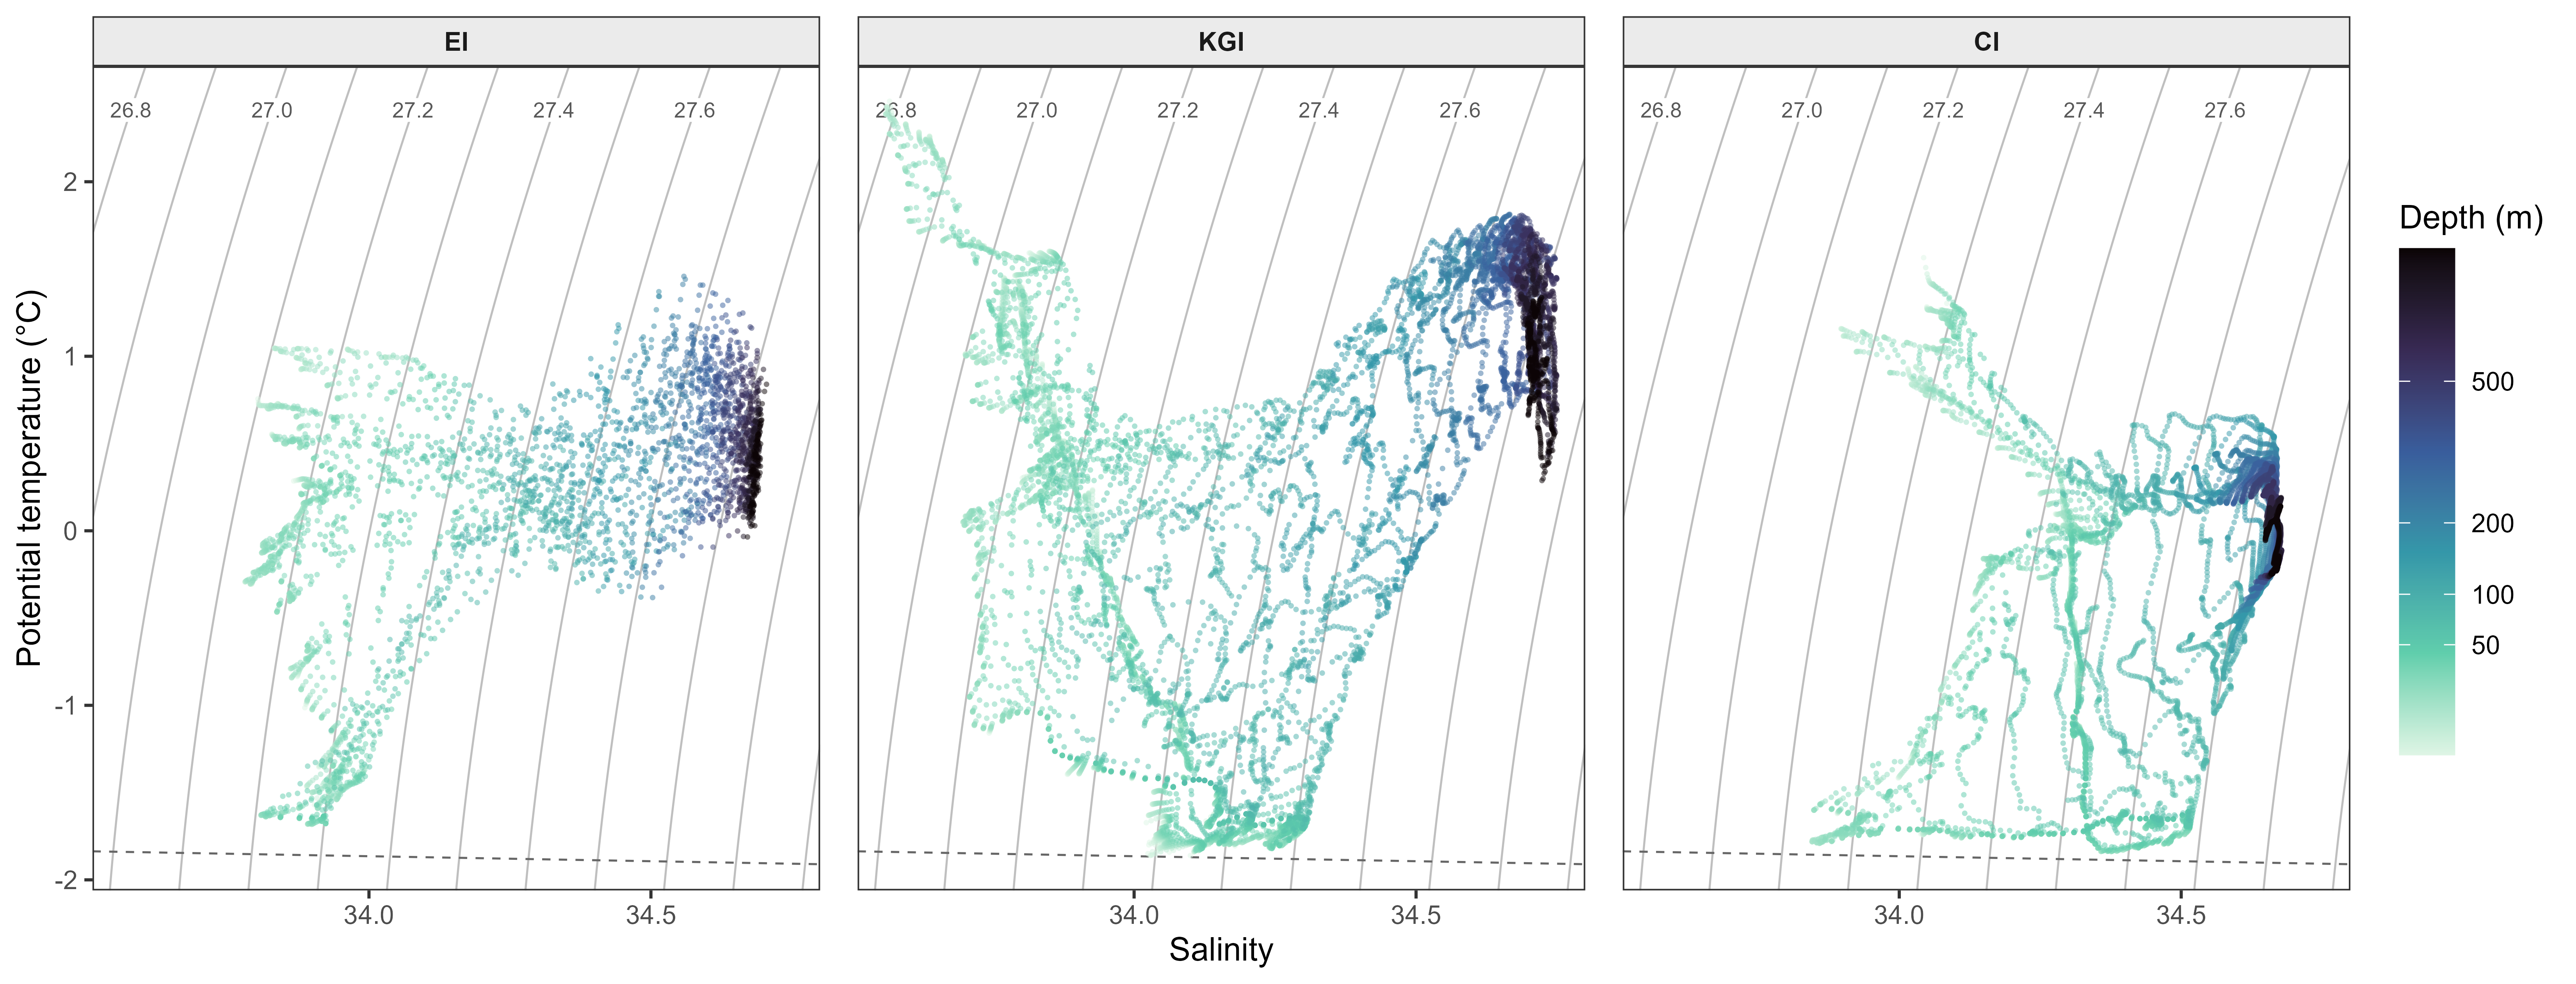
\includegraphics[width=1\linewidth,height=\textheight,keepaspectratio]{../outputs/02_deep_oceanography/ts_diagram.png}

}

\caption{\label{fig-ts}Temperature--salinity diagrams for EI, KGI, and
CI over each site's recording period. Each point is a daily box-mean
(±20 km) value at one model level (0.5--1000 m) from the Copernicus
Marine Service global physics reanalysis, colored by depth (square-root
scale). Grey contours show potential density anomaly (\(\sigma_\theta\),
kg m\(^{-3}\); labelled every 0.2 kg m\(^{-3}\)), and the dashed line
shows the surface freezing temperature.}

\end{figure}%

\begin{figure}[htbp]

\centering{

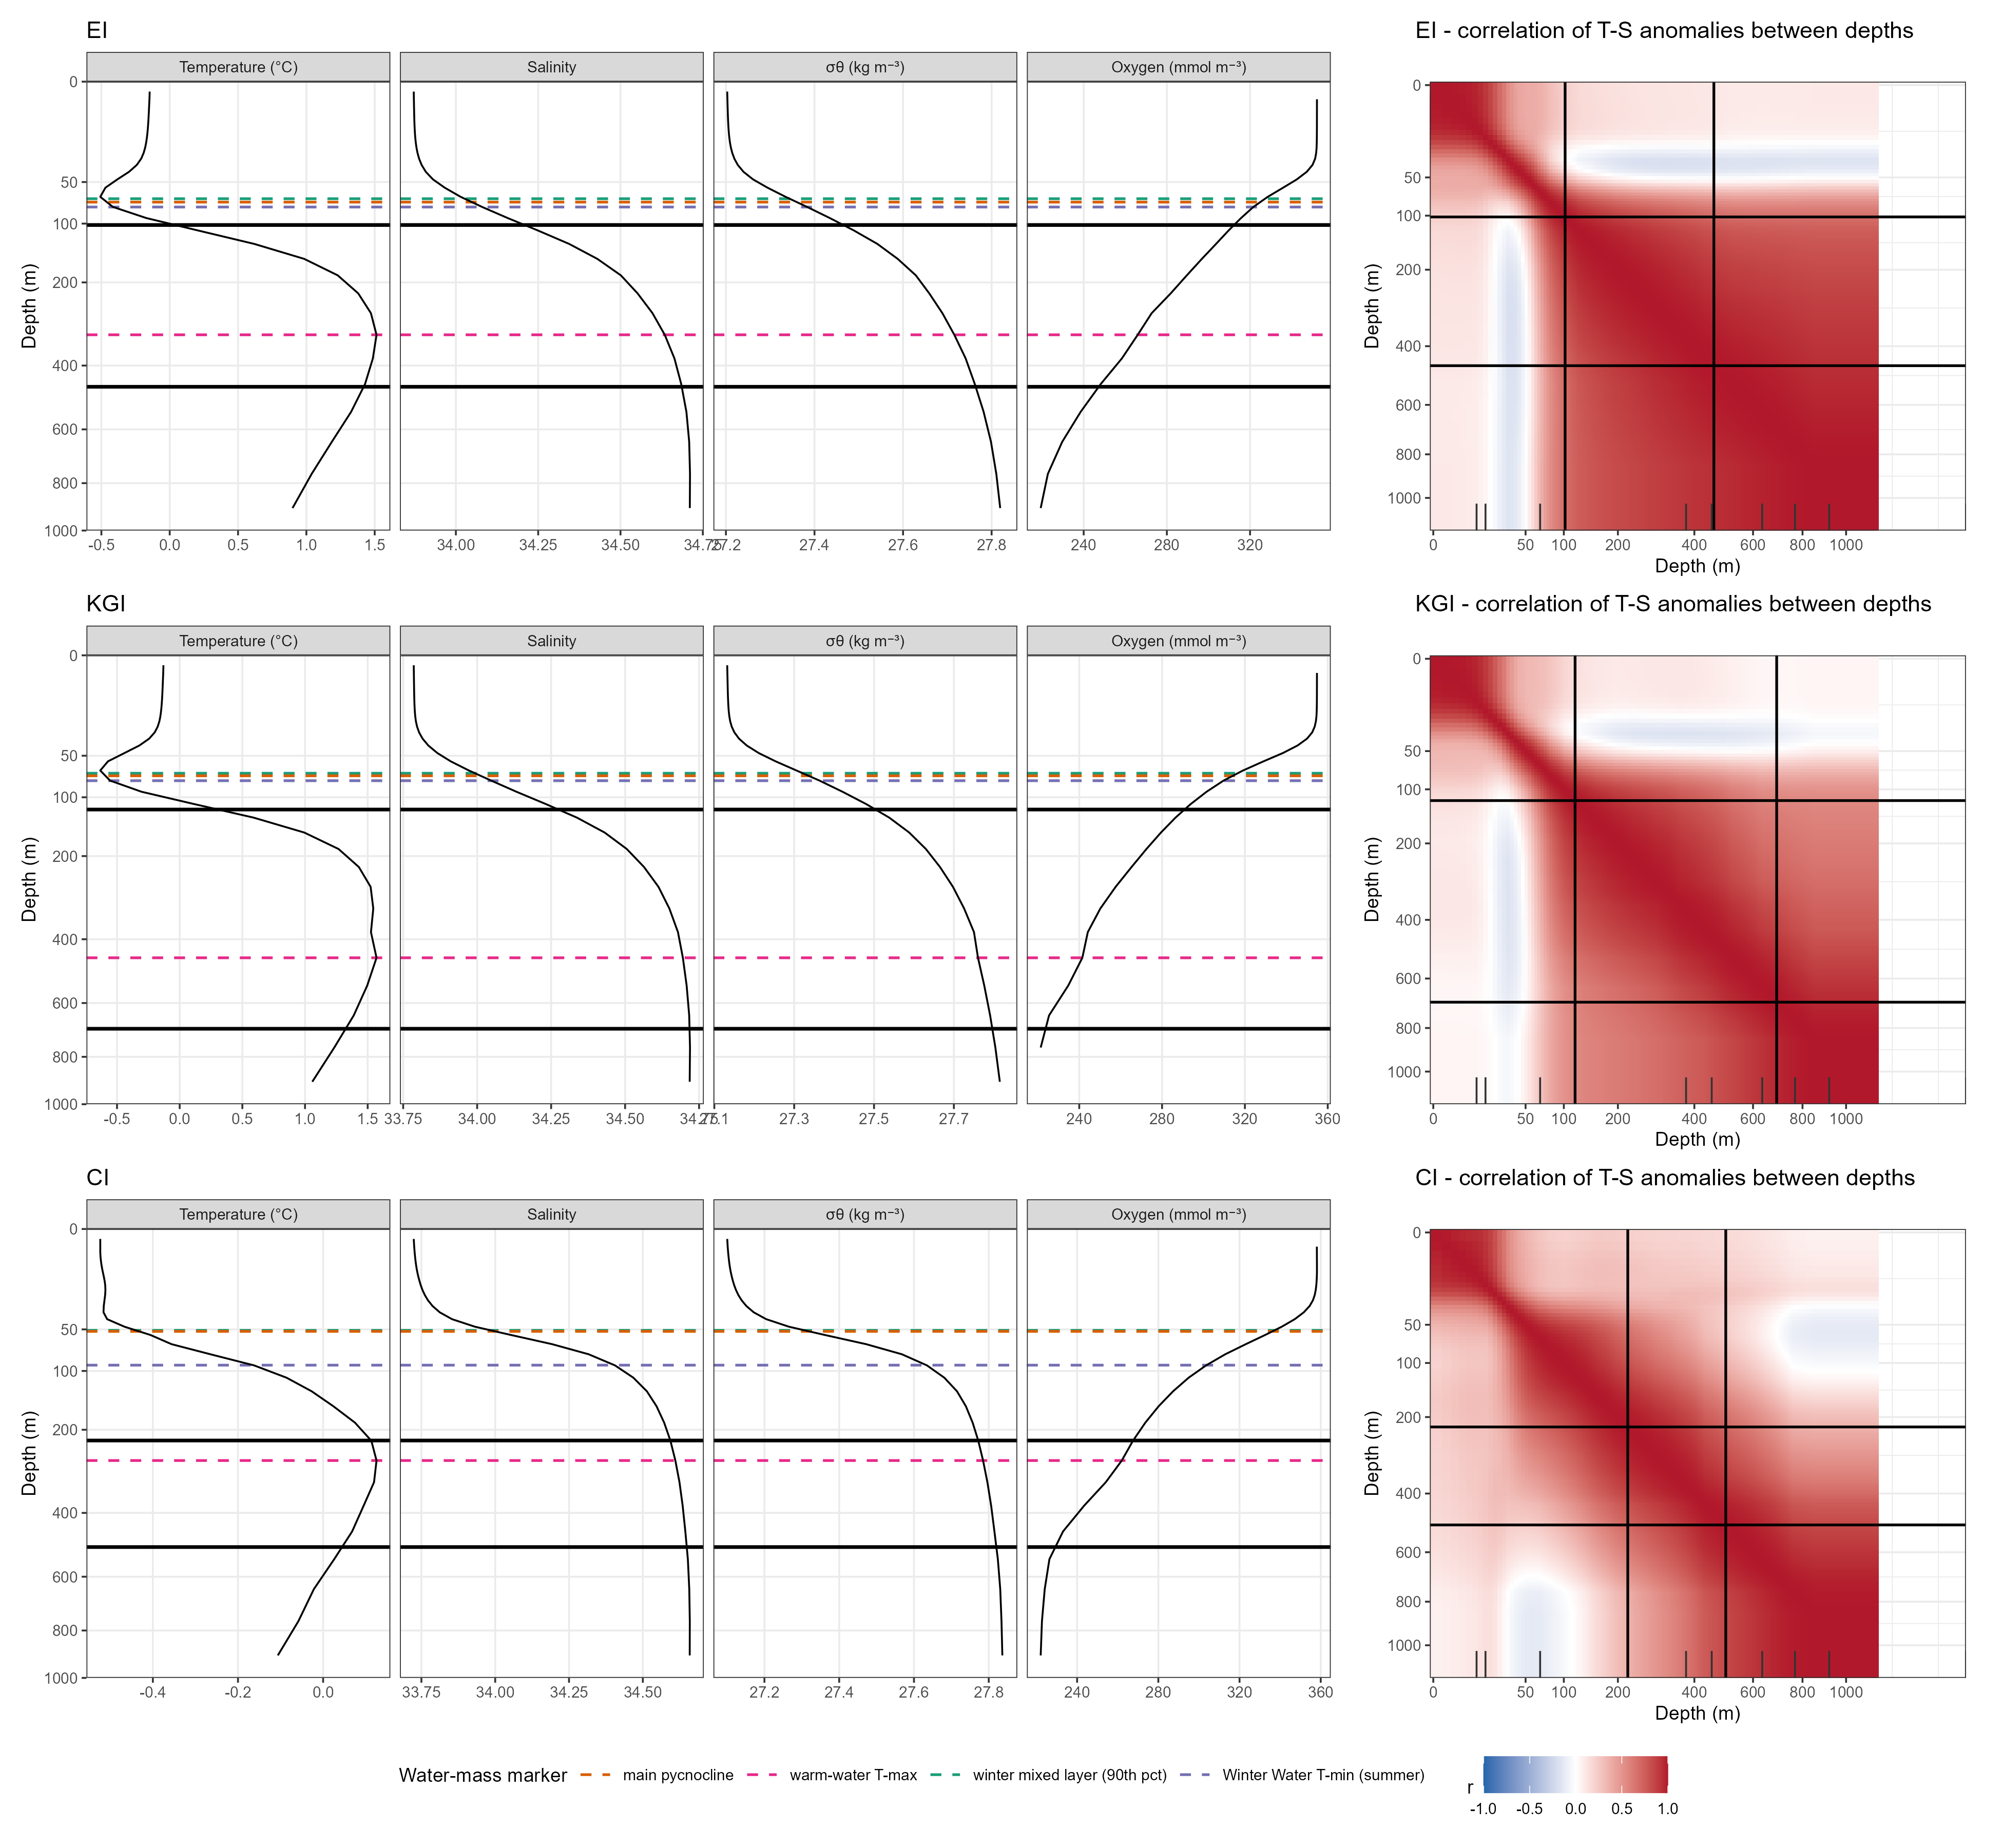
\includegraphics[width=1\linewidth,height=\textheight,keepaspectratio]{../outputs/02_deep_oceanography/layer_boundaries.png}

}

\caption{\label{fig-layers}Evidence for the depth-layer boundaries at
EI, KGI and CI. Left: 10-year mean profiles of potential temperature,
salinity, potential density anomaly (\(\sigma_\theta\)) and dissolved
oxygen, with water-mass markers (dashed): deepest winter mixed layer
(90th percentile of daily mixed layer depth), Winter Water temperature
minimum (December--March mean profile), main pycnocline (maximum density
gradient below the winter mixed layer), and the warm-water temperature
maximum. Solid lines: boundaries of the three most coherent depth
groups. Right: correlation between depths of daily temperature--salinity
anomalies (seasonal cycle removed) over the 10-year record, with the
coherence boundaries (CONISS clustering) and species depths (ticks). The
adopted layers are 0--100, 100--500 and 500--1000 m.}

\end{figure}%

\subsection*{S2. Sea-ice cutoffs and duty
cycling}\label{s2.-sea-ice-cutoffs-and-duty-cycling}
\addcontentsline{toc}{subsection}{S2. Sea-ice cutoffs and duty cycling}

\begin{table}[!h]
\centering
\caption{\label{tab:icecut}Sea-ice cutoffs for the habitat models and the number of time bins removed at each site. The cutoff is the highest bin-mean sea-ice concentration at which the species was detected at any site. Bin length was 4 days for all species except killer whales (2 days).}
\centering
\fontsize{9}{11}\selectfont
\begin{tabular}[t]{lllll}
\toprule
Species & Cutoff (\% ice) & EI removed/total & KGI removed/total & CI removed/total\\
\midrule
Sperm whale & 84.5 & 0/34 & -- (not detected) & 0/76\\
Long-finned pilot whale & 33.4 & 0/34 & 25/89 & 12/76\\
Killer whale & 88.9 & 0/68 & 0/177 & 1/152\\
Southern bottlenose whale & 12.6 & 0/34 & 33/89 & 24/76\\
BW37 beaked whale & 12.6 & 0/34 & 33/89 & 24/76\\
\bottomrule
\end{tabular}
\end{table}

\textbackslash begin\{table\}{[}!h{]} \centering
\textbackslash caption\{\label{tab:duty}Duty-cycle subsampling of
continuous CI recordings (mean \% retained, range across 100 phase
offsets). BW58 was not detected at CI and could not be evaluated.\}
\centering \fontsize{9}{11}\selectfont

\begin{tabular}[t]{lllll}
\toprule
Species & Duty cycle & Events & 5-min bins & Presence days\\
\midrule
Sperm whale & EI (5 of 6 min) & 87.1 (84.6–90.1) & 94.0 (92.7–95.4) & 93.5 (90.1–96.7)\\
Sperm whale & KGI (10 of 13.33 min) & 79.1 (75.9–84.4) & 89.6 (88.3–91.5) & 89.6 (84.1–94.0)\\
Long-finned pilot whale & EI (5 of 6 min) & 100.0 & 99.1 (97.8–100.0) & 100.0\\
Long-finned pilot whale & KGI (10 of 13.33 min) & 95.0 (86.8–100.0) & 95.7 (90.5–99.3) & 97.3 (86.7–100.0)\\
Killer whale & EI (5 of 6 min) & 98.2 (87.0–100.0) & 99.3 (97.8–100.0) & 100.0\\
Killer whale & KGI (10 of 13.33 min) & 94.3 (82.6–100.0) & 96.7 (94.0–98.5) & 100.0\\
Southern bottlenose whale & EI (5 of 6 min) & 100.0 & 98.4 (97.5–100.0) & 100.0\\
Southern bottlenose whale & KGI (10 of 13.33 min) & 90.0 (87.2–92.4) & 90.6 (88.3–92.6) & 98.5 (94.1–100.0)\\
BW37 beaked whale & EI (5 of 6 min) & 100.0 & 99.3 (96.3–100.0) & 100.0\\
BW37 beaked whale & KGI (10 of 13.33 min) & 92.3 (83.3–100.0) & 92.5 (81.5–100.0) & 96.5 (90.9–100.0)\\
\bottomrule
\end{tabular}

\textbackslash end\{table\}

\begin{figure}[htbp]

\centering{

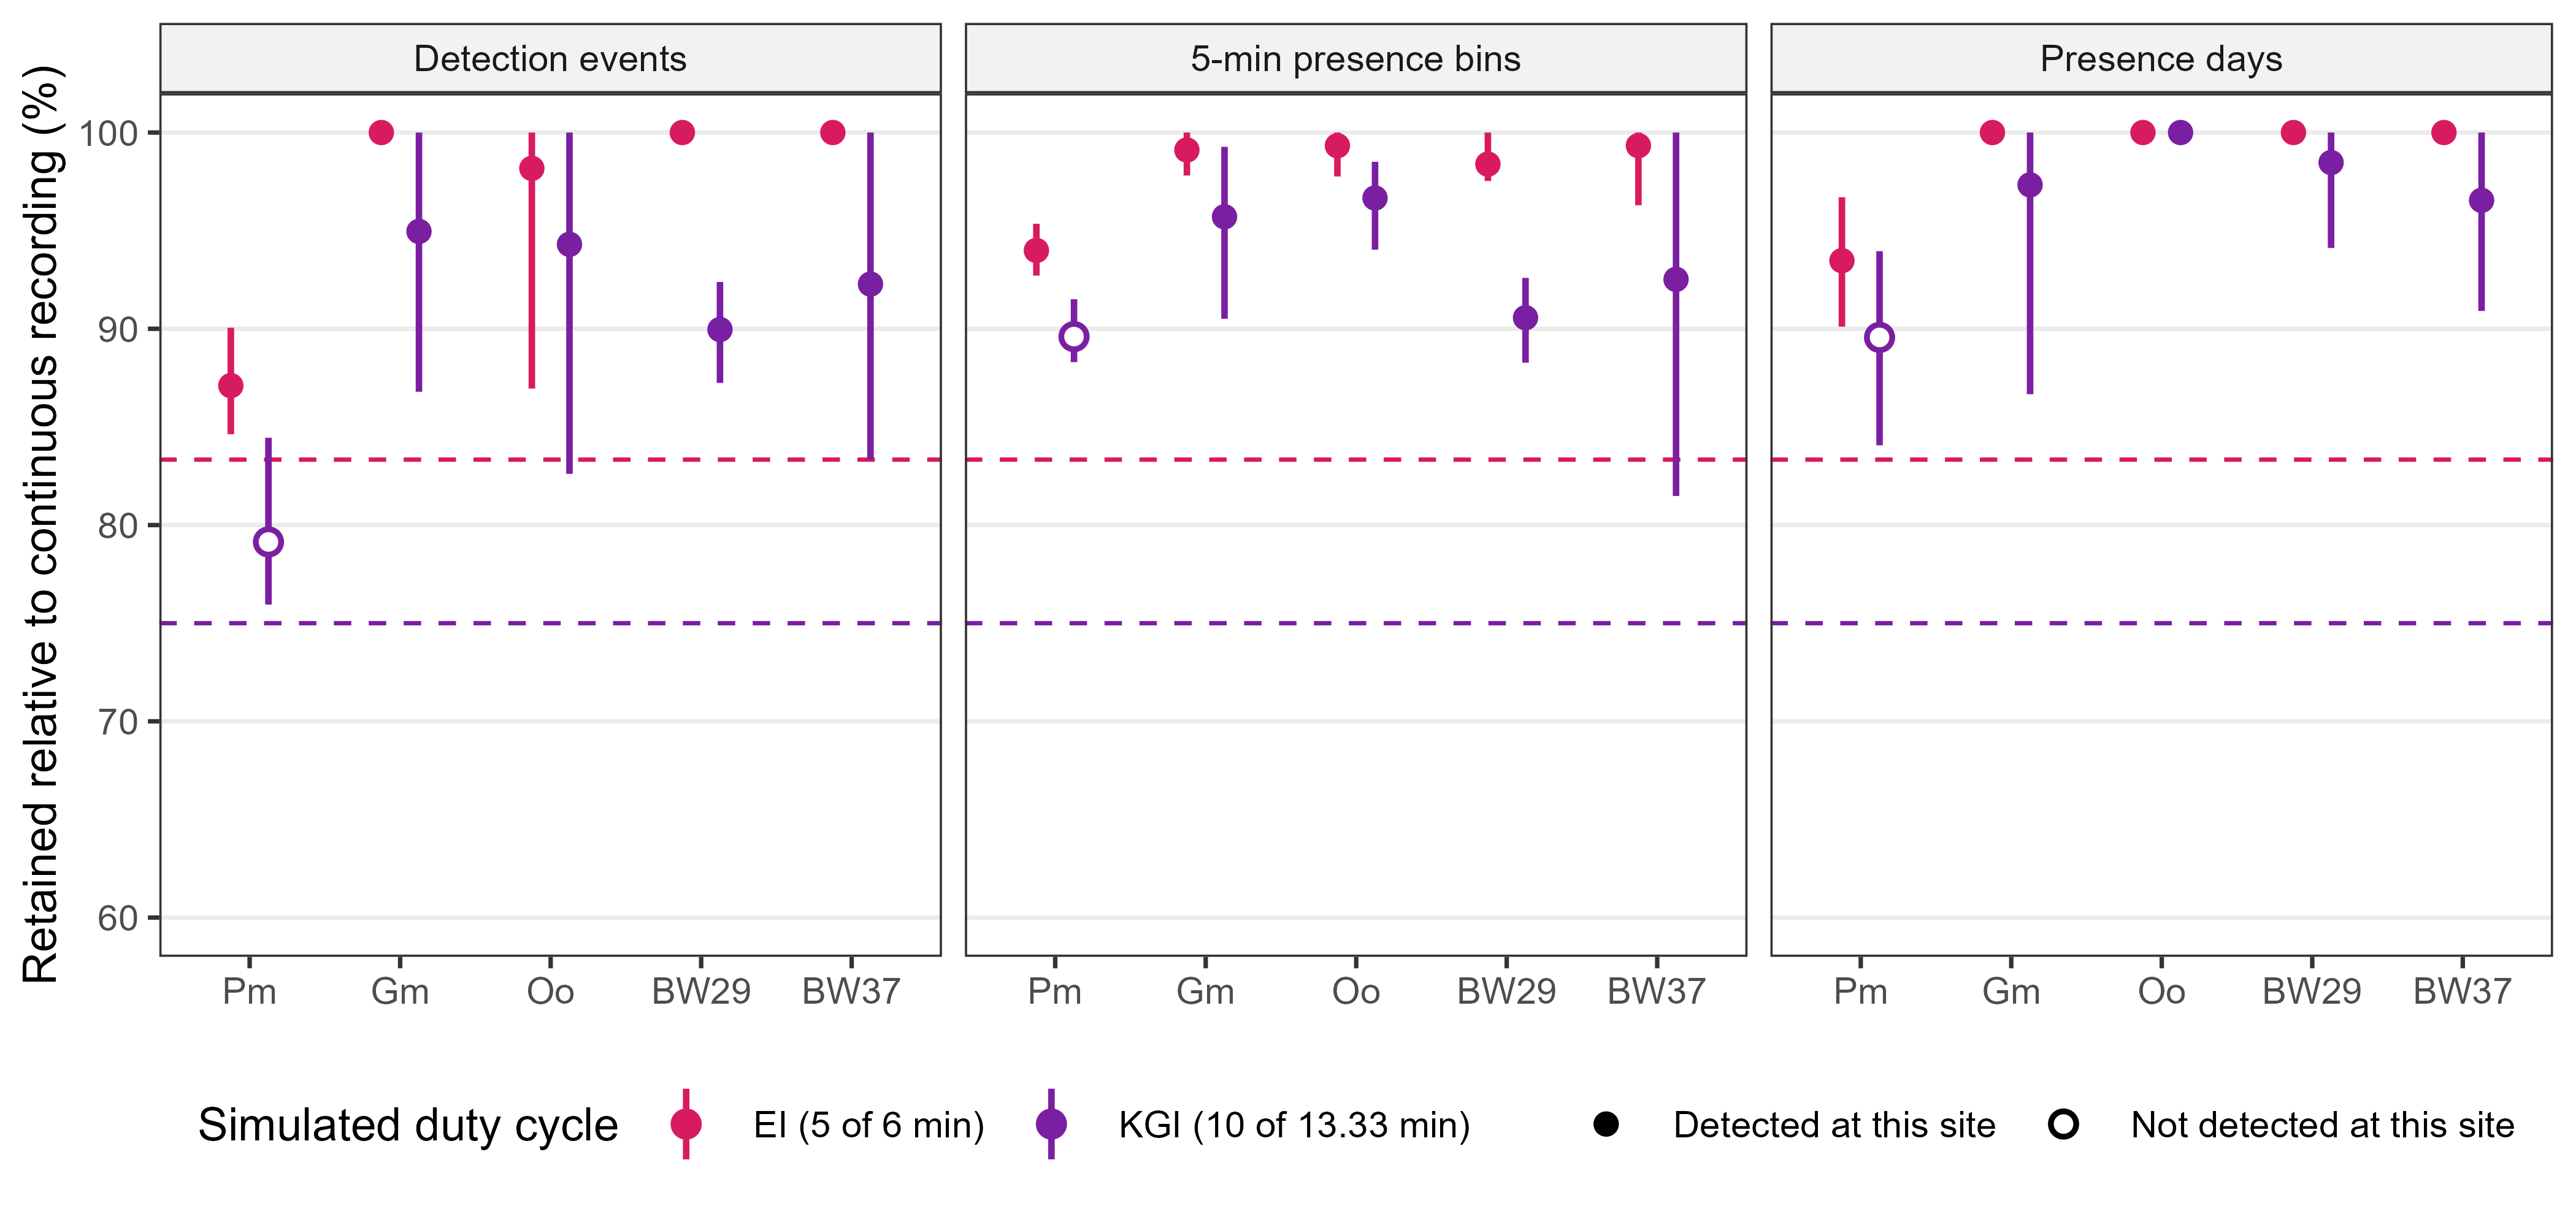
\includegraphics[width=0.85\linewidth,height=\textheight,keepaspectratio]{../outputs/04_acoustic_detection/duty_cycle_simulation.png}

}

\caption{\label{fig-duty}Effect of duty cycling on odontocete
detections, estimated by subsampling the continuous recordings at
Clarence Island (CI) to the duty cycles used at Elephant Island (EI; 5
min on every 6 min) and King George Island (KGI; 10 min on every 13.33
min) at 100 random phase offsets. Panels show the percentage of
detection events, positive 5-min bins, and presence days retained
relative to continuous recording. Points show the mean and bars the
range across phase offsets. Dashed horizontal lines mark the proportion
of time recorded under each duty cycle (83.3\% for EI, 75.0\% for KGI).
Open symbols mark species not detected at the site whose duty cycle was
simulated (sperm whale at KGI). BW58 is not shown because it was not
detected at CI. Pm, sperm whale; Gm, long-finned pilot whale; Oo, killer
whale; BW29, southern bottlenose whale; BW37, BW37 beaked whale.}

\end{figure}%

\subsection*{S3. Ocean model comparison and
validation}\label{s3.-ocean-model-comparison-and-validation}
\addcontentsline{toc}{subsection}{S3. Ocean model comparison and
validation}

\begin{figure}[htbp]

\centering{

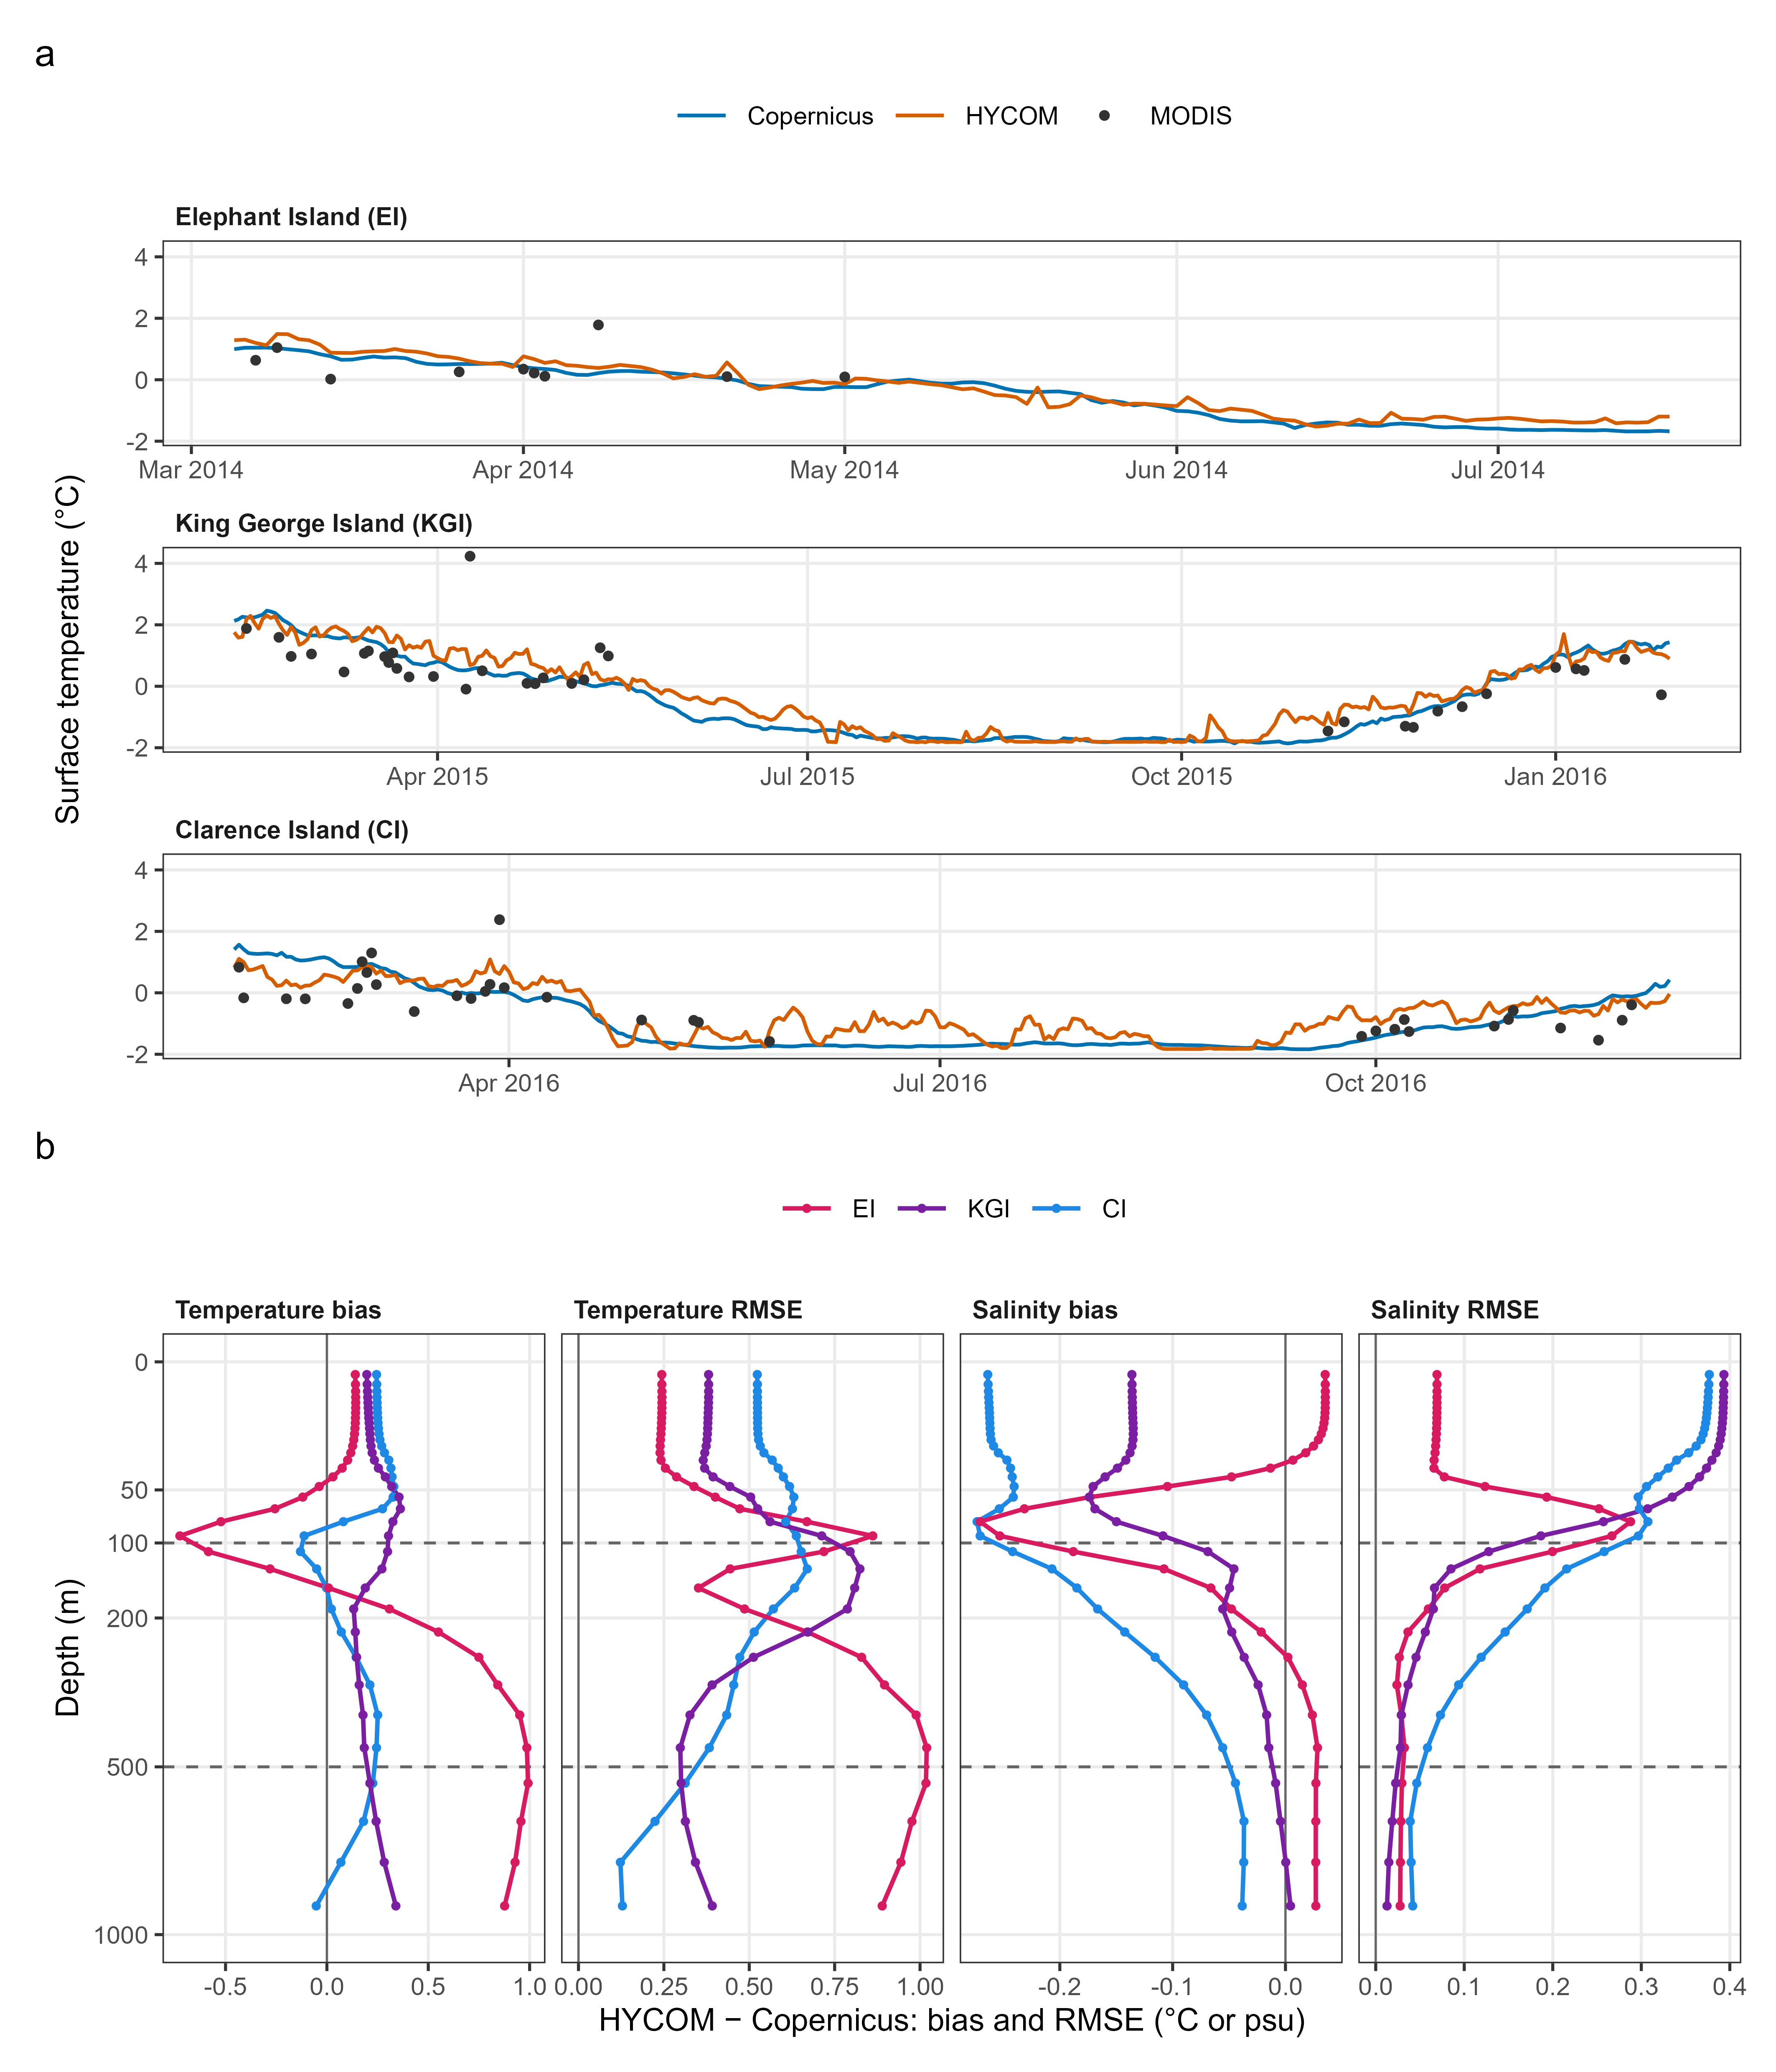
\includegraphics[width=1\linewidth,height=\textheight,keepaspectratio]{../outputs/05b_hycom_comparison/FigS3_hycom_copernicus.png}

}

\caption{\label{fig-hycom}Comparison of the Copernicus reanalysis with
HYCOM and MODIS over each site's recording period (±20 km box). (a)
Daily surface temperature from Copernicus (blue), HYCOM (orange) and
Aqua MODIS (points; days with ≥ 20\% valid pixels) at EI, KGI and CI.
(b) Bias (HYCOM − Copernicus) and root-mean-square error of daily
temperature and salinity at every Copernicus model level to 1000 m, by
site; dashed lines mark the layer boundaries (100 and 500 m).}

\end{figure}%

\begin{figure}[htbp]

\centering{

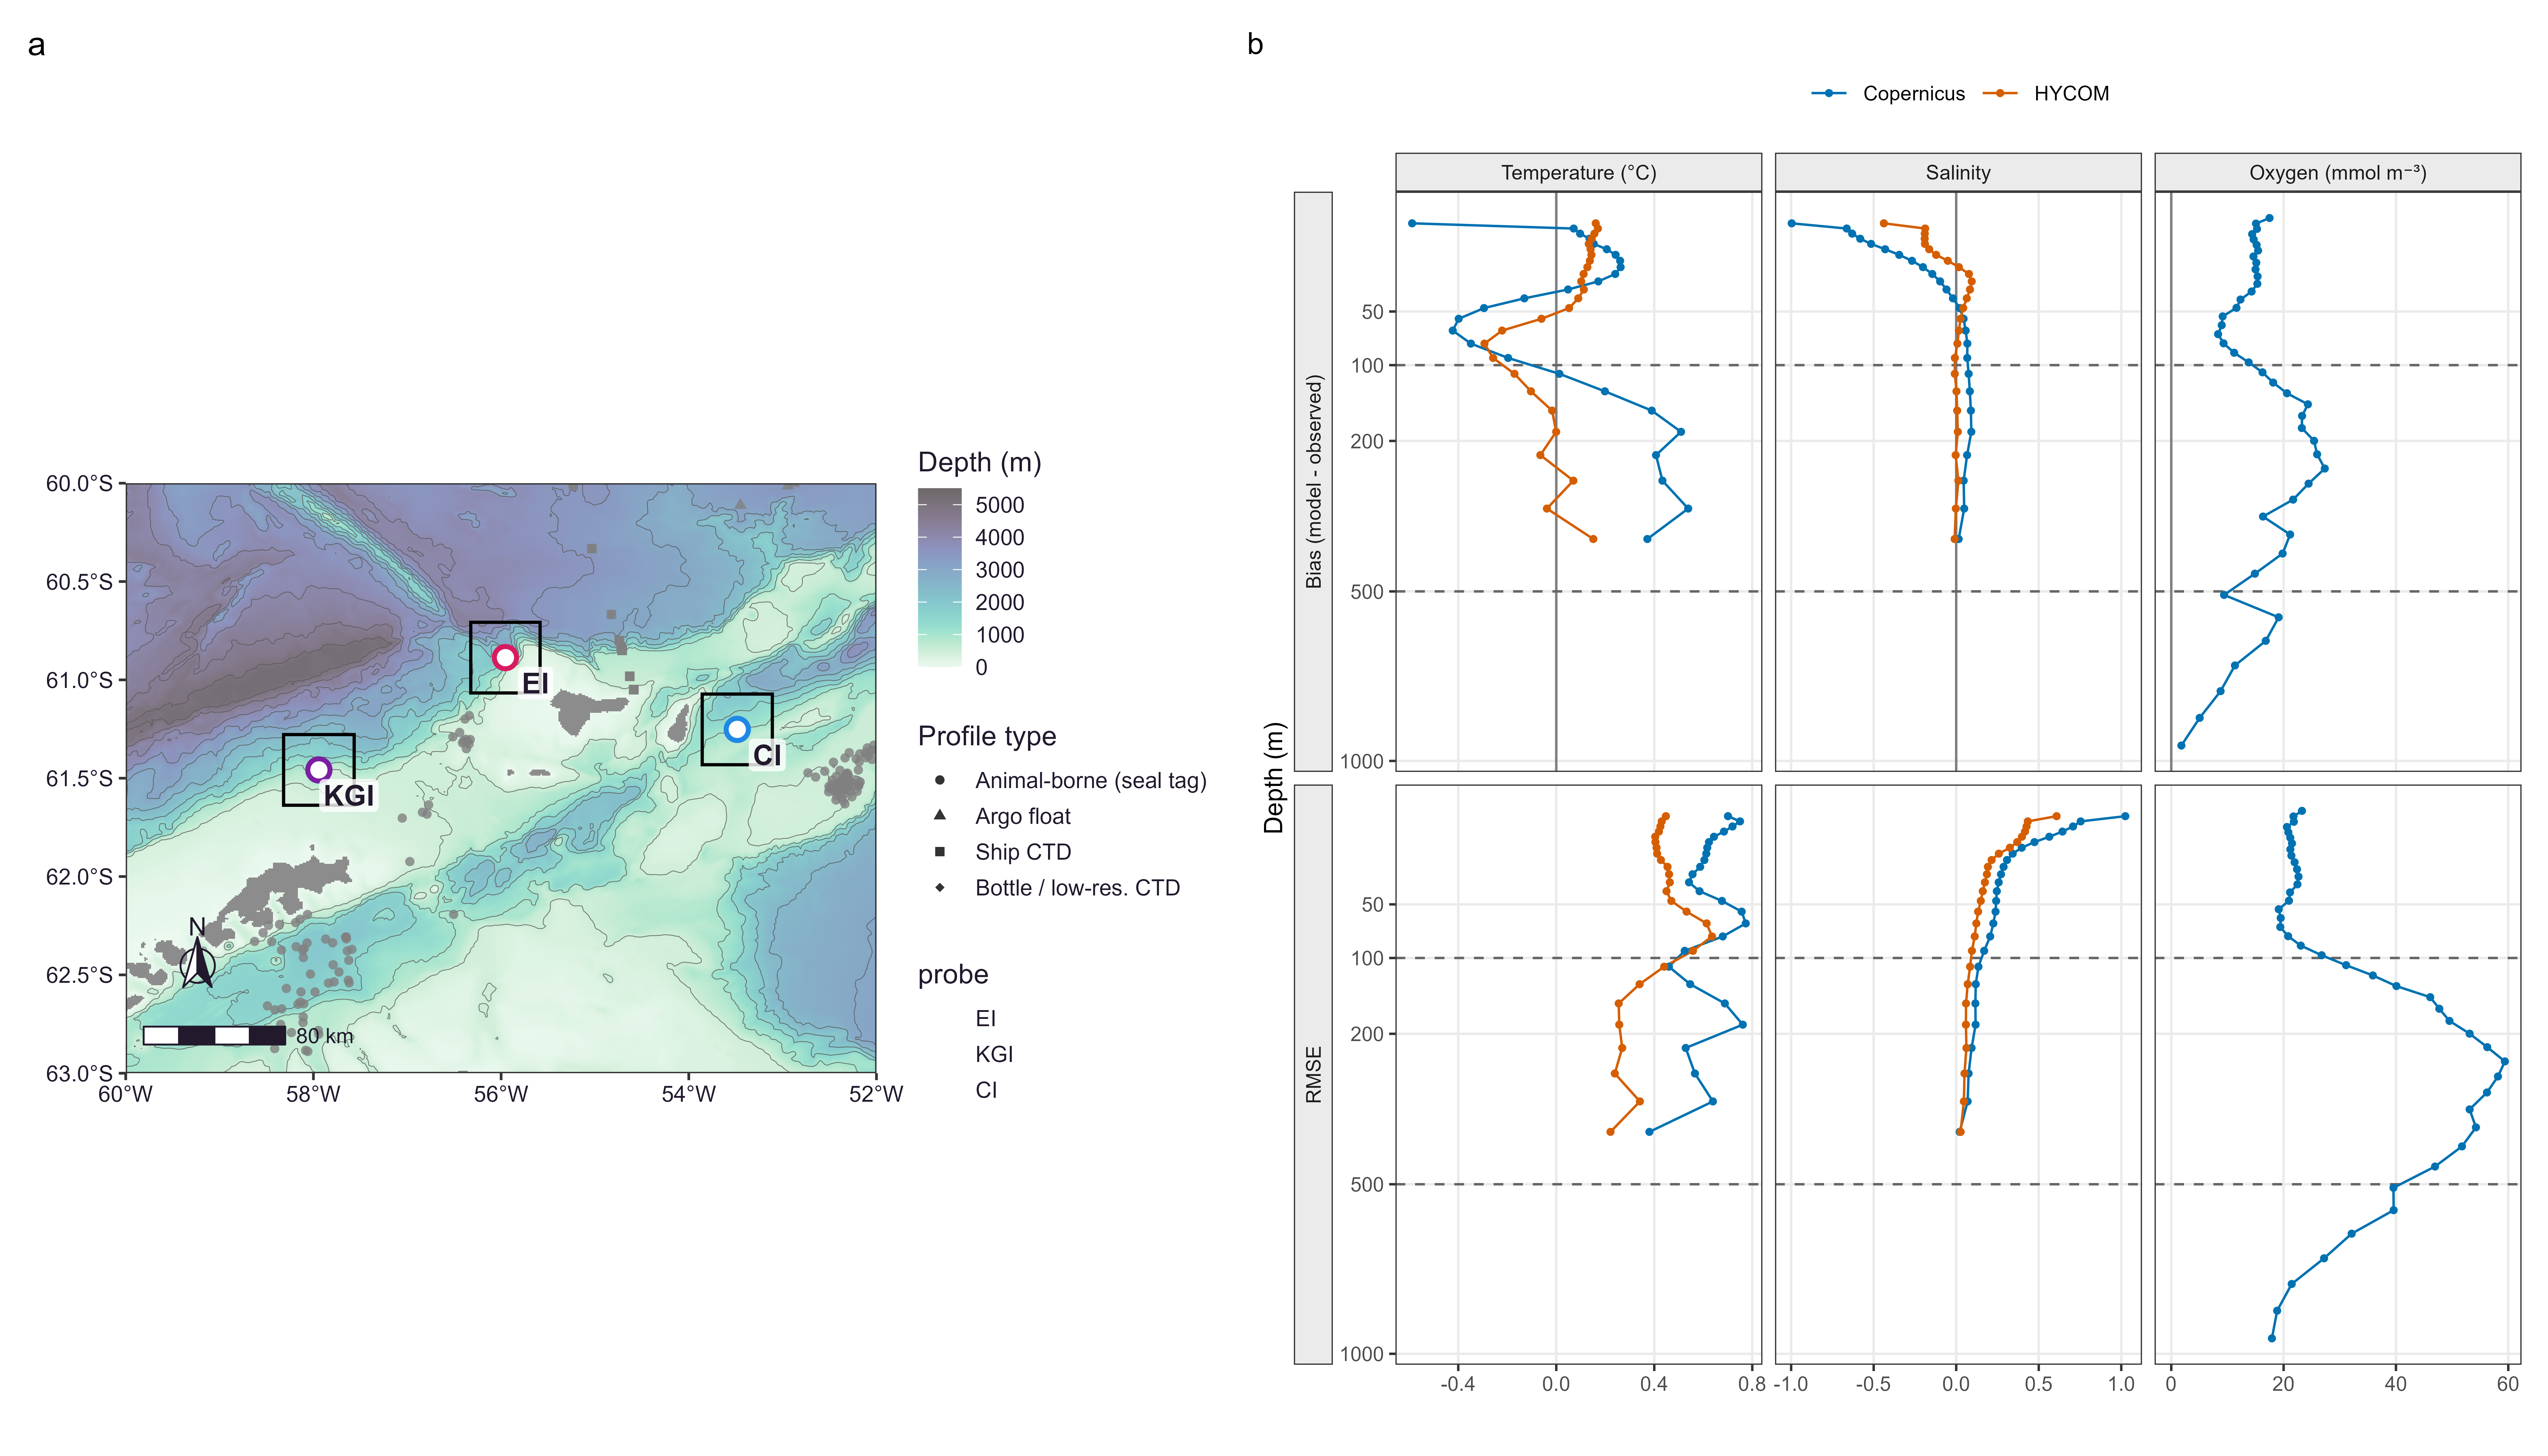
\includegraphics[width=1\linewidth,height=\textheight,keepaspectratio]{../outputs/05b_hycom_comparison/FigS4_insitu_validation.png}

}

\caption{\label{fig-insitu}Validation of the Copernicus and HYCOM models
against in-situ profiles from the World Ocean Database, 2014--2016. (a)
Locations of the 915 profiles by instrument type, with the ±20 km boxes
around the recording sites; bathymetry from GMRT. (b) Bias (model −
observed, top) and root-mean-square error (bottom) of temperature,
salinity and dissolved oxygen (Copernicus only) at each model level,
computed on the same profiles and levels for both models (levels with ≥
10 matched profiles). Dashed lines mark the layer boundaries (100 and
500 m).}

\end{figure}%

\subsection*{S4. Sea-ice models}\label{s4.-sea-ice-models}
\addcontentsline{toc}{subsection}{S4. Sea-ice models}

\begin{table}[!h]
\centering
\caption{\label{tab:seaice}Sea-ice models (presence ~ s(sea-ice concentration)) for each species and site, using all bins. Robust to AR(1): whether the effect remained significant when residual autocorrelation was modeled with an AR(1) process (significant effects only). ‡ Low-sample model (10--20 bins with detections).}
\centering
\fontsize{8}{10}\selectfont
\begin{tabular}[t]{llllllll}
\toprule
Species & Site & Bins (det.) & edf & p & Dev. (\%) & Shape & Robust to AR(1)\\
\midrule
Sperm whale & EI & 34 (23) & 0.73 & 0.064 & 6.5 & not significant & \\
Sperm whale & KGI & 89 (0) & -- & -- & -- & not modeled & \\
Sperm whale & CI & 76 (65) & 1.60 & 0.002 & 11.7 & peaked & no\\
Long-finned pilot whale & EI & 34 (19)‡ & 2.21 & <0.001 & 34.7 & peaked & no\\
Long-finned pilot whale & KGI & 89 (18)‡ & 1.67 & 0.183 & 27.9 & not significant & \\
Long-finned pilot whale & CI & 76 (11)‡ & 0.60 & 0.208 & 3.8 & not significant & \\
Killer whale & EI & 68 (3) & -- & -- & -- & not modeled & \\
Killer whale & KGI & 177 (3) & -- & -- & -- & not modeled & \\
Killer whale & CI & 152 (11)‡ & 1.66 & <0.001 & 28.5 & peaked & no\\
Southern bottlenose whale & EI & 34 (26) & 0.09 & 0.292 & 0.5 & not significant & \\
Southern bottlenose whale & KGI & 89 (20)‡ & 0.85 & 0.041 & 32.9 & decreasing & yes\\
Southern bottlenose whale & CI & 76 (24) & 0.92 & <0.001 & 56.1 & decreasing & yes\\
BW37 beaked whale & EI & 34 (17)‡ & 0.83 & 0.201 & 5.3 & not significant & \\
BW37 beaked whale & KGI & 89 (27) & 0.90 & 0.009 & 35.5 & decreasing & yes\\
BW37 beaked whale & CI & 76 (7) & -- & -- & -- & not modeled & \\
\bottomrule
\end{tabular}
\end{table}

\begin{figure}[htbp]

\centering{

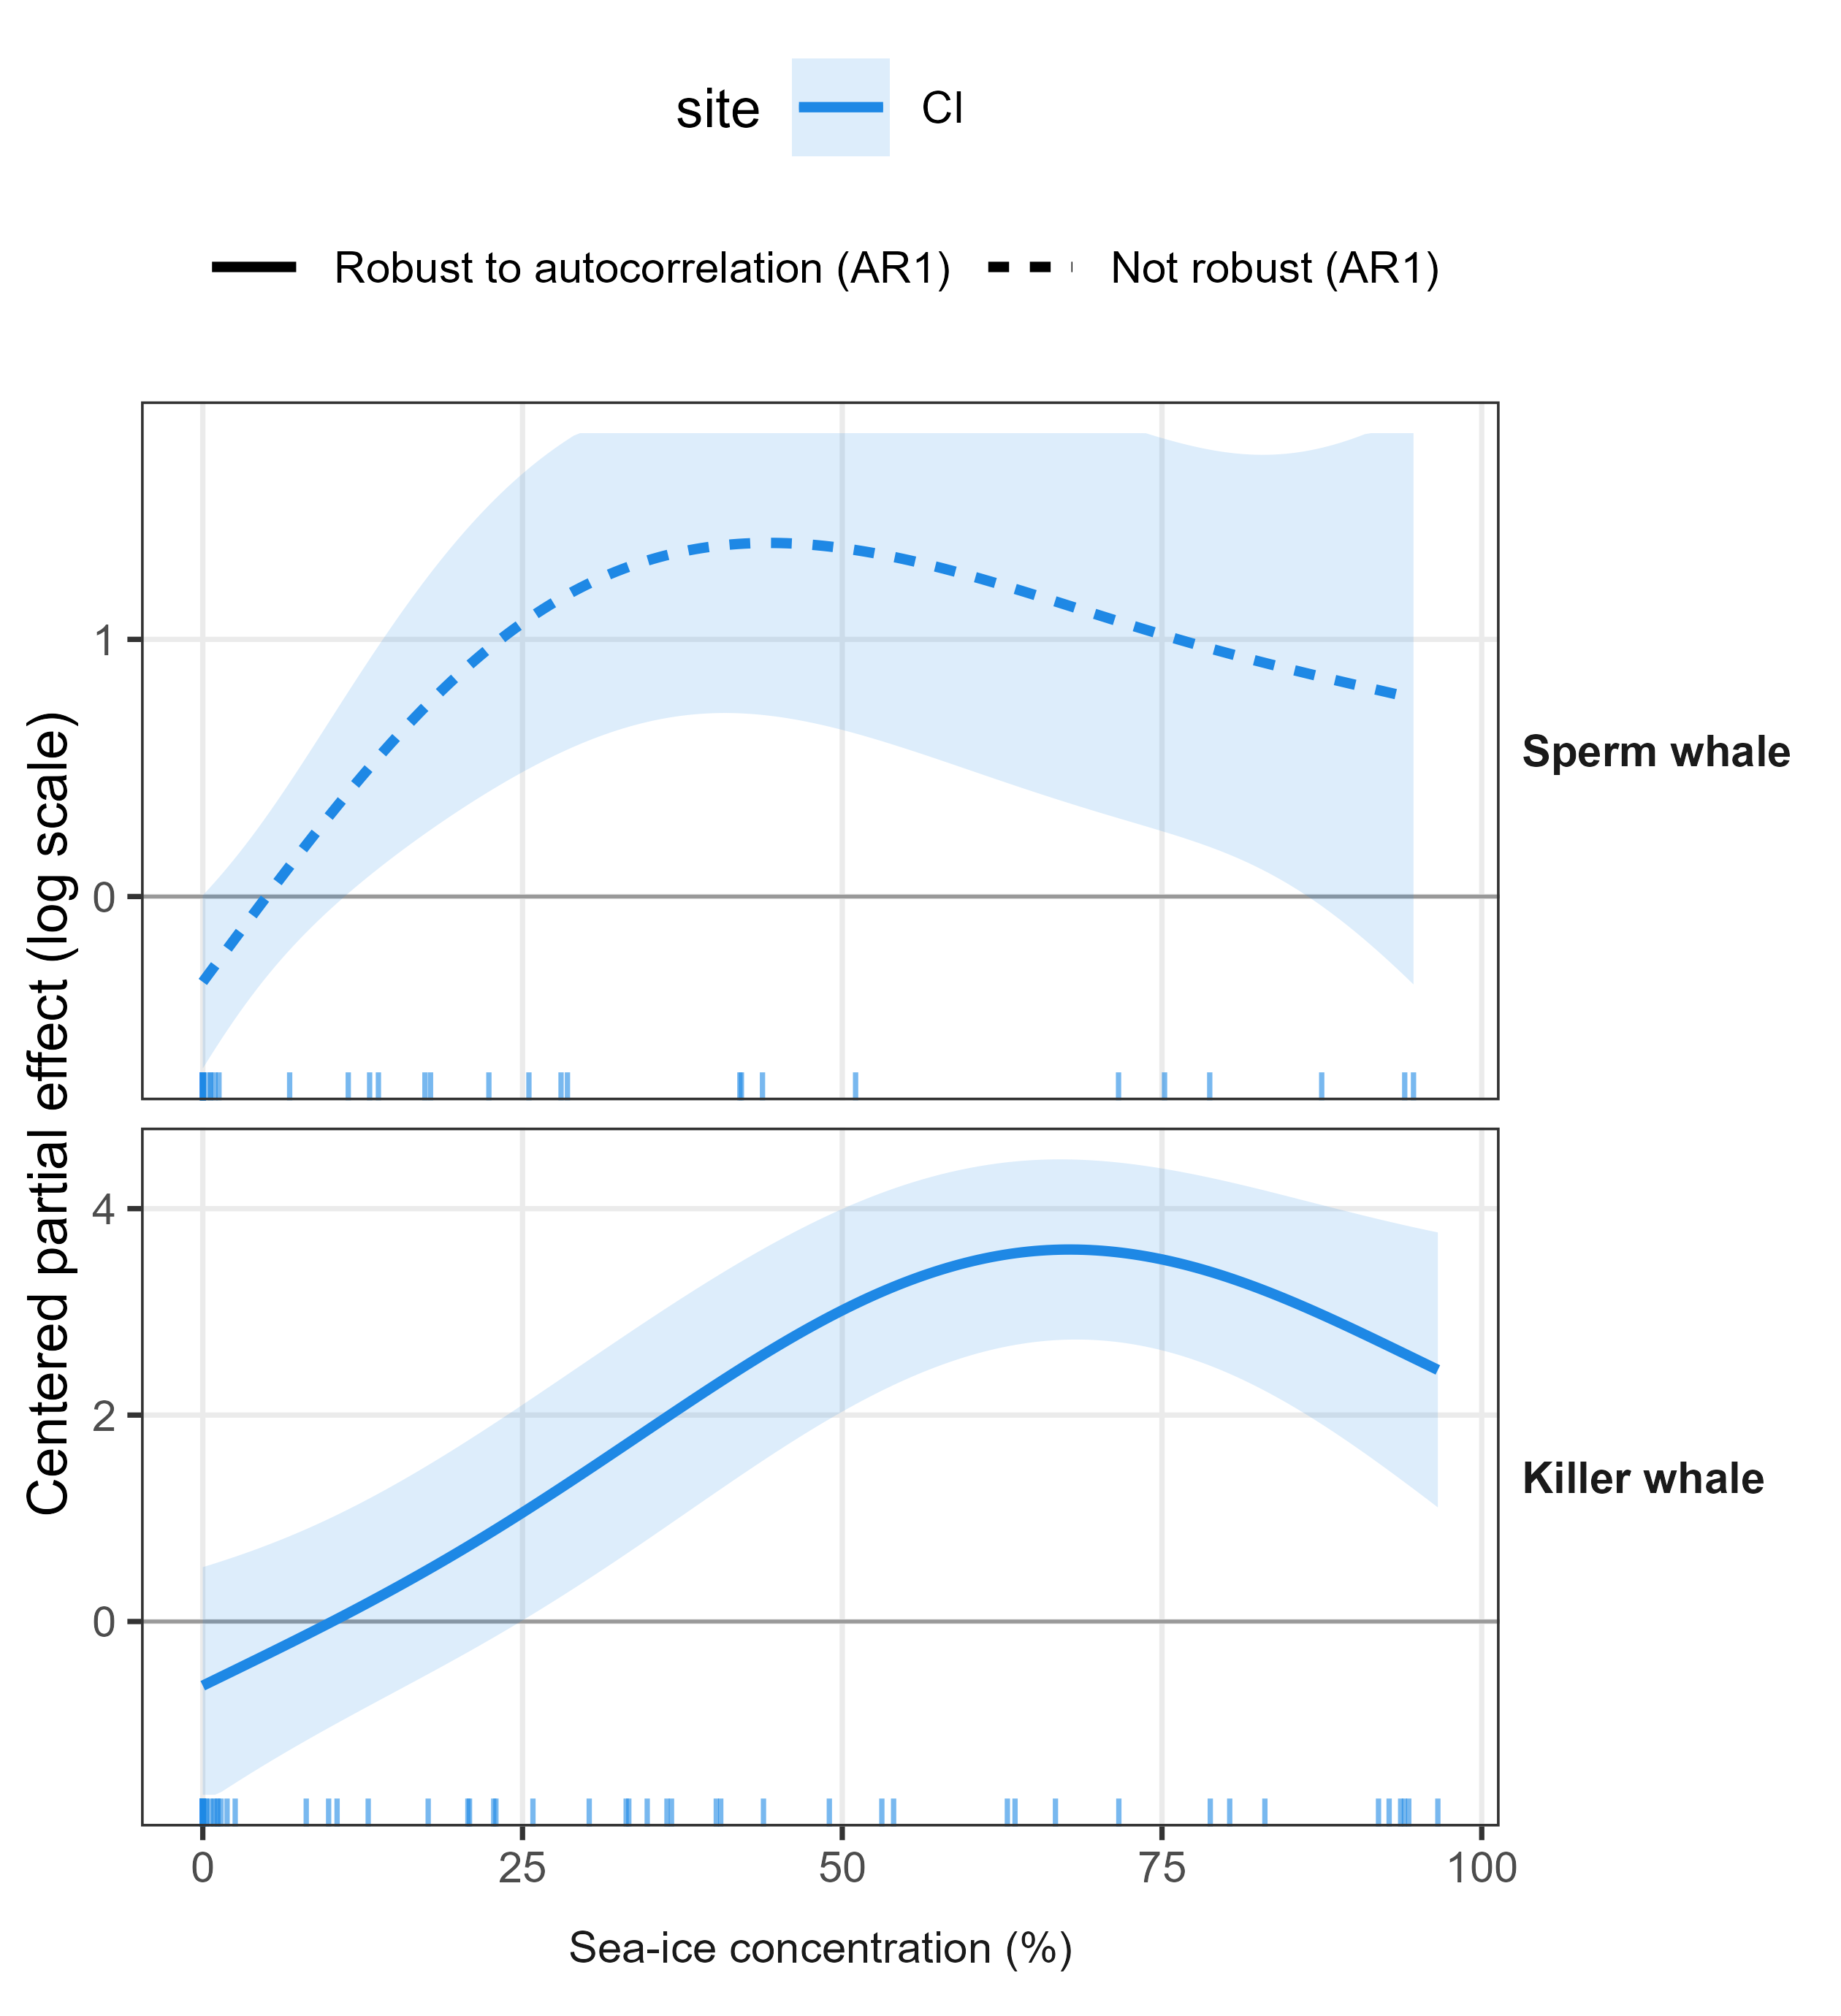
\includegraphics[width=1\linewidth,height=\textheight,keepaspectratio]{../outputs/08_results_gams/supplementary_sea_ice_response_curves.png}

}

\caption{\label{fig-icecurves}Centered partial effects (log scale) of
sea-ice concentration from the sea-ice GAMs, shown for models in which
the effect was significant (\(p\) ≤ 0.05), with 95\% confidence bands
(clipped at the panel limits) and the observed values of each bin (rug).
Solid lines: effects that remained significant when residual
autocorrelation was modeled with an AR(1) process; dashed lines: effects
that did not. Curves of southern bottlenose whales and BW37 end at the
highest sea-ice concentration at which the species was detected at that
site (2.9--5.1\%), because no detections occurred at higher
concentrations (34--36 bins) and the fitted decline beyond that point is
not estimable; these curves are re-centered over the range shown.}

\end{figure}%

\subsection*{S5. Habitat model diagnostics and sensitivity to residual
autocorrelation}\label{s5.-habitat-model-diagnostics-and-sensitivity-to-residual-autocorrelation}
\addcontentsline{toc}{subsection}{S5. Habitat model diagnostics and
sensitivity to residual autocorrelation}

AR(1) was supported (ΔAIC \textless{} −2) in 5 of 11 models: sperm
whales at EI and CI, long-finned pilot whales at KGI, killer whales at
CI, and southern bottlenose whales at EI. Across all models, 14 of the
24 testable terms remained significant (2 terms could not be tested
because a reduced model failed to converge). Under AR(1), lagged
chlorophyll-\emph{a} was not significant in any of the three models
where it could be tested (sperm whales at EI, killer whales at CI,
southern bottlenose whales at EI), nor were mixed layer depth (sperm
whales at EI and CI) or deep-layer EKE (sperm whales at CI). FSLE (sperm
whales at EI), FSLV orientation, mid-water EKE and surface-layer
temperature (sperm whales at CI), and surface-layer temperature (pilot
whales at KGI) remained significant. Three further terms were not
significant when refit by maximum likelihood even without AR(1) (pilot
whales at CI; mixed layer depth for BW37 at KGI). Effects that are not
robust are interpreted cautiously in the Discussion.
\conf{term-by-term sentences are typed; check against ar1\_sensitivity\_terms.csv after the final run}

\begin{table}[!h]
\centering
\caption{\label{tab:diagnostics}Diagnostics of the final habitat models. Tweedie p: estimated power parameter. Min k-index p: smallest p-value of the basis-dimension check across terms. Max concurvity: largest worst-case concurvity among terms. Lag-1 ACF and Ljung–Box p (lags 1--5 bins): residual autocorrelation; p ≤ 0.05 indicates remaining autocorrelation. ΔAIC with AR(1): change in AIC when an AR(1) process was added in glmmTMB (values < −2 indicate support for AR(1); -- = AR(1) model did not converge).}
\centering
\fontsize{8}{10}\selectfont
\begin{tabular}[t]{llrllllll}
\toprule
Species & Site & Bin (d) & Tweedie p & Min k-index p & Max concurvity & Lag-1 ACF & Ljung–Box p & ΔAIC with AR(1)\\
\midrule
Sperm whale & EI & 4 & 1.47 & 0.220 & 0.74 & 0.37 & 0.066 & -25.6\\
Sperm whale & CI & 4 & 1.57 & 0.122 & 0.88 & 0.04 & 0.170 & -23.1\\
Long-finned pilot whale & EI & 4 & 1.31 & 0.148 & 0.49 & -0.16 & 0.280 & --\\
Long-finned pilot whale & KGI & 4 & 1.32 & 0.948 & 0.00 & 0.44 & <0.001 & -5.7\\
Long-finned pilot whale & CI & 4 & 1.44 & 0.400 & 0.25 & 0.11 & 0.160 & 2.9\\
Killer whale & CI & 2 & 1.35 & 0.660 & 0.00 & 0.12 & 0.340 & -19.1\\
Southern bottlenose whale & EI & 4 & 1.50 & 0.295 & 0.71 & -0.21 & 0.350 & -3.6\\
Southern bottlenose whale & KGI & 4 & 1.18 & 0.050 & 0.00 & 0.27 & 0.140 & --\\
Southern bottlenose whale & CI & 4 & 1.39 & 0.265 & 0.71 & 0.35 & 0.034 & 3.2\\
BW37 beaked whale & EI & 4 & 1.10 & 0.540 & 0.26 & 0.01 & 0.470 & 2.0\\
BW37 beaked whale & KGI & 4 & 1.17 & 0.530 & 0.06 & -0.10 & 0.580 & 2.2\\
\bottomrule
\end{tabular}
\end{table}

\subsection*{S6. Species--site combinations not
modeled}\label{s6.-speciessite-combinations-not-modeled}
\addcontentsline{toc}{subsection}{S6. Species--site combinations not
modeled}

\begin{table}[!h]
\centering
\caption{\label{tab:rare}Conditions on detection days for species--site combinations with too few detections to model (<10 bins with detections). EKE percentile: position of the median EKE on detection days among all recording days at that site. Sperm whales were never detected at KGI.}
\centering
\fontsize{8}{10}\selectfont
\begin{tabular}[t]{>{\raggedright\arraybackslash}p{2.2cm}>{\raggedleft\arraybackslash}p{1.5cm}>{\raggedright\arraybackslash}p{2.3cm}>{\raggedright\arraybackslash}p{2.8cm}>{\raggedright\arraybackslash}p{2.8cm}>{\raggedright\arraybackslash}p{3cm}}
\toprule
Species, site & Detection days & Months & Sea-ice cover on detection days & EKE (percentile among recording days) & Other conditions\\
\midrule
Killer whale, EI & 3 & Mar, May, Jun 2014 & 0–0.4\% & 73rd–74th (mid-water, deep) & typical\\
Killer whale, KGI & 3 & May, Jul, Oct 2015 & 1\% (26 May), 10\% (2 Jul), 70\% (5 Oct) & 94th–97th (mid-water, deep) & surface layer warmer than usual (81st percentile)\\
BW37, CI & 11 & Mar–Apr, Nov 2016 & 0\% (all days) & 83rd (deep) & typical\\
\bottomrule
\end{tabular}
\end{table}

\subsection*{S7. Supplementary occurrence
figures}\label{s7.-supplementary-occurrence-figures}
\addcontentsline{toc}{subsection}{S7. Supplementary occurrence figures}

\begin{figure}[htbp]

\centering{

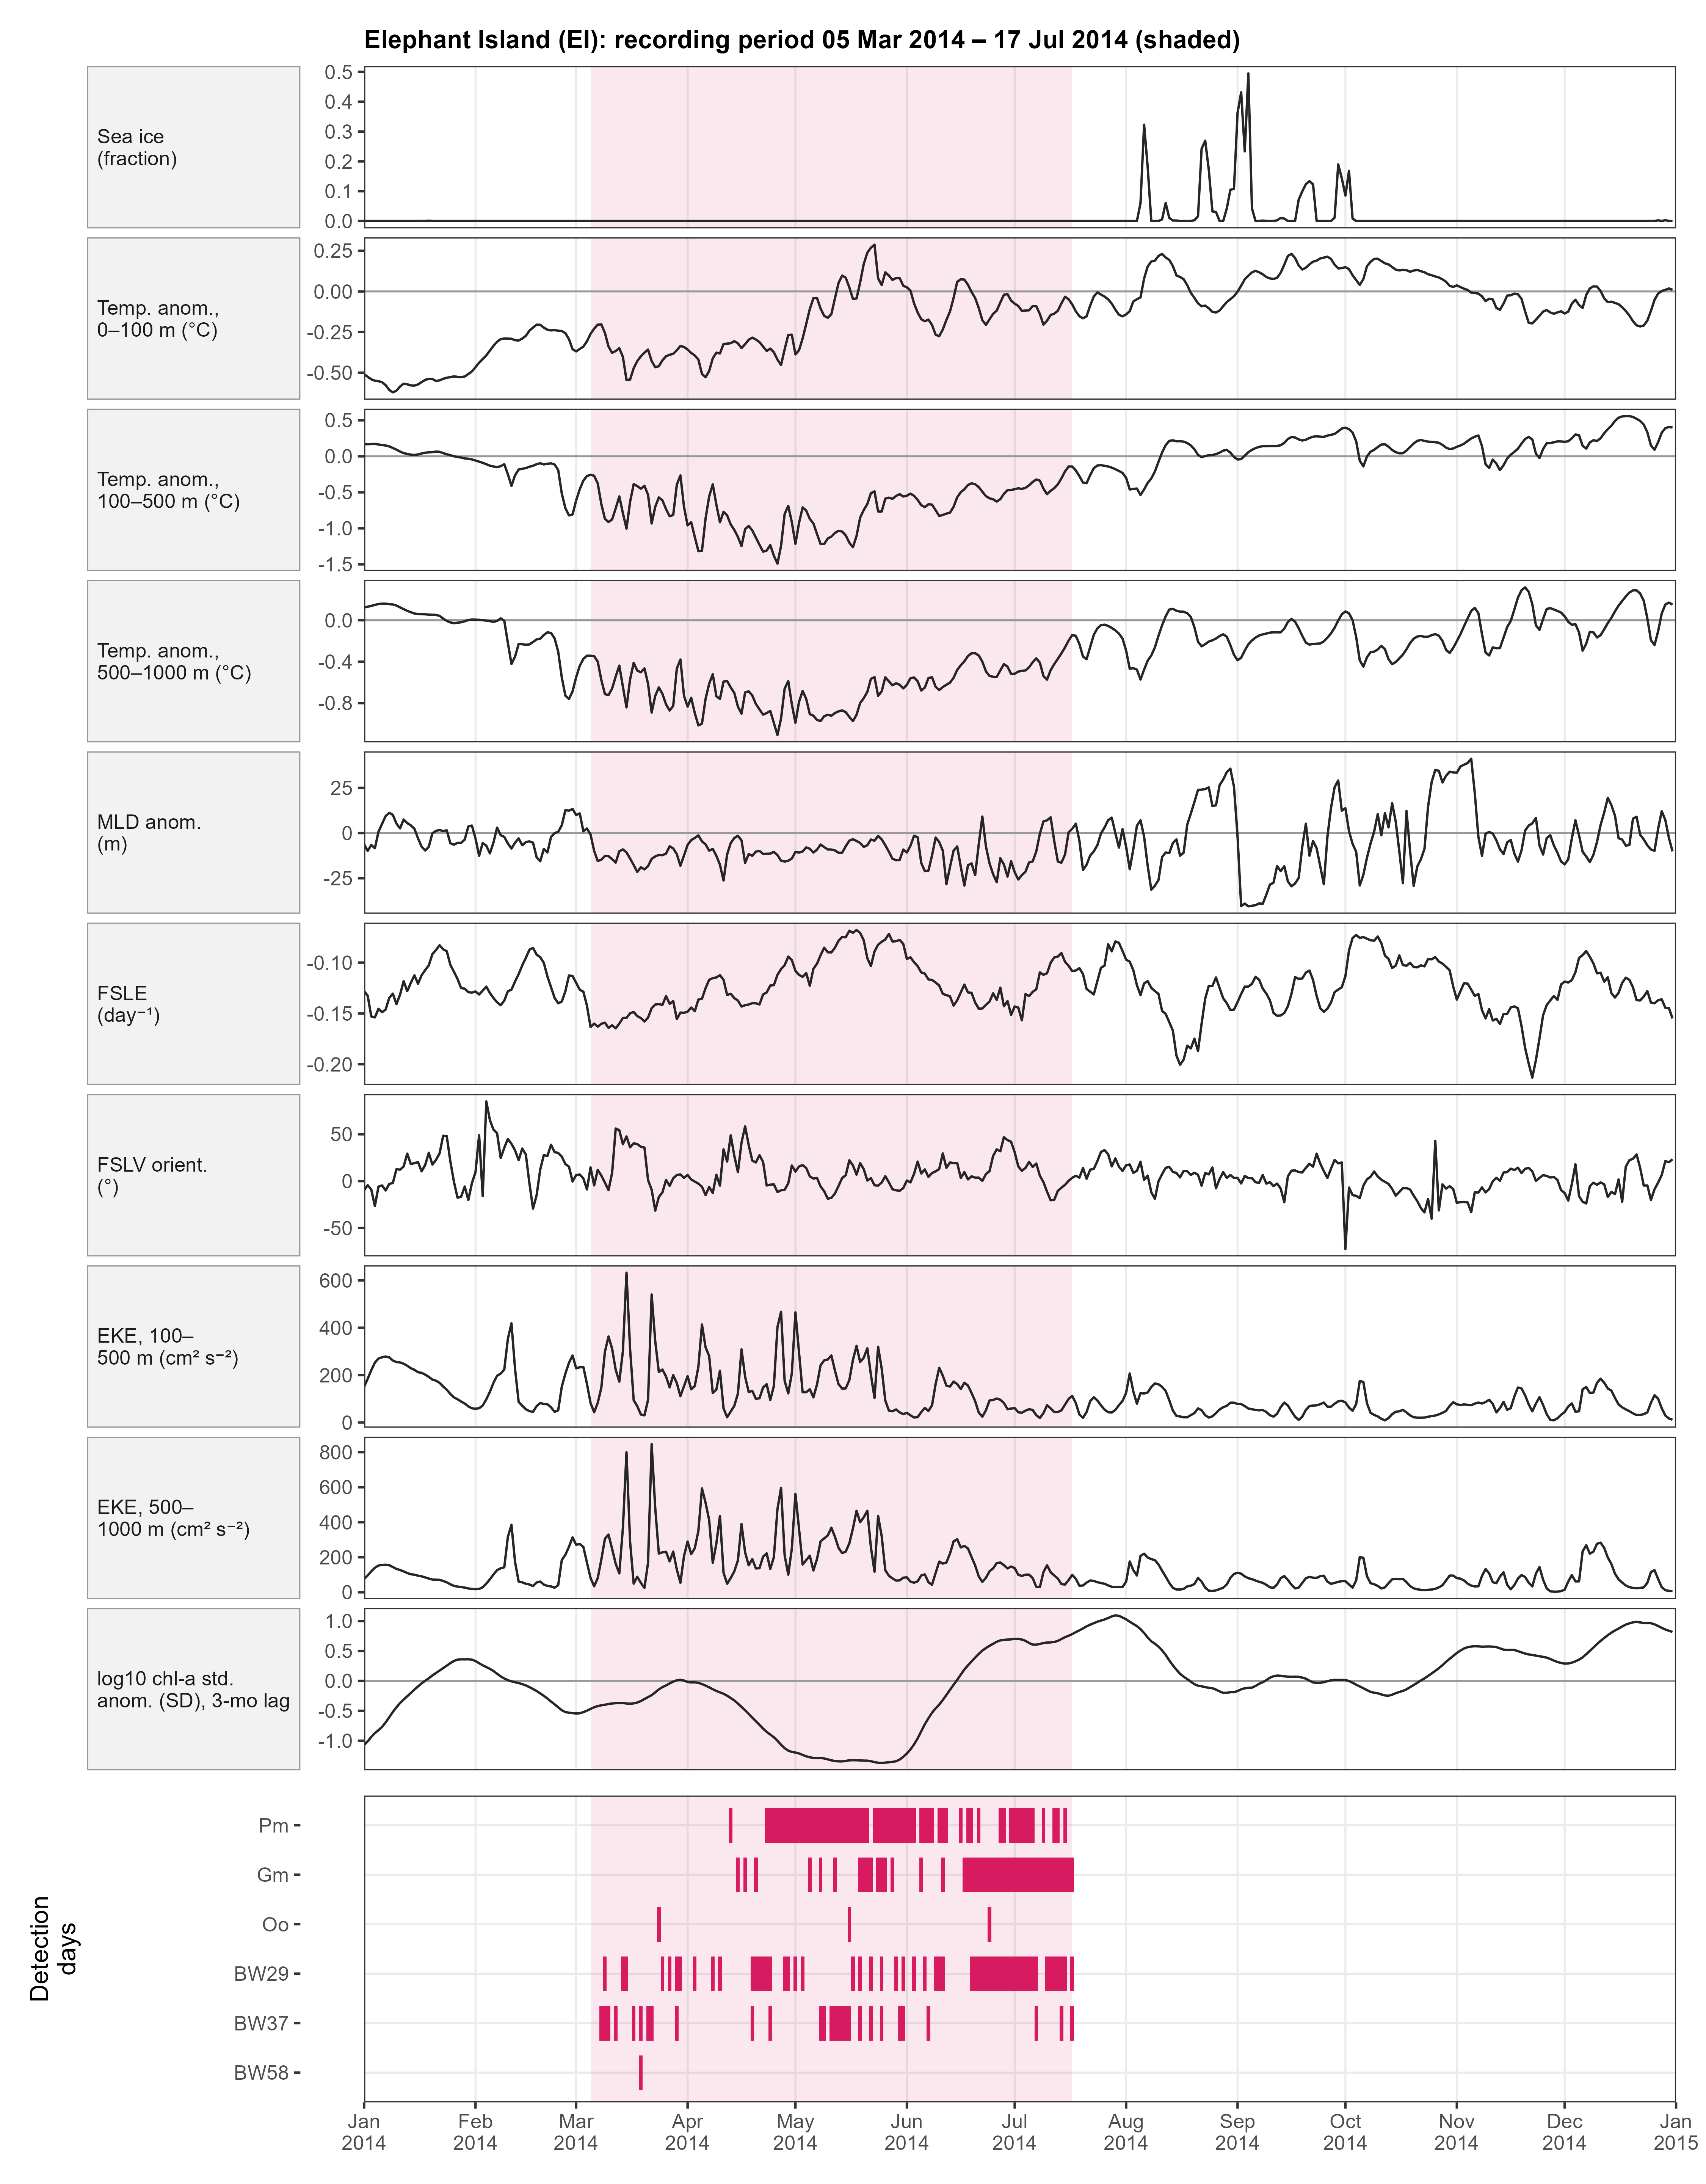
\includegraphics[width=1\linewidth,height=\textheight,keepaspectratio]{../outputs/07_results_occurrence/figS_env_presence_EI.png}

}

\caption{\label{fig-envEI}Acoustic presence and the final model
predictors (anomalies by layer) at EI. \ins{Legend to be drafted}}

\end{figure}%

\begin{figure}[htbp]

\centering{

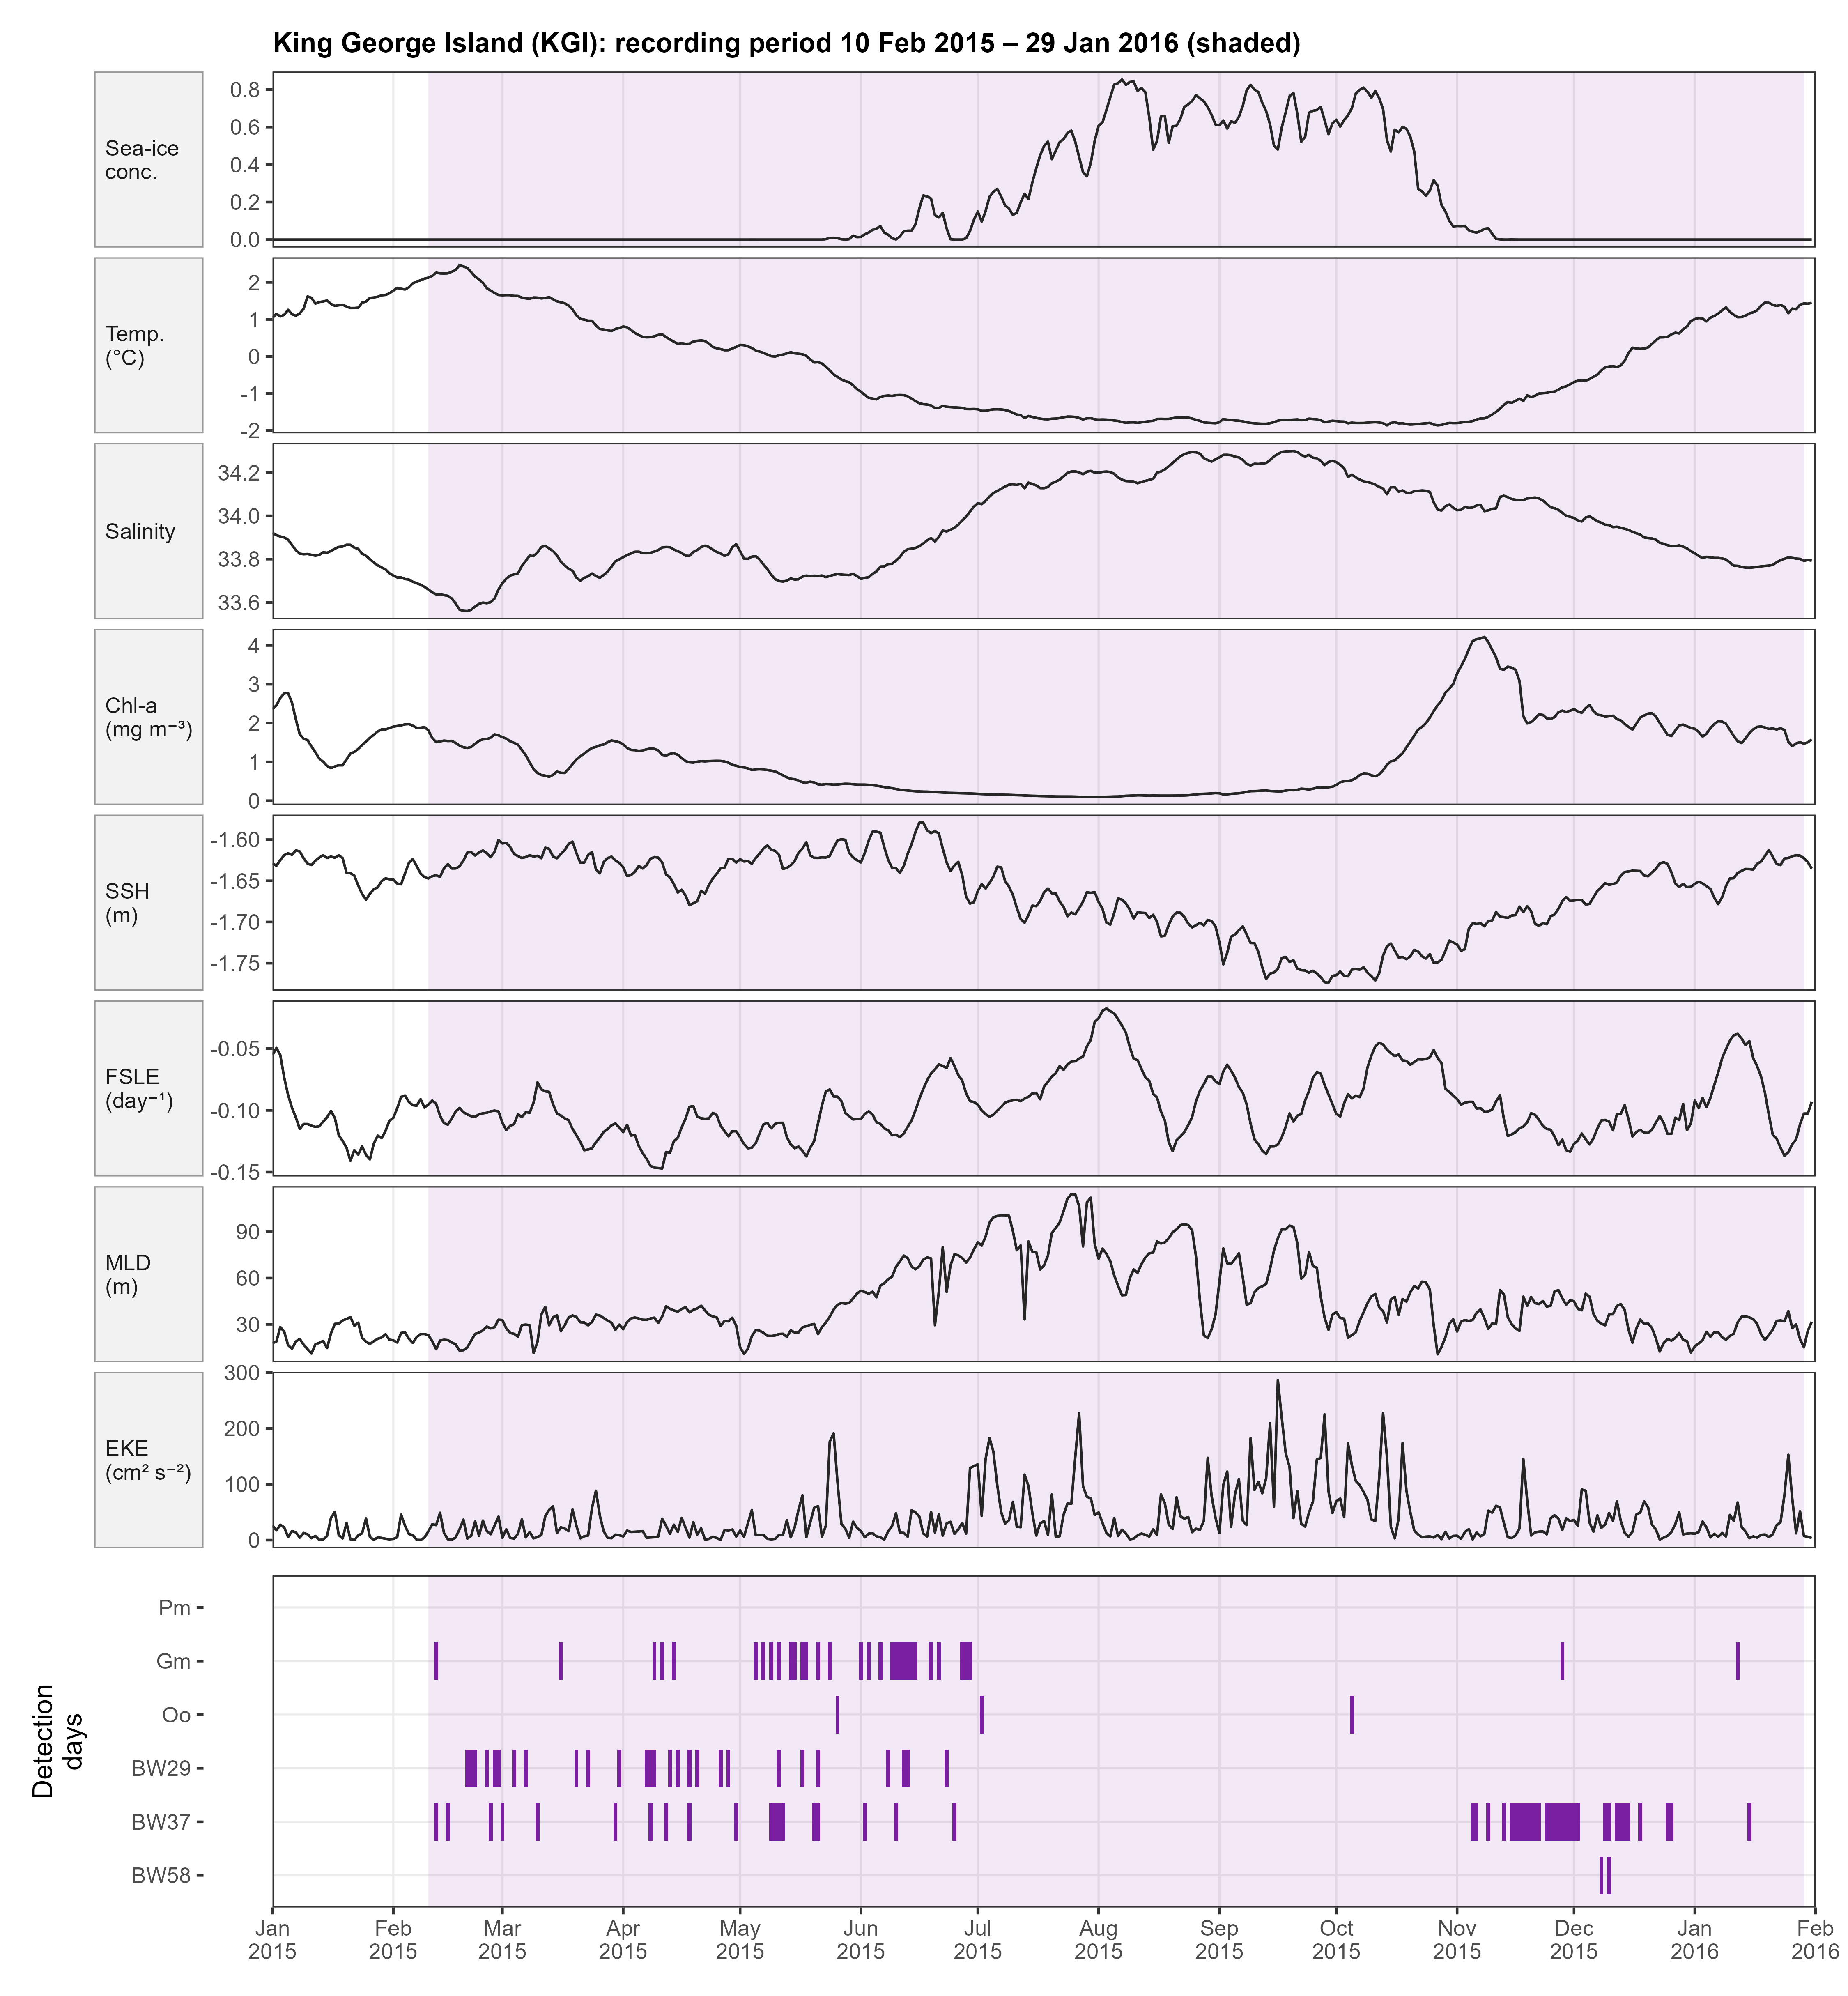
\includegraphics[width=1\linewidth,height=\textheight,keepaspectratio]{../outputs/07_results_occurrence/figS_env_presence_KGI.png}

}

\caption{\label{fig-envKGI}As Figure~\ref{fig-envEI}, for KGI.}

\end{figure}%

\begin{figure}[htbp]

\centering{

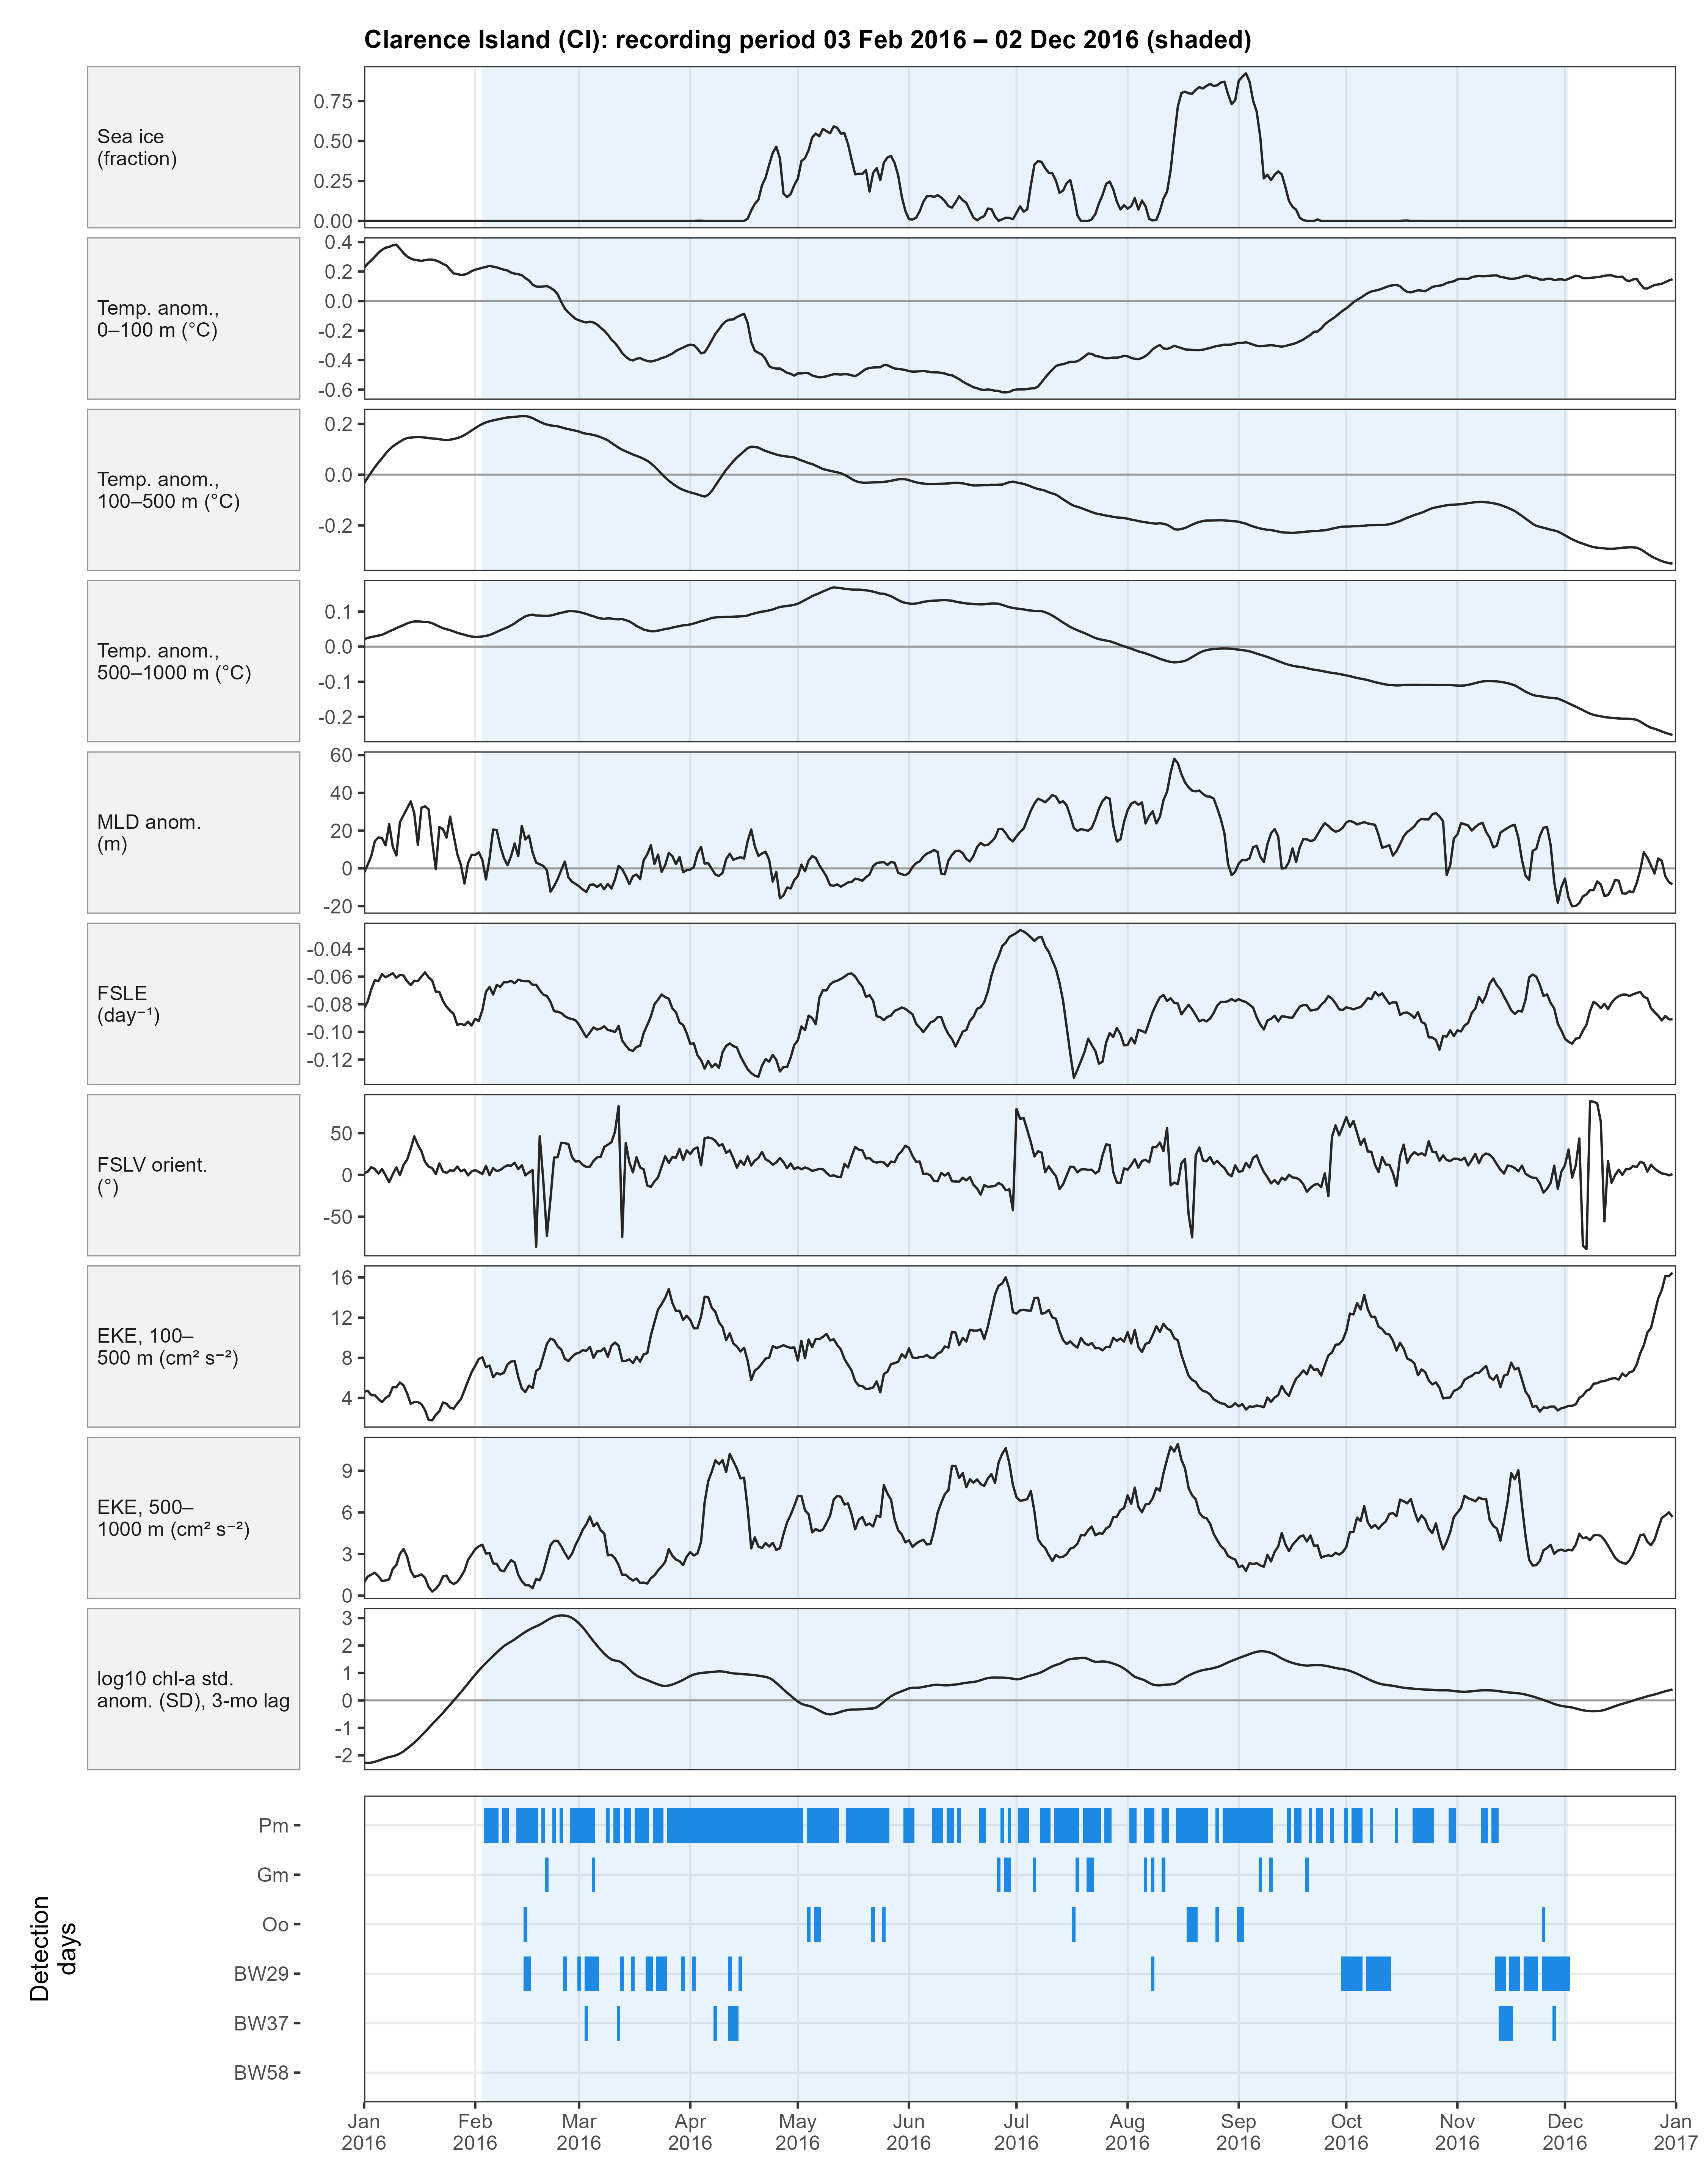
\includegraphics[width=1\linewidth,height=\textheight,keepaspectratio]{../outputs/07_results_occurrence/figS_env_presence_CI.png}

}

\caption{\label{fig-envCI}As Figure~\ref{fig-envEI}, for CI.}

\end{figure}%

\begin{figure}[htbp]

\centering{

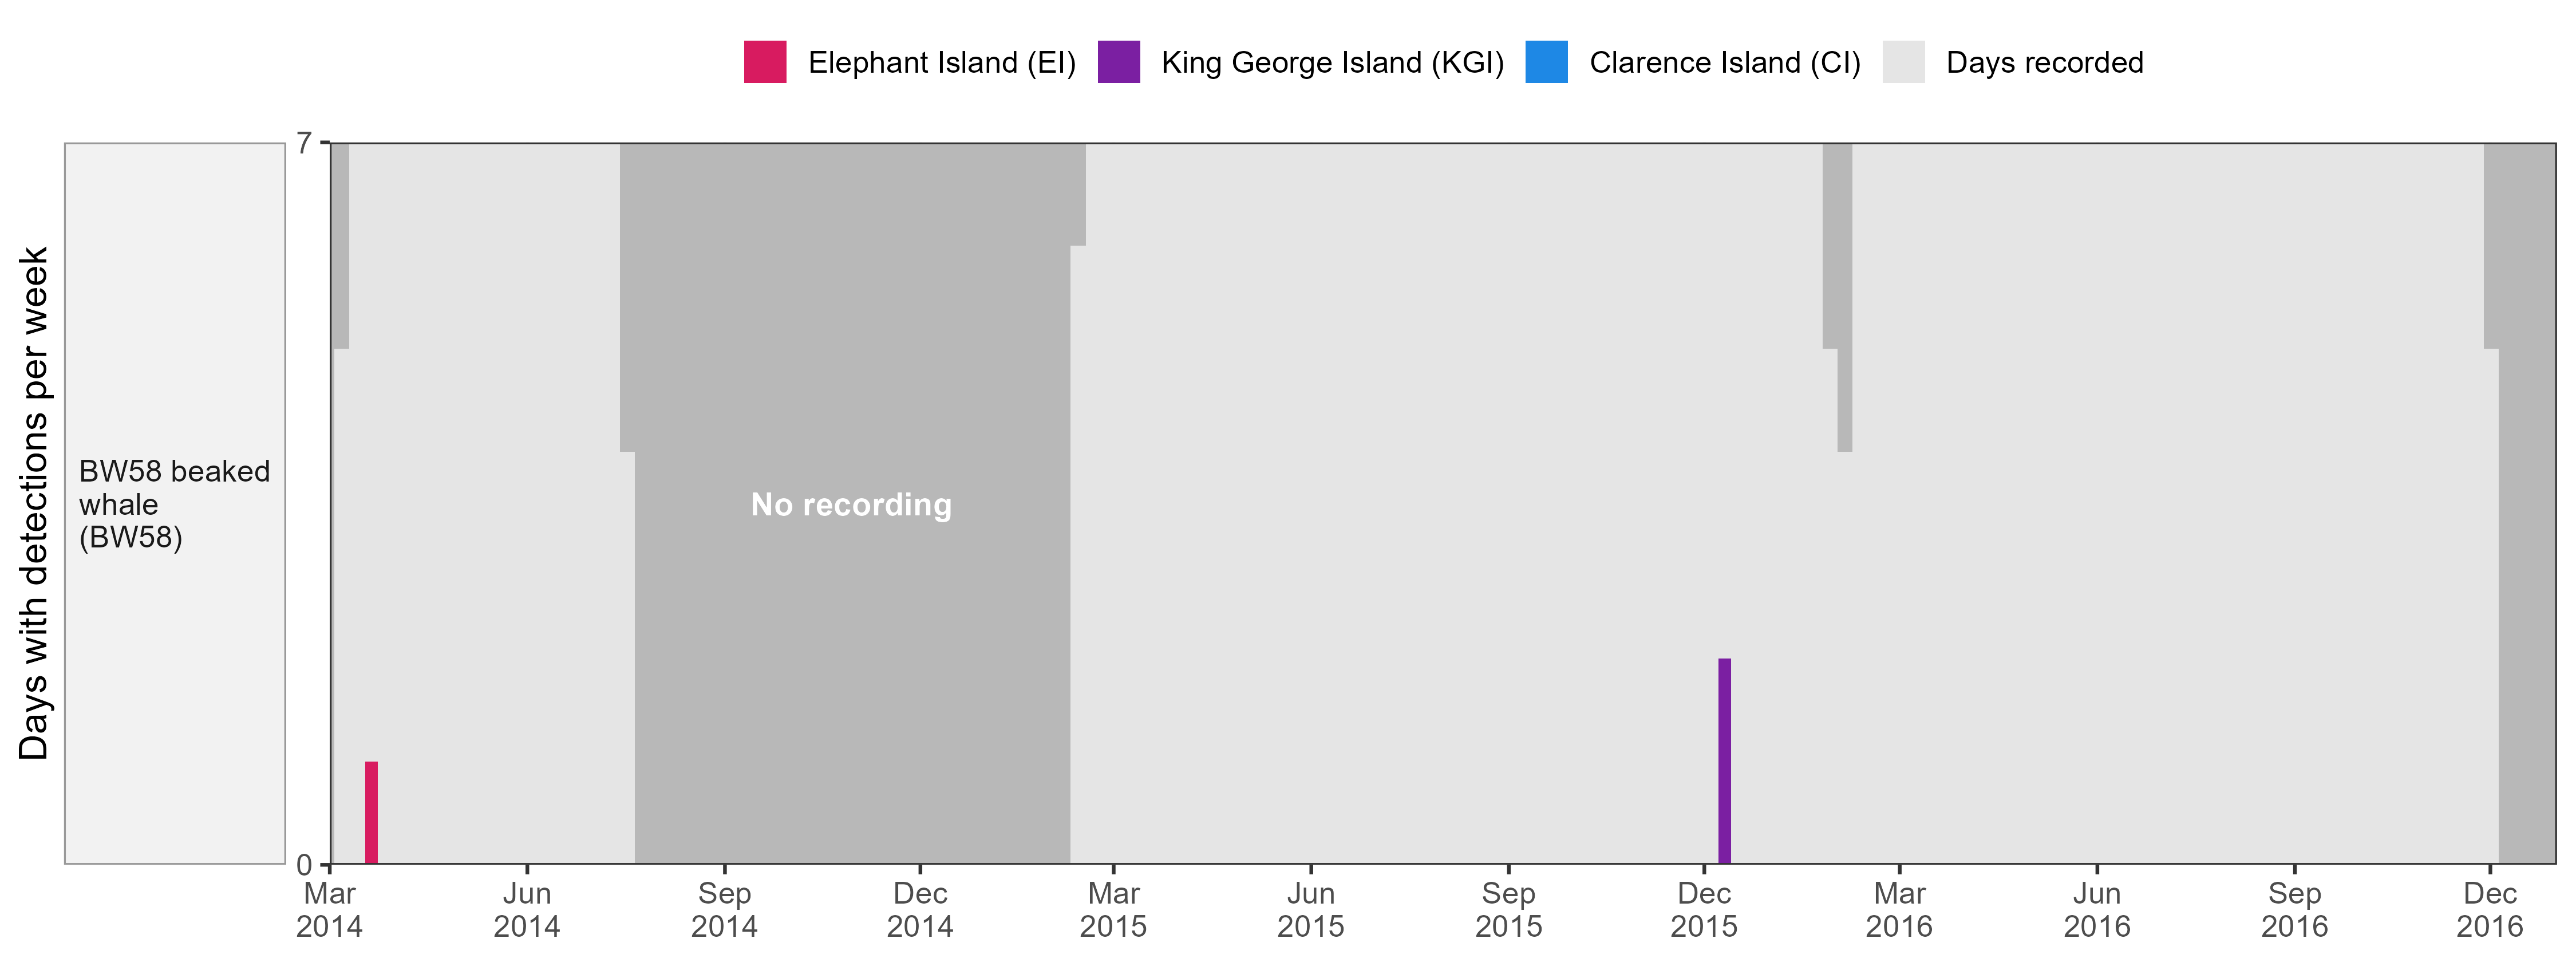
\includegraphics[width=1\linewidth,height=\textheight,keepaspectratio]{../outputs/07_results_occurrence/figS_weekly_presence_BW58.png}

}

\caption{\label{fig-bw58}Weekly acoustic presence of the BW58 beaked
whale signal type. \ins{Legend to be drafted}}

\end{figure}%




\end{document}
